\documentclass[12pt,a4paper]{article}

\usepackage[utf8]{inputenc}
\usepackage[T1]{fontenc}
\usepackage{geometry}
\usepackage{graphicx}
\usepackage{booktabs}
\usepackage{hyperref}
\usepackage{listings}
\usepackage{xcolor}
\usepackage{amsmath}
\usepackage{amssymb}
\usepackage{float}
\usepackage{caption}
\usepackage{subcaption}
\usepackage{parskip}
\usepackage{tikz}
\usetikzlibrary{decorations.pathreplacing, positioning, arrows.meta, shapes.geometric}
\usepackage[most]{tcolorbox}

\geometry{margin=2.5cm}

\hypersetup{
    colorlinks=true,
    linkcolor=blue,
    urlcolor=blue,
    citecolor=blue,
    pdfstartpage=1,
    pdfstartview=FitH
}

\lstset{
    basicstyle=\ttfamily\small,
    breaklines=true,
    frame=single,
    backgroundcolor=\color{gray!10}
}

\title{\textbf{EGFR Variant Detection Panel Validation}}
\author{}
\date{\today}

\begin{document}

\maketitle

\begin{abstract}
This report presents a bioinformatic validation of a targeted amplicon sequencing
panel designed to detect clinically actionable mutations in the \textit{EGFR} gene
(epidermal growth factor receptor) relevant to non-small-cell lung cancer (NSCLC).
The panel covers four amplicons spanning the key mutation hotspots in exons~18--21,
including the exon~19 in-frame deletions (e.g.\ E746\_A750del) and the exon~21 L858R
substitution that confer sensitivity to tyrosine kinase inhibitors (TKIs) such as
gefitinib, erlotinib, and osimertinib.

Using a single paired-end Illumina sequencing run (pre-aligned BAM, hg19), the
analysis addresses five validation questions: (1) read constitution and adaptor
content, (2) target gene identification by BLAST-based primer alignment,
(3) overall mapping rate and read quality, (4) per-amplicon coverage depth and
uniformity, and (5) somatic variant calling with orthogonal callers (Mutect2,
VarDictJava).
The analysis was implemented as a reproducible Snakemake pipeline running inside
a Docker container, with all results compiled into this report.

Key findings: all four amplicons amplify on-target EGFR exon sequences;
mapping rates exceed 99\%; per-amplicon depth is uniformly high
($>$1{,}000$\times$) for three amplicons, with Amplicon~2 showing
substantially lower coverage ($\sim$9{,}000 vs.\ $\sim$200{,}000 read pairs)
attributable to primer inefficiency.
Furthermore, 89\% of Amplicon~2 read pairs are unmapped: BLAST analysis of a
random subsample of 200 R1 reads (saved as \texttt{amp2\_unmapped\_sample.fa})
identifies 87\% as originating from bacteriophage $\phi$X174
(\textit{Sinsheimervirus phiX174}), the standard Illumina sequencing
spike-in, indicating that the Amplicon~2 forward primer cross-reacts with
the phage genome during PCR.
Both findings suggest that the Amplicon~2 primer pair warrants redesign.
One confirmed somatic EGFR driver mutation was identified: the exon~19
in-frame deletion E746\_A750del (VAF~48\%, VarDictJava, COSM6223),
annotated by SnpEff as \texttt{p.Glu746\_Ala750del} using the hg19 database.
T790M and L858R are absent, confirmed by high-depth coverage ($>$200{,}000$\times$)
at both hotspot positions with no PASS calls.
A germline SNP at chr7:55{,}249{,}063 (rs1050171, EGFR Gln787Gln,
synonymous) was flagged by both callers in tumour-only mode, illustrating the
need for population germline filtering or a matched normal in clinical workflows.
Two additional Mutect2 PASS calls at amplicon boundaries are primer-end artefacts
caused by the absence of primer trimming (\texttt{ivar trim}) in the original
BAM processing; these must be filtered before clinical reporting.
\end{abstract}

\clearpage
\tableofcontents
\clearpage

% ============================================================
\section{Biological Background: EGFR and Lung Cancer}
\label{sec:egfr-background}
% ============================================================

\paragraph{Clinical use of EGFR mutation testing in lung cancer.}
Non-small-cell lung cancer (NSCLC) accounts for approximately 85\% of all
lung cancer cases and carries a poor prognosis when diagnosed at advanced
stage.
In roughly 10--15\% of Western and 30--40\% of East Asian NSCLC patients,
the tumour is driven by an activating mutation in the \textit{EGFR} gene.
These patients are identified at diagnosis by targeted sequencing of the
EGFR kinase domain (exons 18--21), which is now a mandatory step before
initiating systemic therapy.
A positive result directly determines the treatment choice: EGFR-mutant
patients receive an oral EGFR tyrosine kinase inhibitor (TKI)\footnote{%
  A tyrosine kinase inhibitor is a small molecule drug that blocks the
  enzymatic activity of a kinase --- a protein that switches other proteins
  on or off by attaching phosphate groups to them.
  EGFR is a receptor tyrosine kinase: when mutated, it is permanently
  switched on, driving uncontrolled cell growth.
  A TKI fits into the active site of the kinase and blocks this signal,
  effectively turning the driver mutation off.} rather than conventional
chemotherapy, with substantially better response rates and
tolerability~\cite{lynch2004}.

\paragraph{Tyrosine kinase inhibitor generations.}
A \textbf{sensitising mutation} is one that makes the tumour cells vulnerable to
a TKI: the mutation keeps EGFR permanently active, and the drug binds to
exactly that active conformation to switch it off.
Without the mutation, the drug has no specific target and normal EGFR function
would be disrupted.
E746\_A750del, L858R, and G719X are classic sensitising mutations; patients
whose tumours carry them respond strongly to TKIs, whereas those without an
EGFR sensitising mutation do not benefit.

Three generations of EGFR-targeted TKIs have been developed, each
designed to overcome limitations of the previous one:
\begin{itemize}
  \item \textbf{First generation} (gefitinib, erlotinib): the original
        EGFR inhibitors, in clinical use since 2003--2004.
        Effective against the common sensitising mutations but overcome by
        resistance in most patients within 12--18 months, primarily through
        acquisition of T790M.
  \item \textbf{Second generation} (afatinib, dacomitinib): approved
        from 2013 onwards; more potent and active against a broader range
        of mutations including G719X, but still overcome by T790M.
  \item \textbf{Third generation} (osimertinib): approved in 2015
        initially for T790M-positive patients who had progressed on a
        prior TKI, and in 2018 as first-line therapy for all sensitising
        mutations due to superior progression-free survival and CNS
        penetration.
\end{itemize}
The clinical consequence is that the sequencing result not only confirms
whether the patient is EGFR-mutant, but also which generation of TKI is
appropriate: a treatment-na\"{i}ve patient with L858R receives osimertinib
(or a 1st/2nd-gen agent); a patient who has progressed on a 1st-gen TKI
and newly acquired T790M is switched to osimertinib.
Figure~\ref{fig:tki-decision} summarises the decision logic.

\begin{figure}[H]
  \centering
  \resizebox{\linewidth}{!}{% TKI treatment decision tree based on EGFR panel result.
% Included via % TKI treatment decision tree based on EGFR panel result.
% Included via % TKI treatment decision tree based on EGFR panel result.
% Included via \input{figures/tki_decision_tree} inside a figure environment.

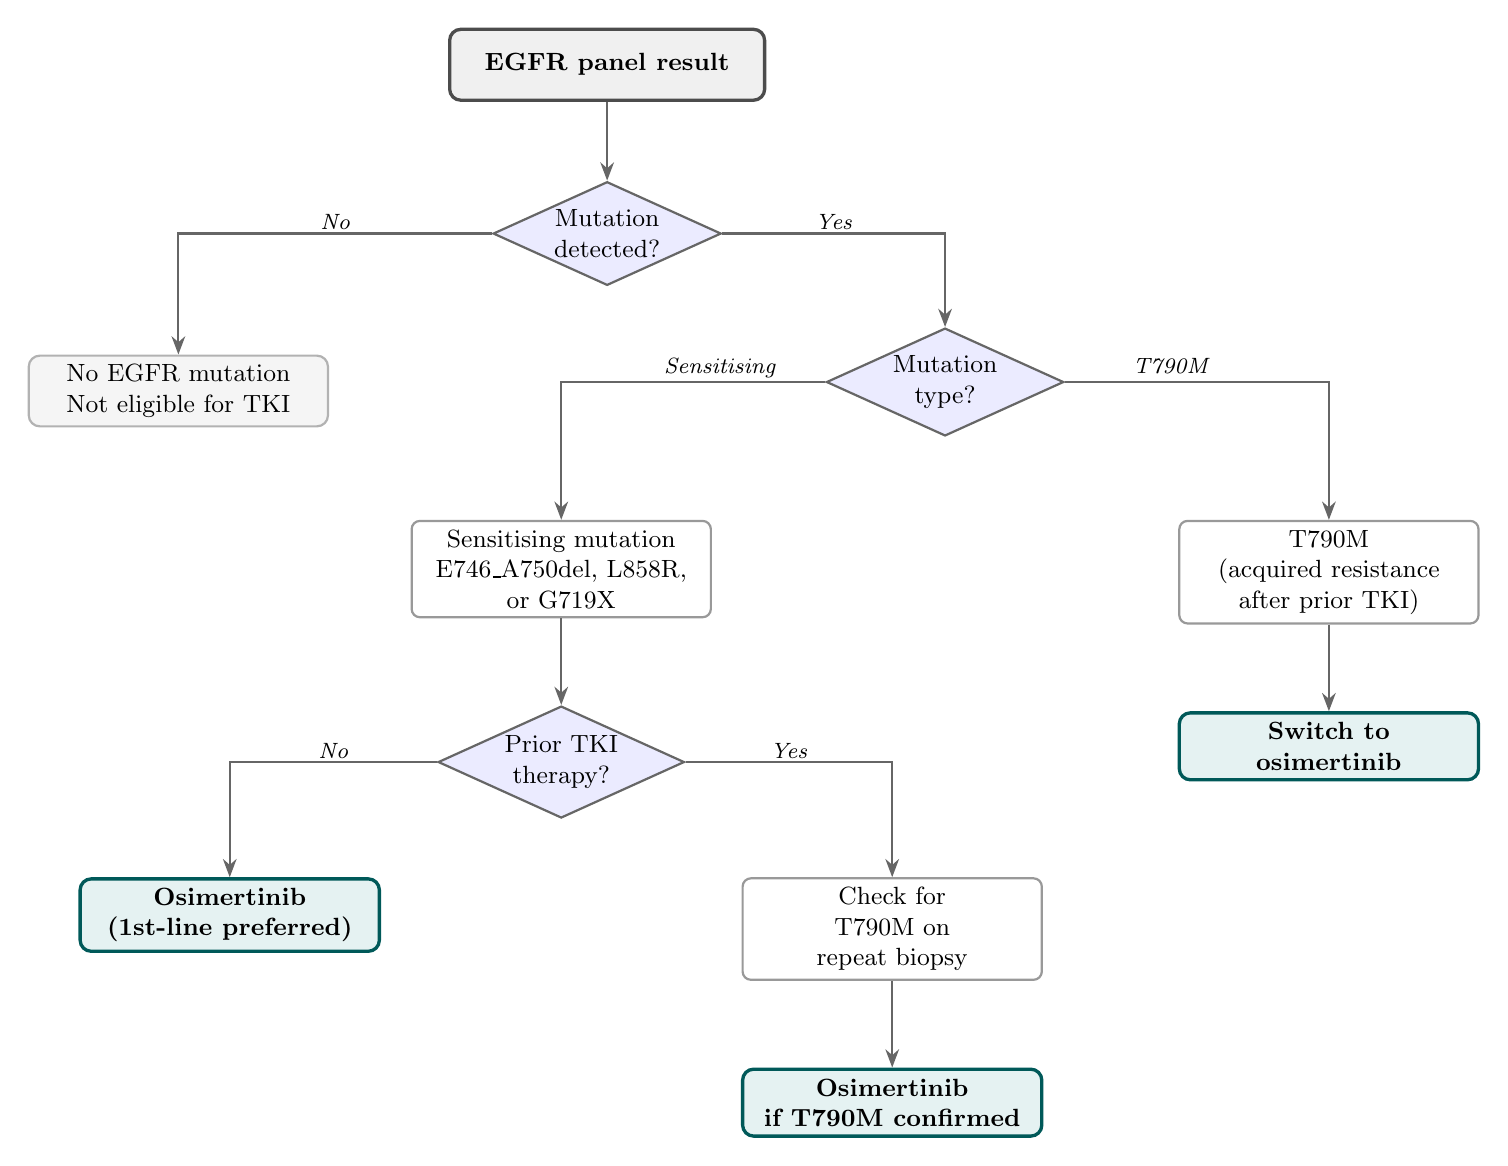
\begin{tikzpicture}[
  node distance = 0.6cm and 1.8cm,
  % Styles
  start/.style   = {rectangle, draw=black!70, very thick, fill=gray!12,
                    rounded corners=4pt, align=center, font=\small\bfseries,
                    minimum width=4cm, minimum height=0.9cm},
  decision/.style = {diamond, draw=black!60, thick, fill=blue!8,
                    align=center, font=\small, inner sep=1pt,
                    aspect=2.2},
  result/.style   = {rectangle, draw=black!40, thick, fill=white,
                    rounded corners=3pt, align=center, font=\small,
                    minimum width=3.8cm, minimum height=0.85cm},
  treat/.style    = {rectangle, draw=teal!70!black, very thick,
                    fill=teal!10, rounded corners=4pt, align=center,
                    font=\small\bfseries,
                    minimum width=3.8cm, minimum height=0.85cm},
  notreat/.style  = {rectangle, draw=gray!60, thick, fill=gray!8,
                    rounded corners=4pt, align=center, font=\small,
                    minimum width=3.8cm, minimum height=0.85cm},
  arrow/.style    = {->, >=Stealth, thick, draw=black!60},
  lbl/.style      = {font=\footnotesize\itshape, fill=white,
                    inner sep=1pt},
]

%% ── Nodes ──────────────────────────────────────────────────────────────────

% Root
\node[start] (panel) {EGFR panel result};

% Decision 1: mutation detected?
\node[decision, below=1.0cm of panel] (mut_q)
      {Mutation\\detected?};

% Left branch: no mutation
\node[notreat, below left=1.2cm and 2.8cm of mut_q] (no_mut)
      {No EGFR mutation\\Not eligible for TKI};

% Right branch: mutation detected → which type?
\node[decision, below right=1.2cm and 2.8cm of mut_q] (type_q)
      {Mutation\\type?};

% Sensitising branch (left of type_q)
\node[result, below left=1.4cm and 2.2cm of type_q] (sensitising)
      {Sensitising mutation\\E746\_A750del, L858R,\\or G719X};

% T790M branch (right of type_q)
\node[result, below right=1.4cm and 2.2cm of type_q] (t790m_node)
      {T790M\\(acquired resistance\\after prior TKI)};

% Treatment: sensitising → further question: naïve vs resistant?
\node[decision, below=1.1cm of sensitising] (naive_q)
      {Prior TKI\\therapy?};

\node[treat, below left=1.1cm and 1.5cm of naive_q] (osi_first)
      {Osimertinib\\(1st-line preferred)};

\node[result, below right=1.1cm and 1.5cm of naive_q] (check_t790m)
      {Check for\\T790M on\\repeat biopsy};

% Treatment: T790M → osimertinib
\node[treat, below=1.1cm of t790m_node] (osi_switch)
      {Switch to\\osimertinib};

% Treatment after repeat biopsy
\node[treat,  below=1.1cm of check_t790m] (osi_if)
      {Osimertinib\\if T790M confirmed};

%% ── Arrows ─────────────────────────────────────────────────────────────────

\draw[arrow] (panel)    -- (mut_q);

\draw[arrow] (mut_q)    -| node[lbl, above, pos=0.25] {No}  (no_mut);
\draw[arrow] (mut_q)    -| node[lbl, above, pos=0.25] {Yes} (type_q);

\draw[arrow] (type_q)   -| node[lbl, above, pos=0.2] {Sensitising} (sensitising);
\draw[arrow] (type_q)   -| node[lbl, above, pos=0.2] {T790M}       (t790m_node);

\draw[arrow] (sensitising) -- (naive_q);

\draw[arrow] (naive_q)  -| node[lbl, above, pos=0.25] {No}  (osi_first);
\draw[arrow] (naive_q)  -| node[lbl, above, pos=0.25] {Yes} (check_t790m);

\draw[arrow] (t790m_node) -- (osi_switch);
\draw[arrow] (check_t790m)  -- (osi_if);

\end{tikzpicture}
 inside a figure environment.

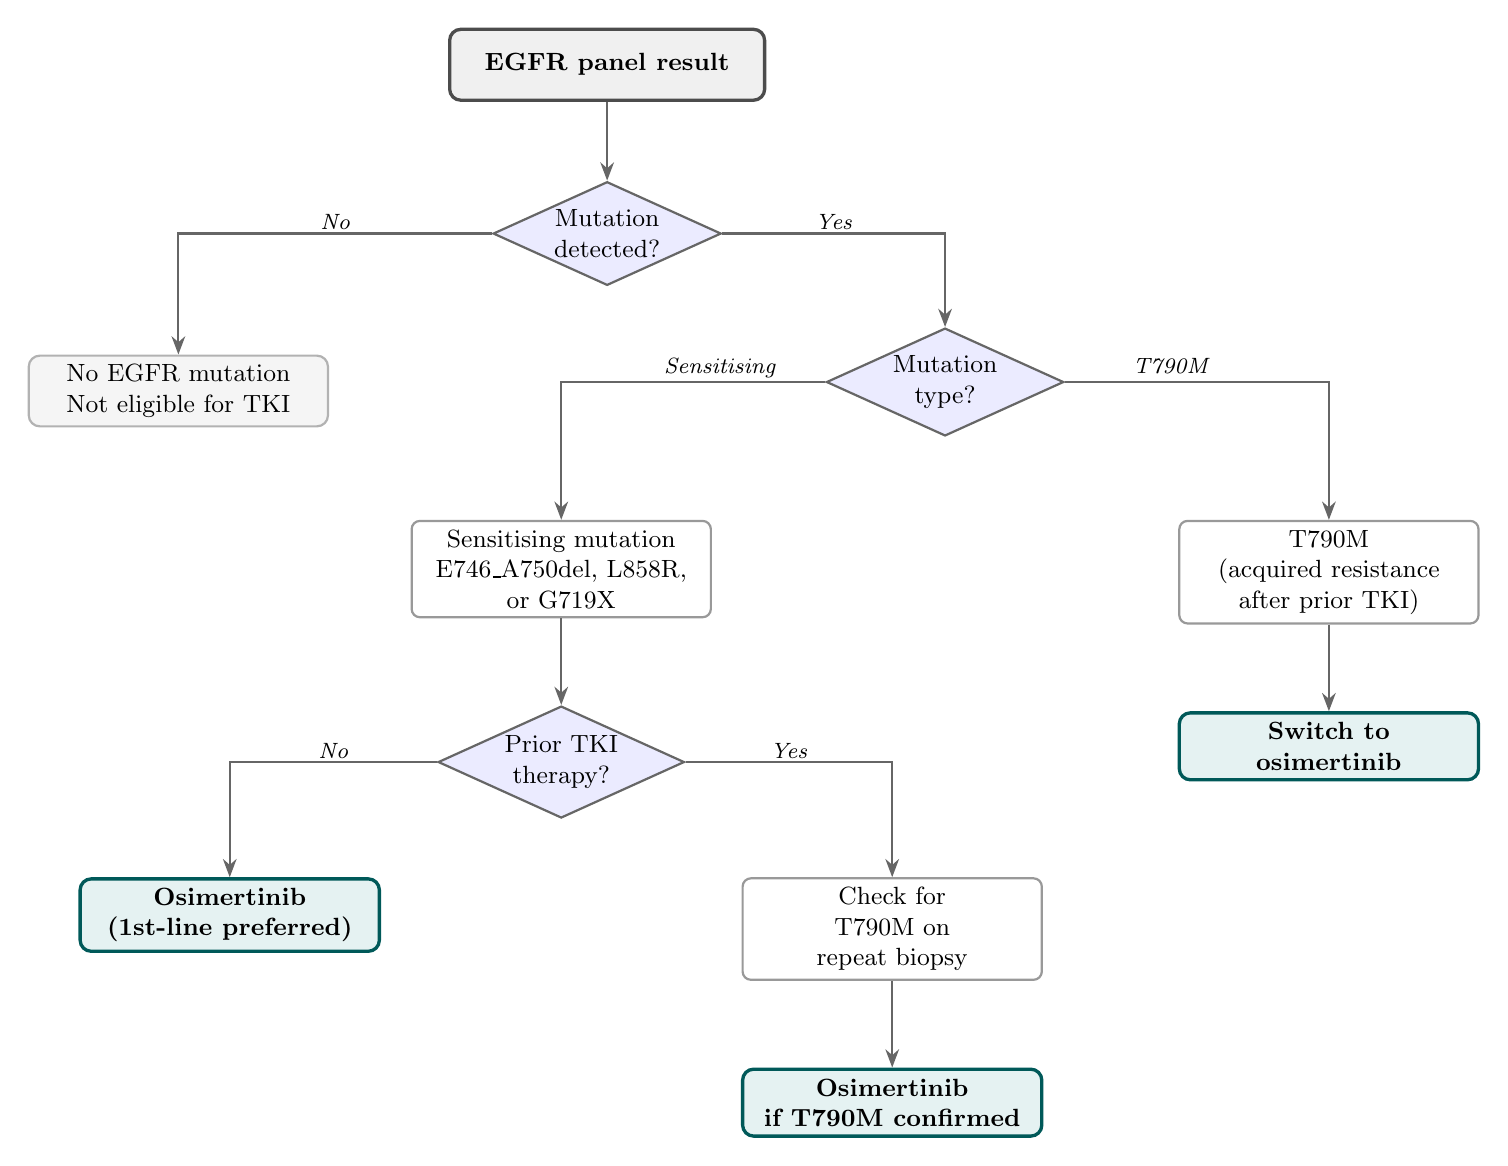
\begin{tikzpicture}[
  node distance = 0.6cm and 1.8cm,
  % Styles
  start/.style   = {rectangle, draw=black!70, very thick, fill=gray!12,
                    rounded corners=4pt, align=center, font=\small\bfseries,
                    minimum width=4cm, minimum height=0.9cm},
  decision/.style = {diamond, draw=black!60, thick, fill=blue!8,
                    align=center, font=\small, inner sep=1pt,
                    aspect=2.2},
  result/.style   = {rectangle, draw=black!40, thick, fill=white,
                    rounded corners=3pt, align=center, font=\small,
                    minimum width=3.8cm, minimum height=0.85cm},
  treat/.style    = {rectangle, draw=teal!70!black, very thick,
                    fill=teal!10, rounded corners=4pt, align=center,
                    font=\small\bfseries,
                    minimum width=3.8cm, minimum height=0.85cm},
  notreat/.style  = {rectangle, draw=gray!60, thick, fill=gray!8,
                    rounded corners=4pt, align=center, font=\small,
                    minimum width=3.8cm, minimum height=0.85cm},
  arrow/.style    = {->, >=Stealth, thick, draw=black!60},
  lbl/.style      = {font=\footnotesize\itshape, fill=white,
                    inner sep=1pt},
]

%% ── Nodes ──────────────────────────────────────────────────────────────────

% Root
\node[start] (panel) {EGFR panel result};

% Decision 1: mutation detected?
\node[decision, below=1.0cm of panel] (mut_q)
      {Mutation\\detected?};

% Left branch: no mutation
\node[notreat, below left=1.2cm and 2.8cm of mut_q] (no_mut)
      {No EGFR mutation\\Not eligible for TKI};

% Right branch: mutation detected → which type?
\node[decision, below right=1.2cm and 2.8cm of mut_q] (type_q)
      {Mutation\\type?};

% Sensitising branch (left of type_q)
\node[result, below left=1.4cm and 2.2cm of type_q] (sensitising)
      {Sensitising mutation\\E746\_A750del, L858R,\\or G719X};

% T790M branch (right of type_q)
\node[result, below right=1.4cm and 2.2cm of type_q] (t790m_node)
      {T790M\\(acquired resistance\\after prior TKI)};

% Treatment: sensitising → further question: naïve vs resistant?
\node[decision, below=1.1cm of sensitising] (naive_q)
      {Prior TKI\\therapy?};

\node[treat, below left=1.1cm and 1.5cm of naive_q] (osi_first)
      {Osimertinib\\(1st-line preferred)};

\node[result, below right=1.1cm and 1.5cm of naive_q] (check_t790m)
      {Check for\\T790M on\\repeat biopsy};

% Treatment: T790M → osimertinib
\node[treat, below=1.1cm of t790m_node] (osi_switch)
      {Switch to\\osimertinib};

% Treatment after repeat biopsy
\node[treat,  below=1.1cm of check_t790m] (osi_if)
      {Osimertinib\\if T790M confirmed};

%% ── Arrows ─────────────────────────────────────────────────────────────────

\draw[arrow] (panel)    -- (mut_q);

\draw[arrow] (mut_q)    -| node[lbl, above, pos=0.25] {No}  (no_mut);
\draw[arrow] (mut_q)    -| node[lbl, above, pos=0.25] {Yes} (type_q);

\draw[arrow] (type_q)   -| node[lbl, above, pos=0.2] {Sensitising} (sensitising);
\draw[arrow] (type_q)   -| node[lbl, above, pos=0.2] {T790M}       (t790m_node);

\draw[arrow] (sensitising) -- (naive_q);

\draw[arrow] (naive_q)  -| node[lbl, above, pos=0.25] {No}  (osi_first);
\draw[arrow] (naive_q)  -| node[lbl, above, pos=0.25] {Yes} (check_t790m);

\draw[arrow] (t790m_node) -- (osi_switch);
\draw[arrow] (check_t790m)  -- (osi_if);

\end{tikzpicture}
 inside a figure environment.

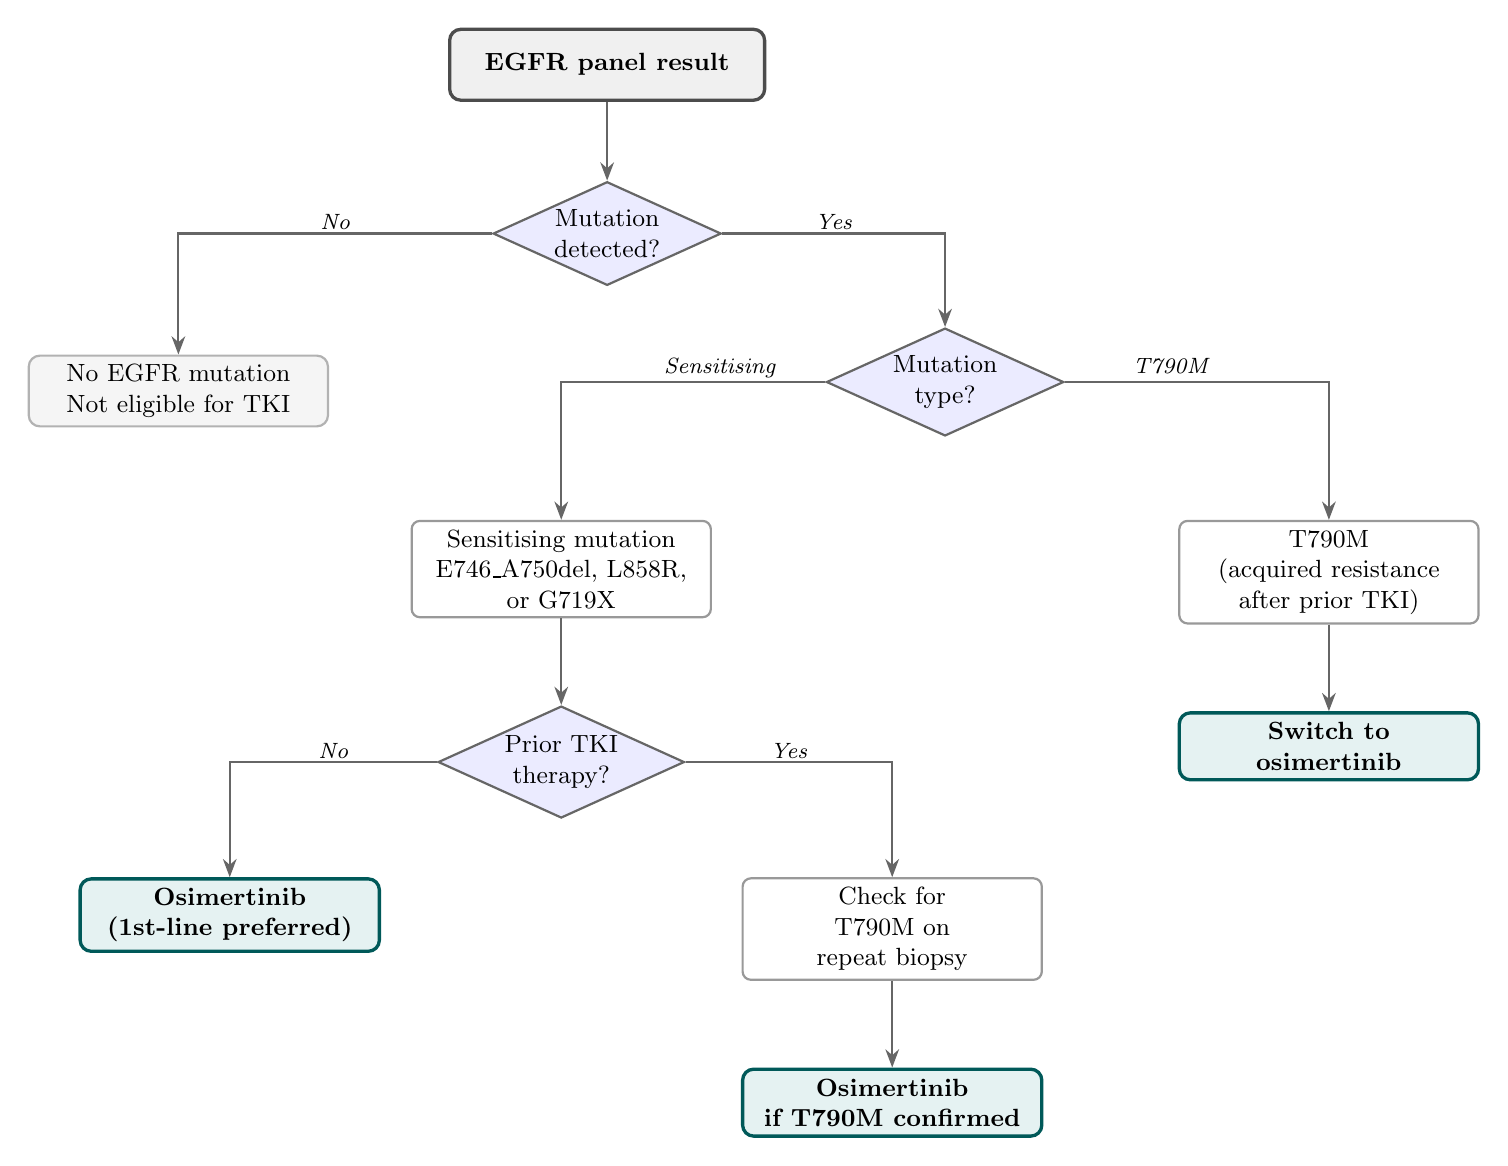
\begin{tikzpicture}[
  node distance = 0.6cm and 1.8cm,
  % Styles
  start/.style   = {rectangle, draw=black!70, very thick, fill=gray!12,
                    rounded corners=4pt, align=center, font=\small\bfseries,
                    minimum width=4cm, minimum height=0.9cm},
  decision/.style = {diamond, draw=black!60, thick, fill=blue!8,
                    align=center, font=\small, inner sep=1pt,
                    aspect=2.2},
  result/.style   = {rectangle, draw=black!40, thick, fill=white,
                    rounded corners=3pt, align=center, font=\small,
                    minimum width=3.8cm, minimum height=0.85cm},
  treat/.style    = {rectangle, draw=teal!70!black, very thick,
                    fill=teal!10, rounded corners=4pt, align=center,
                    font=\small\bfseries,
                    minimum width=3.8cm, minimum height=0.85cm},
  notreat/.style  = {rectangle, draw=gray!60, thick, fill=gray!8,
                    rounded corners=4pt, align=center, font=\small,
                    minimum width=3.8cm, minimum height=0.85cm},
  arrow/.style    = {->, >=Stealth, thick, draw=black!60},
  lbl/.style      = {font=\footnotesize\itshape, fill=white,
                    inner sep=1pt},
]

%% ── Nodes ──────────────────────────────────────────────────────────────────

% Root
\node[start] (panel) {EGFR panel result};

% Decision 1: mutation detected?
\node[decision, below=1.0cm of panel] (mut_q)
      {Mutation\\detected?};

% Left branch: no mutation
\node[notreat, below left=1.2cm and 2.8cm of mut_q] (no_mut)
      {No EGFR mutation\\Not eligible for TKI};

% Right branch: mutation detected → which type?
\node[decision, below right=1.2cm and 2.8cm of mut_q] (type_q)
      {Mutation\\type?};

% Sensitising branch (left of type_q)
\node[result, below left=1.4cm and 2.2cm of type_q] (sensitising)
      {Sensitising mutation\\E746\_A750del, L858R,\\or G719X};

% T790M branch (right of type_q)
\node[result, below right=1.4cm and 2.2cm of type_q] (t790m_node)
      {T790M\\(acquired resistance\\after prior TKI)};

% Treatment: sensitising → further question: naïve vs resistant?
\node[decision, below=1.1cm of sensitising] (naive_q)
      {Prior TKI\\therapy?};

\node[treat, below left=1.1cm and 1.5cm of naive_q] (osi_first)
      {Osimertinib\\(1st-line preferred)};

\node[result, below right=1.1cm and 1.5cm of naive_q] (check_t790m)
      {Check for\\T790M on\\repeat biopsy};

% Treatment: T790M → osimertinib
\node[treat, below=1.1cm of t790m_node] (osi_switch)
      {Switch to\\osimertinib};

% Treatment after repeat biopsy
\node[treat,  below=1.1cm of check_t790m] (osi_if)
      {Osimertinib\\if T790M confirmed};

%% ── Arrows ─────────────────────────────────────────────────────────────────

\draw[arrow] (panel)    -- (mut_q);

\draw[arrow] (mut_q)    -| node[lbl, above, pos=0.25] {No}  (no_mut);
\draw[arrow] (mut_q)    -| node[lbl, above, pos=0.25] {Yes} (type_q);

\draw[arrow] (type_q)   -| node[lbl, above, pos=0.2] {Sensitising} (sensitising);
\draw[arrow] (type_q)   -| node[lbl, above, pos=0.2] {T790M}       (t790m_node);

\draw[arrow] (sensitising) -- (naive_q);

\draw[arrow] (naive_q)  -| node[lbl, above, pos=0.25] {No}  (osi_first);
\draw[arrow] (naive_q)  -| node[lbl, above, pos=0.25] {Yes} (check_t790m);

\draw[arrow] (t790m_node) -- (osi_switch);
\draw[arrow] (check_t790m)  -- (osi_if);

\end{tikzpicture}
}
  \caption{Treatment decision tree based on EGFR panel result.
    Sensitising mutations (E746\_A750del, L858R, G719X) in treatment-na\"{i}ve
    patients lead directly to osimertinib~\cite{soria2018}.  Patients who progress on a
    prior TKI are re-tested for T790M; a confirmed T790M triggers a switch
    to osimertinib~\cite{mok2017}.}
  \label{fig:tki-decision}
\end{figure}

\paragraph{Mutations targeted by this panel.}
The four amplicons in this panel each target one exon of the EGFR kinase
domain, collectively covering the four most clinically relevant mutation
classes (Table~\ref{tab:egfr-hotspots}).

\begin{table}[H]
  \centering
  \caption{Clinically relevant EGFR mutations targeted by this panel, with
    their exon location, covering amplicon, and clinical role in NSCLC.
    Freq.: percentage of EGFR-mutant NSCLC patients carrying each mutation~\cite{lynch2004};
    the T790M figure applies to patients who have progressed on a prior TKI,
    as it is an acquired resistance mutation not present at diagnosis.
    Cross-reference with Table~\ref{tab:variants} for detected variants.}
  \label{tab:egfr-hotspots}
  \begin{tabular}{llllp{6cm}}
    \toprule
    \textbf{Mutation} & \textbf{Exon} & \textbf{Amplicon} & \textbf{Freq.} & \textbf{Clinical role} \\
    \midrule
    G719X         & 18 & 2 & $\sim$3\%  & Sensitising; responds to afatinib and osimertinib \\
    E746\_A750del & 19 & 1 & $\sim$45\% & Most common sensitising mutation; responds to all TKI generations \\
    T790M         & 20 & 4 & $\sim$50\% & Acquired resistance to 1st/2nd-gen TKIs; sensitises to osimertinib \\
    L858R         & 21 & 3 & $\sim$40\% & Second most common sensitising mutation; responds to all TKI generations \\
    \bottomrule
  \end{tabular}
\end{table}

\paragraph{EGFR-mutant NSCLC cell lines.}
The four EGFR hotspot mutations are each well-represented by established
non-small-cell lung cancer cell line models, which are widely used for
drug-sensitivity testing and as sequencing controls
(Table~\ref{tab:cell-lines}).
Each line carries a defined EGFR genotype, making them useful reference
standards: a sequencing run on a known cell line mix can be used to validate
that a panel detects the expected mutations at the expected allele frequencies.

\begin{table}[H]
  \centering
  \caption{EGFR mutation status of commonly used NSCLC cell lines for the
    four hotspots targeted by this panel.
    $\checkmark$ = mutation present; --- = wild-type at that position.
    The profile of our sample (E746\_A750del only, T790M/L858R absent)
    matches PC9 and HCC827.}
  \label{tab:cell-lines}
  \begin{tabular}{lllll}
    \toprule
    \textbf{Cell line} & \textbf{G719X} & \textbf{E746\_A750del} & \textbf{T790M} & \textbf{L858R} \\
    \midrule
    PC9       & --- & $\checkmark$ & --- & --- \\
    HCC827    & --- & $\checkmark$ & --- & --- \\
    H1975     & --- & ---          & $\checkmark$ & $\checkmark$ \\
    H3255     & --- & ---          & --- & $\checkmark$ \\
    NCI-H1650 & --- & $\checkmark$ & --- & --- \\
    A549      & --- & ---          & --- & --- \\
    \bottomrule
  \end{tabular}
  \par\smallskip
  \raggedright\small
  A549 is EGFR wild-type (KRAS G12S) and serves as a TKI-insensitive negative
  control.
  H1975 is the canonical model for acquired T790M resistance, as it expresses
  both the primary sensitising mutation (L858R) and the resistance mutation
  (T790M) simultaneously.
  PC9 and HCC827 both carry the most common exon~19 deletion (E746\_A750del)
  and are highly sensitive to all generations of EGFR TKIs.
\end{table}

\paragraph{Canonical genomic coordinates (hg19).}
Table~\ref{tab:egfr-coords} lists the precise reference coordinates for each
mutation class.
The nucleotide changes are given in VCF convention (plus-strand reference
allele first), consistent with the output of Mutect2 and VarDictJava.
These coordinates allow manual verification: querying the relevant position in
UCSC Genome Browser (hg19 assembly) or IGV should show the
expected reference base, and the variant can be confirmed by inspecting the
aligned reads in \texttt{aln.bam}.

\begin{table}[H]
  \centering
  \caption{Canonical hg19 genomic coordinates of the EGFR mutations targeted by
    this panel, sourced from COSMIC~\cite{tate2019} and
    ClinVar~\cite{landrum2018}.
    Ref/Alt follow VCF convention (plus-strand reference).
    G719X encompasses several codon-719 substitutions; the most common,
    G719S (COSM6252), is listed.}
  \label{tab:egfr-coords}
  \resizebox{\textwidth}{!}{%
  \begin{tabular}{lllllll}
    \toprule
    \textbf{Mutation}\textsuperscript{$a$} & \textbf{Exon} & \textbf{Chr} & \textbf{Position (hg19)} & \textbf{Ref} & \textbf{Alt} & \textbf{HGVS notation}\textsuperscript{$b$} \\
    \midrule
    G719S (G719X)  & 18 & 7 & 55,241,707 & \texttt{C} & \texttt{T} & \texttt{p.Gly719Ser} \\
    E746\_A750del  & 19 & 7 & 55,242,465 & \texttt{GGAATTAAGAGAAGCA} & \texttt{G} & \texttt{p.Glu746\_Ala750del} \\
    T790M          & 20 & 7 & 55,249,071 & \texttt{C} & \texttt{T} & \texttt{p.Thr790Met} \\
    L858R          & 21 & 7 & 55,259,515 & \texttt{T} & \texttt{G} & \texttt{p.Leu858Arg} \\
    \bottomrule
  \end{tabular}%
  }
  \par\smallskip
  \raggedright\small
  \textsuperscript{$a$}\textbf{Clinical shorthand} uses single-letter amino acid
  codes (e.g.\ E = Glu, A = Ala, T = Thr, L = Leu),
  as used in COSMIC and the oncology literature.
  \textsuperscript{$b$}\textbf{HGVS notation} uses three-letter amino acid codes
  (e.g.\ Glu, Ala, Thr, Leu), the internationally standardised format used by
  SnpEff and ClinVar; see Table~\ref{tab:variants} for the SnpEff-annotated calls.

  \medskip
  COSMIC identifiers: E746\_A750del = COSM6223; L858R = COSM6224\@.
  Note: both callers returned a PASS call at position 55,249,063
  (G$\rightarrow$A, 8\,bp upstream of T790M), annotated by SnpEff as the
  synonymous SNP \texttt{p.Gln787Gln} (dbSNP rs1050171) --- a common germline
  polymorphism, not a somatic driver (see Section~\ref{sec:variants-results}).
\end{table}

% ============================================================
\section{Background: Amplicon Sequencing}
\label{sec:background}
% ============================================================

\subsection{Workflow}

Amplicon sequencing is a targeted NGS strategy in which only predefined genomic loci are
sequenced~\cite{goodwin2016}. The workflow has four steps:

\begin{enumerate}
    \item \textbf{PCR amplification} --- primers flanking the regions of interest selectively
          amplify those loci, producing many copies (\emph{amplicons}) of each target.
    \item \textbf{Adaptor ligation} --- short synthetic adaptors are ligated to the PCR
          products, enabling flow-cell binding and cluster generation.
    \item \textbf{Sequencing by synthesis (SBS)} --- fluorescently labelled, reversible
          terminator nucleotides\footnote{Each of the four bases (A, T, C, G) carries a
          distinct coloured dye so the camera can identify which base was just added.
          The ``reversible terminator'' chemical group blocks the strand from growing further
          until it is removed, ensuring exactly one base is incorporated per imaging cycle.}
          are incorporated one at a time; a camera records which base
          was added at each cluster position per cycle.
    \item \textbf{Base calling} --- fluorescence images are decoded into FASTQ sequences with
          per-base Phred quality scores.
\end{enumerate}

Because all sequencing capacity is focused on a tiny fraction of the genome, depths of
$1{,}000$--$100{,}000\times$ are routine, enabling detection of somatic mutations at
$<$1\% VAF that would be invisible at typical WGS depths ($\sim$30--100$\times$).
The trade-off is that only the designed targets are assayed --- no off-target information
is captured, and prior knowledge of the variants of interest is required.

In this dataset, four amplicons cover EGFR hotspot exons 18--21, a design typical of
\textbf{oncology panels} used to detect driver mutations in lung cancer.

\subsection{Read Structure}

Each read from an amplicon library consists of three elements (Figure~\ref{fig:read-structure}):

\begin{description}
    \item[Adaptor] Synthetic oligonucleotide ligated to both fragment ends; enables flow-cell
        binding. Adaptors are not part of the biological sample and must be \emph{trimmed}
        before analysis. This library uses two adaptors:
        \texttt{AAGACTCGGCAGCATCTCCA} and \texttt{GCGATCGTCACTGTTCTCCA}.

    \item[Primer] Defines the amplicon boundaries; appears at the 5' end of R1 (forward) and
        R2 (reverse). Primers are trimmed or soft-clipped\footnote{%
          \textit{Soft-clipping} (CIGAR code \texttt{S}) is a BAM alignment
          operation in which the aligner retains the full read sequence in the
          file but marks the primer bases as not contributing to the alignment
          score or the pileup, so they do not influence variant calls at those
          positions.} before variant calling to avoid boundary artefacts. Four primer pairs target one amplicon each
        (Table~\ref{tab:primers}).

    \item[Amplified region] The biological sequence of interest between the primers, carrying
        any variants subject to downstream analysis.
\end{description}

The expected read layout is:
\begin{center}
    \texttt{[Adaptor]\;$\rightarrow$\;[Fwd Primer]\;$\rightarrow$\;[Amplified Region]\;$\rightarrow$\;[Rev Primer$_{RC}$]\;$\rightarrow$\;[Adaptor$_{RC}$]}
\end{center}

For short amplicons on a 2$\times$250\,bp MiSeq run, paired reads may overlap or read
into the opposite adaptor, making adapter trimming especially important~\cite{illumina_miseq}.

\begin{figure}[H]
\centering
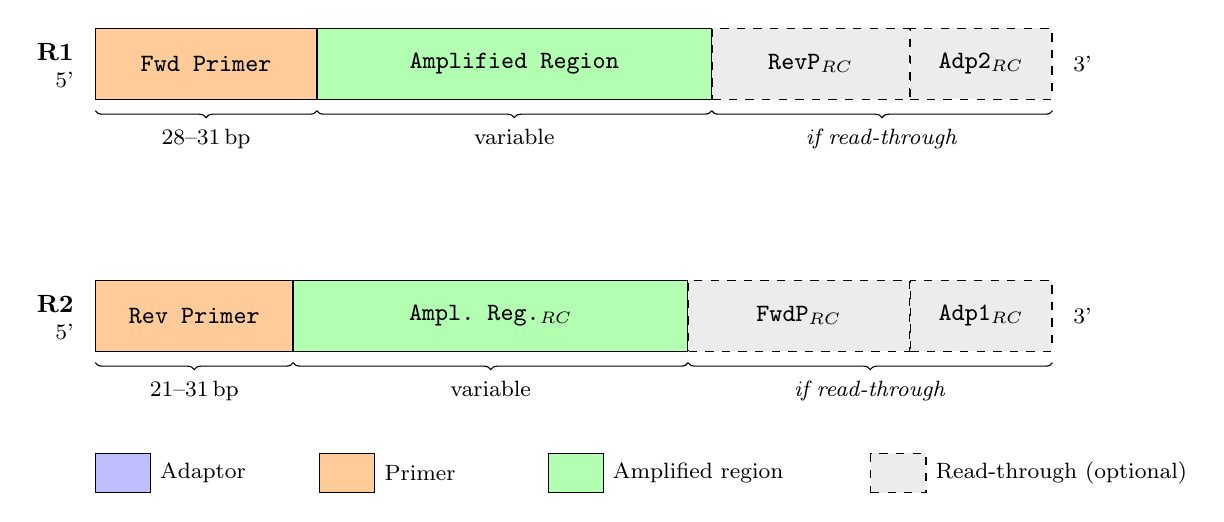
\begin{tikzpicture}[
    box/.style={draw, minimum height=0.9cm, text centered,
                font=\small\ttfamily, inner sep=3pt},
    adp/.style={box, fill=blue!25},
    prm/.style={box, fill=orange!40},
    amp/.style={box, fill=green!30},
    rth/.style={box, dashed, fill=gray!15},
    lbl/.style={font=\footnotesize},
]

% -------------------------------------------------------
% READ 1  (adapter is the priming site; read begins at forward primer)
% -------------------------------------------------------
\node[prm, minimum width=2.8cm, anchor=west] (r1fp) at (0, 0)     {Fwd Primer};
\node[amp, minimum width=5.0cm, anchor=west] (r1ar) at (r1fp.east){Amplified Region};
\node[rth, minimum width=2.5cm, anchor=west] (r1rp) at (r1ar.east){RevP$_{RC}$};
\node[rth, minimum width=1.8cm, anchor=west] (r1a2) at (r1rp.east){Adp2$_{RC}$};

% R1 label + direction
\node[anchor=east, font=\small\bfseries] at (-0.15, 0.15)  {R1};
\node[anchor=east, lbl]                  at (-0.15, -0.2)  {5'};
\node[anchor=west, lbl]                  at ([xshift=4pt]r1a2.east) {3'};

% Size annotations below R1
\draw[decorate, decoration={brace, mirror, raise=4pt}]
    (r1fp.south west) -- (r1fp.south east)
    node[midway, below=7pt, lbl] {28--31\,bp};
\draw[decorate, decoration={brace, mirror, raise=4pt}]
    (r1ar.south west) -- (r1ar.south east)
    node[midway, below=7pt, lbl] {variable};
\draw[decorate, decoration={brace, mirror, raise=4pt}]
    (r1rp.south west) -- (r1a2.south east)
    node[midway, below=7pt, lbl, text width=2.5cm, align=center]
        {\textit{if read-through}};

% -------------------------------------------------------
% READ 2  (adapter is the priming site; read begins at reverse primer)
% -------------------------------------------------------
\node[prm, minimum width=2.5cm, anchor=west] (r2rp) at (0, -3.2)    {Rev Primer};
\node[amp, minimum width=5.0cm, anchor=west] (r2ar) at (r2rp.east)  {Ampl.\ Reg.$_{RC}$};
\node[rth, minimum width=2.8cm, anchor=west] (r2fp) at (r2ar.east)  {FwdP$_{RC}$};
\node[rth, minimum width=1.8cm, anchor=west] (r2a1) at (r2fp.east)  {Adp1$_{RC}$};

% R2 label + direction
\node[anchor=east, font=\small\bfseries] at (-0.15, -3.05) {R2};
\node[anchor=east, lbl]                  at (-0.15, -3.4)  {5'};
\node[anchor=west, lbl]                  at ([xshift=4pt]r2a1.east) {3'};

% Size annotations below R2
\draw[decorate, decoration={brace, mirror, raise=4pt}]
    (r2rp.south west) -- (r2rp.south east)
    node[midway, below=7pt, lbl] {21--31\,bp};
\draw[decorate, decoration={brace, mirror, raise=4pt}]
    (r2ar.south west) -- (r2ar.south east)
    node[midway, below=7pt, lbl] {variable};
\draw[decorate, decoration={brace, mirror, raise=4pt}]
    (r2fp.south west) -- (r2a1.south east)
    node[midway, below=7pt, lbl, text width=2.5cm, align=center]
        {\textit{if read-through}};

% -------------------------------------------------------
% Legend
% -------------------------------------------------------
\begin{scope}[shift={(0, -5.2)}]
    \node[adp, minimum width=0.7cm, minimum height=0.5cm] (la) at (0.35, 0) {};
    \node[anchor=west, font=\footnotesize] at (0.7,  0) {Adaptor};

    \node[prm, minimum width=0.7cm, minimum height=0.5cm] (lp) at (3.2, 0) {};
    \node[anchor=west, font=\footnotesize] at (3.55, 0) {Primer};

    \node[amp, minimum width=0.7cm, minimum height=0.5cm] (lar) at (6.1, 0) {};
    \node[anchor=west, font=\footnotesize] at (6.45, 0) {Amplified region};

    \node[rth, minimum width=0.7cm, minimum height=0.5cm] (lrt) at (10.2, 0) {};
    \node[anchor=west, font=\footnotesize] at (10.55, 0) {Read-through (optional)};
\end{scope}

\end{tikzpicture}
\caption{Expected structure of paired-end reads from MiSeq amplicon
sequencing~\cite{illumina_miseq, goodwin2016}.
The sequencing primer binds\footnote{\textit{Annealing}: a short single-stranded
DNA oligonucleotide (the primer) binds to a complementary sequence on the template
strand via hydrogen bonds, positioning the polymerase to start copying from that
exact location.} within the adapter (Adp1 for R1, Adp2 for R2),
so the adapter itself is \emph{not} part of the sequenced read; sequencing begins
at the forward (R1) or reverse (R2) primer.
Solid borders: segments always present.
Dashed borders: segments that appear only when the read is long enough to
sequence through the full insert (read-through).
$_{RC}$: reverse complement.}
\label{fig:read-structure}
\end{figure}


% ============================================================
\section{Dataset Description}
\label{sec:dataset}
% ============================================================

This section documents the input files and library design parameters that were
provided with the task, and characterises the upstream processing history
extracted from the BAM file header.

\subsection{Provided Files}

Three files were provided:
\begin{itemize}
    \item \textbf{\texttt{aln.bam}} --- a pre-aligned BAM file mapped to the hg19
          reference genome using NCBI-style chromosome names (e.g.\ \texttt{7}
          instead of \texttt{chr7}).
    \item \textbf{\texttt{R1.fastq.gz}} --- raw paired-end reads, Read~1 (forward strand).
    \item \textbf{\texttt{R2.fastq.gz}} --- raw paired-end reads, Read~2 (reverse strand).
\end{itemize}

\subsection{Primer and Adaptor Sequences}

The following primer pairs and adaptor sequences were provided with the task and define
the library structure of each read (see Figure~\ref{fig:read-structure}).

\begin{table}[H]
\centering
\small
\resizebox{\textwidth}{!}{%
\begin{tabular}{clll}
\toprule
\textbf{Amplicon} & \textbf{Forward Primer (5'$\to$3')} & \textbf{Reverse Primer (5'$\to$3')} \\
\midrule
1 & \texttt{TTGCCAGTTAACGTCTTCCTTCTCTCTCTG} & \texttt{GAGAAAAGGTGGGCCTGAGGTTCAGAGCCA} \\
2 & \texttt{CCCTTGTCTCTGTGTTCTTGTCCCCCCCA}  & \texttt{CCCCACCAGACCATGAGAGGCCCTGCGGCC} \\
3 & \texttt{TGATCTGTCCCTCACAGCAGGGTCTTCTCT} & \texttt{TGACCTAAAGCCACCTCCTTA} \\
4 & \texttt{CACACTGACGTGCCTCTCCCTCCCTCCA}   & \texttt{CCGTATCTCCCTTCCCTGATTA} \\
\bottomrule
\end{tabular}%
}
\caption{Primer pairs defining the four EGFR amplicons. Reverse primers are given in
5'$\to$3' orientation (i.e.\ their reverse complement appears at the 3' end of R1
reads for short inserts — read-through events).}
\label{tab:primers}
\end{table}

\begin{table}[H]
\centering
\begin{tabular}{cll}
\toprule
\textbf{Adaptor} & \textbf{Sequence (5'$\to$3')} & \textbf{Length} \\
\midrule
Adaptor 1 & \texttt{AAGACTCGGCAGCATCTCCA} & 20\,bp \\
Adaptor 2 & \texttt{GCGATCGTCACTGTTCTCCA} & 20\,bp \\
\bottomrule
\end{tabular}
\caption{Custom adaptor sequences used in this dataset. Adaptor~1 is ligated to
the 5' end of the insert; the Read~1 sequencing primer anneals within Adaptor~1
so the sequenced read begins with the forward primer, not the adaptor itself.
Adaptor~2 is ligated to the opposite end and serves as the priming site for R2.
The reverse complements of these adaptors appear in reads only upon read-through
(Table~\ref{tab:adaptor-check}).}
\label{tab:adaptors}
\end{table}

\subsection{BAM Header Analysis}
\label{sec:bam-header}

A BAM file\footnote{BAM (Binary Alignment Map) is the compressed binary form of the
SAM (Sequence Alignment Map) format, the standard format for storing aligned sequencing
reads.} contains a plain-text header preceding the read data.
The header is organised into typed records, each beginning with a two-letter tag:

\begin{description}
    \item[\texttt{@HD}] File-level metadata: SAM format version and sort order
          (\texttt{SO:unsorted} here, meaning reads are not sorted by coordinate).
    \item[\texttt{@SQ}] Reference sequence dictionary: one entry per chromosome,
          giving the name and length used during alignment.
          This confirms the reference genome (hg19) and naming convention.
    \item[\texttt{@RG}] Read group: sample identifier, sequencing platform, and
          library information.
          Here: \texttt{ID:Bordet\_EGFR\_S1}, \texttt{SM:S1}, \texttt{PL:Illumina}.
    \item[\texttt{@PG}] Program record: the processing history of the file ---
          which programs were run, in which order, with which version, and
          (where available) the exact command line used.
\end{description}

The \texttt{@PG} and \texttt{@RG} lines of this BAM are:

\begin{lstlisting}
@RG  ID:Bordet_EGFR_S1  SM:S1  PL:Illumina
@PG  ID:bowtie2  PN:bowtie2  VN:2.0.2
\end{lstlisting}

This reveals three important facts:
\begin{itemize}
    \item The reads were aligned with \textbf{bowtie2} (v2.0.2).
    \item \textbf{No adaptor trimming step is recorded} in the processing history.
          The raw FASTQs were passed directly to the aligner without prior Cutadapt
          or equivalent preprocessing.
    \item \textbf{No primer trimming step is recorded.}
          In a standard amplicon sequencing pipeline, \texttt{ivar trim} (or an
          equivalent tool) is run after alignment to soft-clip the PCR primer
          sequences from the 5' end of each read using a BED file of primer
          coordinates. This prevents the synthetic primer bases from entering the
          variant-calling pileup: because primer sequences are identical across
          every molecule from a given amplicon, any mismatch between the primer
          and the reference genome will appear as a near-100\% VAF ``variant'' at
          the amplicon boundary --- a primer-end artefact rather than a true somatic
          mutation. The absence of an \texttt{ivar trim} \texttt{@PG} entry
          confirms this step was skipped, with direct consequences for variant
          calling at amplicon boundaries (Section~\ref{sec:variants-results}).
\end{itemize}

The consequence for adapter contamination is that reads containing adaptor sequence
at their 3' end were aligned as-is; bowtie2 would have soft-clipped those bases,
which may slightly reduce effective coverage at amplicon boundaries.
Our Cutadapt run (Section~\ref{sec:read-constitution}) is therefore a purely
retrospective QC characterisation and did not feed into the alignment.

The BAM header can be reproduced with the Snakemake rule \texttt{bam\_header}:

\begin{lstlisting}[language=bash]
bash pipeline/run.sh --cores 4 --until bam_header
# Output: pipeline/results/qc/bam_header.txt
\end{lstlisting}

% ============================================================
\section{Read Quality and Constitution}
\label{sec:read-constitution}
% ============================================================

\textbf{Question:} What is the constitution of each read, for example (adaptor + primer + amplified region)?

Before characterising the specific structure of each read, we first verify that the raw
data is of sufficient quality to analyse at all.
General quality metrics (base quality, GC content, duplication) are independent of the
library design and serve as a prerequisite sanity check — if the sequencing run itself
failed, the downstream read constitution analysis would be meaningless.
Only after confirming data quality do we proceed to examine the specific read layout
using the known primer and adaptor sequences.

% ------------------------------------------------------------
\subsection{Raw Read Quality Assessment}
\label{sec:raw-quality}
% ------------------------------------------------------------

\subsubsection{Methods}

FastQC~\cite{andrews2010} was run on the raw FASTQ files to assess overall read
quality — base quality scores, GC content distribution, sequence length distribution,
duplication levels, and adaptor content flags — before any library-specific analysis.
FastQC was subsequently re-run on the adapter-trimmed reads as a before/after check.

\begin{lstlisting}[language=bash]
bash pipeline/run.sh --cores 4 --until task1_fastqc_table
\end{lstlisting}

\subsubsection{Results}

Figure~\ref{fig:ngs-pipeline} shows the role of each tool in a standard NGS preprocessing pipeline.

\begin{figure}[H]
\centering
\resizebox{\textwidth}{!}{%
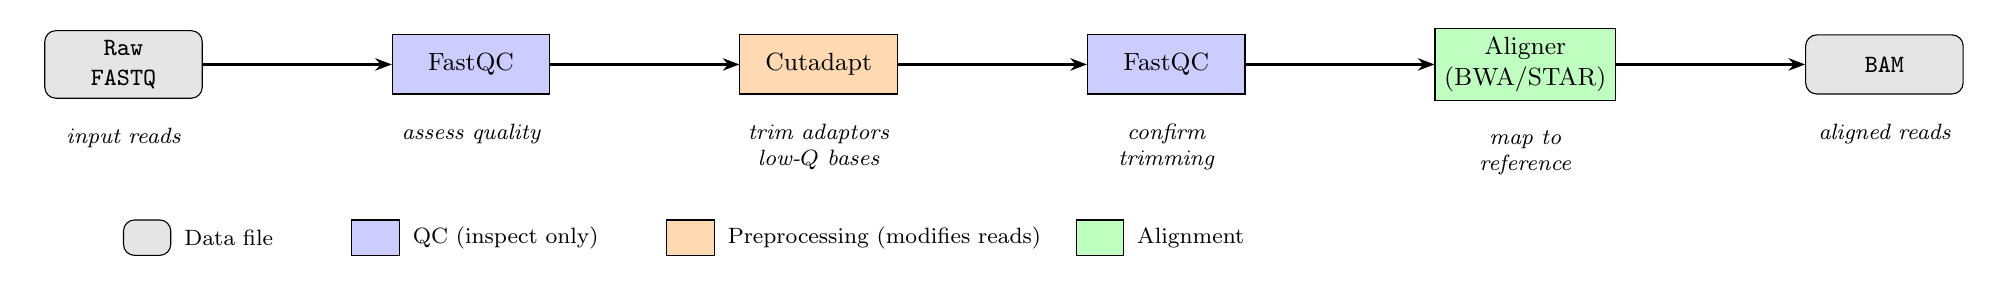
\begin{tikzpicture}[
    node distance=2.4cm,
    % Data files: rounded gray boxes
    data/.style={
        draw, rounded corners=4pt, fill=gray!20,
        minimum width=2.0cm, minimum height=0.75cm,
        font=\small\ttfamily, align=center
    },
    % QC tools: blue boxes
    qc/.style={
        draw, fill=blue!20,
        minimum width=2.0cm, minimum height=0.75cm,
        font=\small, align=center
    },
    % Preprocessing tools: orange boxes
    preproc/.style={
        draw, fill=orange!30,
        minimum width=2.0cm, minimum height=0.75cm,
        font=\small, align=center
    },
    % Alignment: green boxes
    aligner/.style={
        draw, fill=green!25,
        minimum width=2.0cm, minimum height=0.75cm,
        font=\small, align=center
    },
    lbl/.style={font=\footnotesize\itshape, align=center, text width=2.2cm},
    arr/.style={-{Stealth[length=6pt]}, thick},
]

% ---- Nodes ----
\node[data]    (fastq)    {Raw\\FASTQ};
\node[qc]      (fqc1)     [right=of fastq]    {FastQC};
\node[preproc] (cutadapt) [right=of fqc1]     {Cutadapt};
\node[qc]      (fqc2)     [right=of cutadapt] {FastQC};
\node[aligner] (aligner)  [right=of fqc2]     {Aligner\\(BWA/STAR)};
\node[data]    (bam)      [right=of aligner]   {BAM};

% ---- Arrows ----
\draw[arr] (fastq)    -- (fqc1);
\draw[arr] (fqc1)     -- (cutadapt);
\draw[arr] (cutadapt) -- (fqc2);
\draw[arr] (fqc2)     -- (aligner);
\draw[arr] (aligner)  -- (bam);

% ---- Labels below each node ----
\node[lbl, below=0.25cm of fastq]    {input reads};
\node[lbl, below=0.25cm of fqc1]    {assess quality};
\node[lbl, below=0.25cm of cutadapt]{trim adaptors\\low-$Q$ bases};
\node[lbl, below=0.25cm of fqc2]    {confirm\\trimming};
\node[lbl, below=0.25cm of aligner] {map to\\reference};
\node[lbl, below=0.25cm of bam]     {aligned reads};

% ---- Legend ----
\begin{scope}[shift={(0, -2.2)}]
    \node[data,    minimum width=0.6cm, minimum height=0.45cm] (ld) at (0.3,   0) {};
    \node[anchor=west, font=\footnotesize] at (0.65, 0) {Data file};

    \node[qc,      minimum width=0.6cm, minimum height=0.45cm] (lq) at (3.2,   0) {};
    \node[anchor=west, font=\footnotesize] at (3.55, 0) {QC (inspect only)};

    \node[preproc, minimum width=0.6cm, minimum height=0.45cm] (lp) at (7.2,   0) {};
    \node[anchor=west, font=\footnotesize] at (7.55, 0) {Preprocessing (modifies reads)};

    \node[aligner, minimum width=0.6cm, minimum height=0.45cm] (la) at (12.4,  0) {};
    \node[anchor=west, font=\footnotesize] at (12.75, 0) {Alignment};
\end{scope}

\end{tikzpicture}%
}% end resizebox
\caption{Typical NGS preprocessing pipeline before alignment.
\textbf{FastQC} (blue) is a quality control tool --- it inspects and reports read
quality but does not modify any data.
\textbf{Cutadapt} (orange) is a \emph{preprocessing} tool --- its primary purpose
is to remove adaptor sequences and trim low-quality bases \emph{before alignment},
so that the aligner receives clean reads and produces accurate mappings.
A second FastQC run after trimming confirms that the cleaning was successful.
In this dataset the BAM file was provided pre-aligned, so Cutadapt was run
retrospectively on the raw FASTQs to confirm adaptor presence and measure
insert size, rather than as a mandatory preprocessing step before mapping.}
\label{fig:ngs-pipeline}
\end{figure}


\subsubsection*{FastQC: Read Quality and Contamination Assessment}
\label{sec:fastqc-results}

FastQC was run on both raw\footnote{%
    \emph{Raw reads} are the reads exactly as produced by the sequencer, before
    any processing. They contain the full sequence including adaptors, primers,
    low-quality bases, and the amplified insert.}
and adapter-trimmed\footnote{%
    \emph{Adapter-trimmed reads} are reads after Cutadapt has removed adaptor
    sequences from the 3' end and clipped low-quality bases (Q$<$20).
    The biological insert (primer + amplified region) is left intact.
    Running FastQC on both raw and trimmed reads serves as a before/after check:
    adaptor warnings present before trimming should disappear afterwards,
    confirming that the correct sequences were specified and trimming worked
    as intended.}
reads; results are summarised in
Table~\ref{tab:fastqc}. All outputs are available in
\texttt{pipeline/\allowbreak results/\allowbreak qc/}.

% Auto-generated by pipeline/scripts/fastqc_table.py via rule task1_fastqc_table.
% To regenerate: bash pipeline/run.sh --cores 4 --until task1_fastqc_table
% then copy pipeline/results/tables/fastqc_table.tex here.
% Auto-generated by pipeline/scripts/fastqc_table.py — do not edit manually.
\begin{table}[H]
\centering
\begin{tabular}{lcccc}
\toprule
\textbf{Module} & \textbf{Raw R1} & \textbf{Raw R2} & \textbf{Trim R1} & \textbf{Trim R2} \\
\midrule
Basic Statistics & \textcolor{green!60!black}{\textbf{pass}} & \textcolor{green!60!black}{\textbf{pass}} & \textcolor{green!60!black}{\textbf{pass}} & \textcolor{green!60!black}{\textbf{pass}} \\
Per base sequence quality & \textcolor{green!60!black}{\textbf{pass}} & \textcolor{orange!80!black}{\textbf{warn}} & \textcolor{green!60!black}{\textbf{pass}} & \textcolor{green!60!black}{\textbf{pass}} \\
Per tile sequence quality & \textcolor{green!60!black}{\textbf{pass}} & \textcolor{green!60!black}{\textbf{pass}} & \textcolor{green!60!black}{\textbf{pass}} & \textcolor{green!60!black}{\textbf{pass}} \\
Per sequence quality scores & \textcolor{green!60!black}{\textbf{pass}} & \textcolor{green!60!black}{\textbf{pass}} & \textcolor{green!60!black}{\textbf{pass}} & \textcolor{green!60!black}{\textbf{pass}} \\
Per base sequence content & \textcolor{red}{\textbf{fail}}$^{*}$ & \textcolor{red}{\textbf{fail}}$^{*}$ & \textcolor{red}{\textbf{fail}}$^{*}$ & \textcolor{red}{\textbf{fail}}$^{*}$ \\
Per sequence GC content & \textcolor{red}{\textbf{fail}}$^{*}$ & \textcolor{red}{\textbf{fail}}$^{*}$ & \textcolor{red}{\textbf{fail}}$^{*}$ & \textcolor{red}{\textbf{fail}}$^{*}$ \\
Per base N content & \textcolor{green!60!black}{\textbf{pass}} & \textcolor{green!60!black}{\textbf{pass}} & \textcolor{green!60!black}{\textbf{pass}} & \textcolor{green!60!black}{\textbf{pass}} \\
Sequence Length Distribution & \textcolor{green!60!black}{\textbf{pass}} & \textcolor{green!60!black}{\textbf{pass}} & \textcolor{orange!80!black}{\textbf{warn}} & \textcolor{orange!80!black}{\textbf{warn}} \\
Sequence Duplication Levels & \textcolor{red}{\textbf{fail}}$^{*}$ & \textcolor{red}{\textbf{fail}}$^{*}$ & \textcolor{red}{\textbf{fail}}$^{*}$ & \textcolor{red}{\textbf{fail}}$^{*}$ \\
Overrepresented sequences & \textcolor{red}{\textbf{fail}}$^{*}$ & \textcolor{red}{\textbf{fail}}$^{*}$ & \textcolor{red}{\textbf{fail}}$^{*}$ & \textcolor{red}{\textbf{fail}}$^{*}$ \\
Adapter Content & \textcolor{green!60!black}{\textbf{pass}} & \textcolor{green!60!black}{\textbf{pass}} & \textcolor{green!60!black}{\textbf{pass}} & \textcolor{green!60!black}{\textbf{pass}} \\
\bottomrule
\multicolumn{5}{l}{\footnotesize $^{*}$ Expected artefact in amplicon sequencing --- not a quality concern (see text).} \\
\end{tabular}
\caption{FastQC quality-control summary for raw and adapter-trimmed reads. Fail flags marked $^{*}$ are expected artefacts of targeted amplicon sequencing and do not indicate a quality problem.}
\label{tab:fastqc}
\end{table}


The four \textbf{fail} flags marked with $^{*}$ are expected artefacts of amplicon
sequencing and do not indicate a quality problem:

\begin{itemize}
    \item \textbf{Per base sequence content:} FastQC expects a roughly equal A/T/G/C mix
          at each position. R1 always starts with the same forward primer ($\sim$30\,bp of
          fixed sequence), so the first bases show a strongly biased composition that
          FastQC flags as a fail. This is normal for any targeted amplicon library.
          To confirm this is purely a primer artefact, one could hard-clip\footnote{%
          \textit{Hard-clipping} (CIGAR code \texttt{H}) permanently removes bases
          from both the read sequence and the BAM record — unlike soft-clipping
          (\texttt{S}), which retains the bases in the file but excludes them from
          the alignment.  Hard-clipped bases are gone and cannot be recovered from
          the BAM.} the primer
          bases before running FastQC (e.g.\ using \texttt{iVar trim} with the amplicon
          BED file): if the fail disappears, the bias originated solely from the fixed
          primer sequence; if it persists, it would indicate genuine amplification bias
          in the insert sequence itself.
    \item \textbf{Per sequence GC content:} A whole-genome library produces a smooth
          bell-curve GC distribution centred on the genome average. Here only four
          specific amplicons are sequenced, each with its own fixed GC content,
          producing a multi-modal or shifted distribution.
          The per-primer GC content is analysed in detail in
          Section~\ref{sec:primer-properties}.
    \item \textbf{Sequence duplication levels:} PCR amplification generates many identical
          copies of the same molecule by design. High duplication is expected and
          intentional (deep coverage is the goal); it would only be a concern in WGS.
    \item \textbf{Overrepresented sequences:} Primer and amplicon sequences repeat
          thousands of times across reads by construction.
\end{itemize}

The modules that \emph{do} matter --- per-base quality, per-tile quality, per-sequence
quality scores, per-base N content, and adapter content --- are mostly clean, with two
non-critical observations:

\begin{itemize}
    \item \textbf{Per-base sequence quality, raw R2 (warn):} Phred scores decline at the
          3' end of R2, a common sequencing-by-synthesis artefact (later cycles accumulate
          more signal noise).
          Crucially, the BAM file provided was aligned from the \emph{raw} reads without a
          prior quality-trimming step (Section~\ref{sec:bam-header}), so these lower-quality
          bases are present in the alignment.
          All downstream variant callers apply a per-base quality threshold of $Q \geq 20$
          (VarDictJava \texttt{-q~20}, VarScan2 \texttt{--min-avg-qual~20}, samtools depth
          \texttt{-Q~20}), which excludes the worst bases.
          The warn resolves to pass after Cutadapt trimming, confirming that quality
          trimming before alignment would have fully mitigated this issue.
    \item \textbf{Sequence length distribution, trimmed reads (warn):} Adapter trimming
          produces reads of variable length (some reads are shorter after trimming), which
          FastQC flags whenever lengths are not uniform.
          This is expected behaviour and does not affect downstream analysis.
\end{itemize}

% ------------------------------------------------------------
\subsection{Read Constitution}
\label{sec:read-constitution-sub}
% ------------------------------------------------------------

\subsubsection{Methods}

Having confirmed the data quality, we characterise the specific structure of each read
using the primer and adaptor sequences documented in Section~\ref{sec:dataset}
(Tables~\ref{tab:primers} and~\ref{tab:adaptors}).
This addresses four practical questions:

\begin{enumerate}
    \item \textbf{Adaptor identification} --- which adaptor sequences flank the amplicons,
          and what is the correct trimming strategy?
    \item \textbf{Adaptor contamination} --- what fraction of reads contain read-through
          adaptor sequence at the 3' end?
    \item \textbf{Primer presence} --- do the primer sequences appear at the expected
          5' position in each read, confirming the amplification worked as designed?
    \item \textbf{Fragment length} --- what are the insert sizes per amplicon, and are
          they consistent with the amplicons being longer than the read length?
\end{enumerate}

The following steps were carried out:

\begin{enumerate}
    \item A custom script searched for all four adaptor sequences (Adp1, Adp1\textsubscript{RC},
          Adp2, Adp2\textsubscript{RC}) in the raw reads to identify which adaptors flank the
          amplicons and confirm the correct trimming sequences
          (Section~\ref{sec:adaptor-verification}).
    \item \textbf{Cutadapt}~\cite{martin2011} was run with the confirmed adaptor sequences to
          quantify adaptor contamination rates in the reads as a QC step
          (Section~\ref{sec:adaptor-verification}).
    \item Primer sequences were verified to be present at the expected 5' position of
          each read by primer-matching assignment
          (Section~\ref{sec:primer-verification}; per-amplicon read-through detail in
          Appendix~\ref{app:per-amplicon-readthrough}).
    \item Per-amplicon insert size distributions were extracted from the BAM TLEN field
          to confirm each amplicon's fragment length
          (Section~\ref{sec:insert-size}).
\end{enumerate}

\subsubsection{Adaptor verification: which adaptor appears in each read?}
\label{sec:adaptor-verification}

\paragraph{Where do adaptors appear in a read?}
Although every sequenced DNA molecule carries adaptors on \emph{both} ends, only the
\textbf{3' end} can contain adaptor sequence in the read itself
(see Figure~\ref{fig:read-structure} for the full read layout).
The 5' adaptor is the sequencing primer binding site --- sequencing starts from it, so it
is never incorporated into the read sequence.
The 3' adaptor (on the far end of the molecule) only appears in a read when the insert is
shorter than the read length: the sequencer reads through the entire amplicon and continues
into the far adaptor. This \emph{read-through} is therefore the sole source of adaptor
contamination, and it can only ever appear at the \textbf{3' end} of the read.

Two library configurations are possible depending on whether the same adaptor or two
distinct adaptors flank the amplicon (Figure~\ref{fig:adaptor-scenarios}).
Since this dataset provides \textbf{two distinct} adaptor sequences (Adp1 $\neq$ Adp2),
\textbf{Scenario~B} (different adaptors on each end) was assumed; this was subsequently
confirmed empirically (Appendix~\ref{app:adaptor-scenarios}).

\begin{figure}[H]
\centering
\resizebox{\textwidth}{!}{%
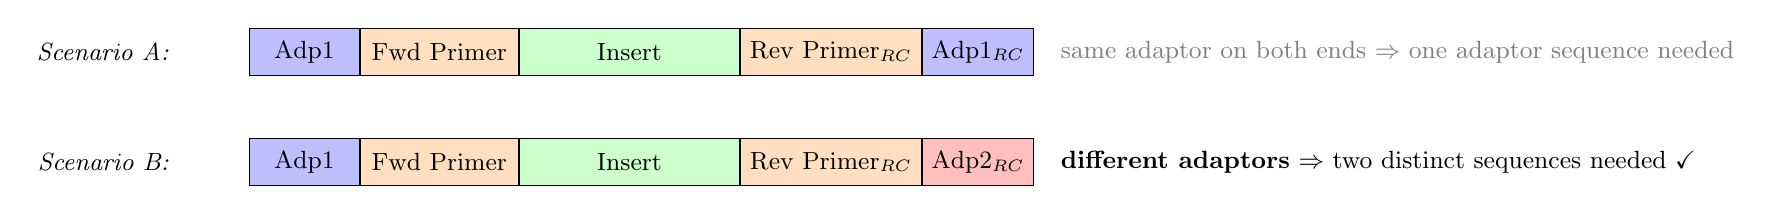
\begin{tikzpicture}[
    node distance=0pt,
    adp1/.style={draw, fill=blue!25, minimum width=1.4cm, minimum height=0.6cm,
                 font=\small, align=center},
    adp2/.style={draw, fill=red!25,  minimum width=1.4cm, minimum height=0.6cm,
                 font=\small, align=center},
    primer/.style={draw, fill=orange!25, minimum width=2.0cm, minimum height=0.6cm,
                   font=\small, align=center},
    ins/.style={draw, fill=green!20, minimum width=2.8cm, minimum height=0.6cm,
                font=\small, align=center},
    lbl/.style={font=\small\itshape, anchor=east},
]

% ---- Scenario A ----
\node[lbl] at (0, 1.4) {Scenario A:};
\node[adp1] (a1)   at (1.6,  1.4) {Adp1};
\node[primer, right=of a1]  (afp)  {Fwd Primer};
\node[ins,    right=of afp] (ains) {Insert};
\node[primer, right=of ains](arp)  {Rev Primer$_{RC}$};
\node[adp1,   right=of arp] (a1rc) {Adp1$_{RC}$};
\node[font=\small, gray, anchor=west] at ([xshift=6pt]a1rc.east)
    {same adaptor on both ends $\Rightarrow$ one adaptor sequence needed};

% ---- Scenario B ----
\node[lbl] at (0, 0) {Scenario B:};
\node[adp1] (b1)   at (1.6, 0) {Adp1};
\node[primer, right=of b1]  (bfp)  {Fwd Primer};
\node[ins,    right=of bfp] (bins) {Insert};
\node[primer, right=of bins](brp)  {Rev Primer$_{RC}$};
\node[adp2,   right=of brp] (b2rc) {Adp2$_{RC}$};
\node[font=\small, anchor=west] at ([xshift=6pt]b2rc.east)
    {\textbf{different adaptors} $\Rightarrow$ two distinct sequences needed \checkmark};

\end{tikzpicture}%
}
\caption{The two possible adaptor configurations for a paired-end amplicon library.
Scenario~A uses the same adaptor on both ends (one sequence suffices);
Scenario~B uses two distinct adaptors (two sequences required).
Since two distinct adaptor sequences (Adp1 $\neq$ Adp2) were provided with this dataset,
Scenario~B was assumed and subsequently confirmed empirically
(Appendix~\ref{app:adaptor-scenarios}).}
\label{fig:adaptor-scenarios}
\end{figure}


\paragraph{Is there adapter contamination?}
Adapter contamination refers to adapter sequences appearing within reads, which occurs
when the sequencer reads through the entire insert and into the far adapter.
A small fraction of contaminated reads is expected in any paired-end library and is
not a quality failure --- it simply indicates that those fragments are shorter than
the read length.
Using the Snakemake rule \texttt{task1\_check\_adaptors} (\texttt{bash pipeline/run.sh
--until task1\_check\_adaptors}), the script \texttt{check\_adaptors.py} searched for
all four sequences (Adp1, Adp1\textsubscript{RC}, Adp2, Adp2\textsubscript{RC}) in the
raw reads (Table~\ref{tab:adaptor-check}).
The results match expectations precisely:
\begin{itemize}
    \item \textbf{5' priming adaptors absent from reads.}
          Adp1 in R1\footnote{R1 (Read~1) and R2 (Read~2) are the two reads of a paired-end run, as defined in Section~\ref{sec:dataset}.} (0.682\%) and Adp2 in R2 ($\approx$0\%) are effectively absent, as
          expected --- they are the primer binding sites from which sequencing starts and
          are therefore never incorporated into the read sequence.
    \item \textbf{RC sequences present at the 3' end.}
          Adp2\textsubscript{RC} appears in 4.8\% of R1 reads and Adp1\textsubscript{RC}
          in 5.3\% of R2 reads --- the read-through signal from the far adaptor.
          This rate is consistent with the insert size distributions showing all four
          amplicons peak well above 150\,bp (Figure~\ref{fig:insert-size}).
          The asymmetry between R1 (4.8\%) and R2 (10.9\%) suggests that the reverse
          primer sits closer to the far adaptor than the forward primer --- a common
          consequence of primers being placed at different offsets relative to the
          region of interest.
\end{itemize}
The presence of \emph{different} RC signals in R1 and R2 (Adp2\textsubscript{RC} vs.\
Adp1\textsubscript{RC}) confirms \textbf{Scenario~B} (different adaptors on each end),
which determines the correct Cutadapt trimming flags used in Section~\ref{sec:cutadapt-summary}.
The correct trimming strategy is therefore to clip Adp2\textsubscript{RC} from the 3' end of R1
and Adp1\textsubscript{RC} from the 3' end of R2, as configured with Cutadapt's \texttt{-a}/\texttt{-A}
flags.

The full derivation of how the two scenarios produce distinguishable read-through
fingerprints, and how the script exploits this to confirm Scenario~B, is given in
Appendix~\ref{app:adaptor-scenarios}.

% Auto-generated by pipeline/scripts/adaptor_check_table.py — do not edit manually.
\begin{table}[H]
\centering
\begin{tabular}{llrrrr}
\toprule
\textbf{Label} & \textbf{Sequence (5'$\to$3')} & \textbf{R1 count} & \textbf{R1\,\%} & \textbf{R2 count} & \textbf{R2\,\%} \\
\midrule
\texttt{Adp1    (fwd)} & \texttt{AAGACTCGGCAGCATCTCCA} & 3,924 & 0.682\% & 0 & 0.000\% \\
\texttt{Adp2    (fwd)} & \texttt{GCGATCGTCACTGTTCTCCA} & 7 & 0.001\% & 2 & 0.000\% \\
\bottomrule
\end{tabular}
\caption{Occurrence of both adaptor sequences and their reverse complements (RC)
in R1 and R2 raw reads. Bold values indicate the dominant signal in each read.
Adp2~RC is dominant in R1 and Adp1~RC is dominant in R2, confirming
Scenario~B: the library uses different adaptors on each end (standard paired-end).}
\label{tab:adaptor-check}
\end{table}


\paragraph{Cutadapt trimming}\label{sec:cutadapt-summary}
Cutadapt is often used to remove adaptor contamination: it searches for the confirmed adaptor
sequences at the 3' end of each read and clips them, along with any low-quality bases.
The trimming rates (Table~\ref{tab:cutadapt}) directly quantify how many reads were
affected by read-through contamination.

% Auto-generated by pipeline/scripts/cutadapt_table.py via rule task1_cutadapt_table.
% To regenerate: bash pipeline/run.sh --cores 4 --until task1_cutadapt_table
% then copy pipeline/results/tables/cutadapt_table.tex here.
% Auto-generated by pipeline/scripts/cutadapt_table.py — do not edit manually.
\begin{table}[H]
\centering
\begin{tabular}{lrr}
\toprule
\textbf{Metric} & \textbf{Count} & \textbf{Fraction} \\
\midrule
Total read pairs processed & 575,002 &  \\
Read~1 with Adaptor~1 detected & 35,489 & (6.2\%) \\
Read~2 with Adaptor~2 detected & 62,613 & (10.9\%) \\
Pairs discarded (too short) & 1,983 & (0.3\%) \\
Pairs written (passing filters) & 573,019 & (99.7\%) \\
Total bases quality-trimmed & 2,122,235 & (1.2\%) \\
\bottomrule
\end{tabular}
\caption{Cutadapt~\cite{martin2011} adapter trimming summary for the paired-end MiSeq dataset.
  Adaptor~1 (\texttt{TGGAGAACAGTGACGATCGC}) trimmed from R1;
  Adaptor~2 (\texttt{TGGAGATGCTGCCGAGTCTT}) trimmed from R2.}
\label{tab:cutadapt}
\end{table}


Adapter detection rates of 6.2\% on R1 and 10.9\% on R2 indicate that the majority of reads
do \emph{not} read through into the opposite adapter. This confirms that most amplicons are
\textbf{longer than the read length} ($\sim$150\,bp), so the majority of reads terminate within
the amplified region before reaching the far adapter. The 6--11\% of adapter-containing reads
likely originate from shorter amplicons or degraded fragments where the read length exceeds
the insert size. The higher rate on R2 is consistent with reads from the reverse direction
reaching the forward adapter more frequently.

Quality trimming removed a small fraction of bases from the 3' ends, suggesting overall good
base quality across the run. 99.7\% of read pairs passed all filters and were written to the
trimmed output.

\textbf{Conclusion.} Adaptor trimming affected only a small fraction of reads: roughly 6\%
of R1 and 11\% of R2 reads had adaptor sequence removed; the remaining $\sim$90--94\% were
unchanged in sequence content.

Importantly, Cutadapt was \emph{not} part of the upstream pipeline that generated the
provided BAM file --- the BAM header confirms that bowtie2 was run directly on the raw
reads without a prior trimming step (Section~\ref{sec:bam-header}).
This likely had little practical impact on the alignment results: bowtie2 performs
\emph{soft-clipping} by default, meaning adaptor bases at the 3' end of a read are
excluded from the alignment score rather than causing a mapping failure.
Given that only $\sim$6--11\% of reads carried any adaptor sequence, and those bases
would have been soft-clipped by the aligner, the effect on coverage and variant calls
is expected to be minimal.
This contamination rate was also confirmed at the per-amplicon level, with all four
amplicons showing read-through rates below 5\%
(Appendix~\ref{app:per-amplicon-readthrough}).

\subsubsection{Primer verification}
\label{sec:primer-verification}

Having confirmed adaptor presence, the next QC question is whether the primer sequences
themselves are present at the expected 5' position in each read.
In amplicon sequencing every read should begin with one of the four known primer sequences;
absence of a primer in a read indicates that the fragment may be degraded, misassigned,
or a primer-dimer artefact.\footnote{A \emph{primer-dimer} is a short artefactual PCR
product that forms when the 3' end of one primer has even partial complementarity
(as few as 4--6\,bp) to another primer (or to itself) and is extended by DNA
polymerase instead of annealing to the template.  Full complementarity is not
required: because G--C pairs contribute three hydrogen bonds (versus two for A--T),
GC-rich 3' ends form stable partial duplexes at relatively low complementarity.
The resulting fragment contains only primer sequence with no intervening genomic
content.  In a multiplex reaction, the many primers present at high concentration
increase the chance of such interactions.  In sequencing, a primer-dimer read begins
with the expected forward primer (and is therefore assigned to an amplicon) but its
remaining sequence is the reverse complement of another primer rather than the
amplified locus, so it cannot be aligned to the reference genome.}

Each read pair was assigned to an amplicon by matching the first 20\,bp of R1 against the
forward primer sequences (up to 2 mismatches); if no match was found in R1, R2 was matched
against the reverse primer sequences.
To reproduce:
\begin{lstlisting}[language=bash]
bash pipeline/run.sh --cores 4 --until task1_primer_assignment_table
\end{lstlisting}

% Auto-generated by pipeline/scripts/primer_assignment_table.py — do not edit manually.
\begin{table}[H]
\centering
\begin{tabular}{llrr}
\toprule
\textbf{Amplicon} & \textbf{Forward primer (first 20\,bp)} & \textbf{Read pairs} & \textbf{\%} \\
\midrule
Amplicon 1 & \texttt{TTGCCAGTTAACGTCTTCCT} & 227,897 & 39.6\% \\
Amplicon 2 & \texttt{CCCTTGTCTCTGTGTTCTTG} & 10,948 & 1.9\% \\
Amplicon 3 & \texttt{TGATCTGTCCCTCACAGCAG} & 110,440 & 19.2\% \\
Amplicon 4 & \texttt{CACACTGACGTGCCTCTCCC} & 202,062 & 35.1\% \\
\midrule
Unassigned & --- & 23,655 & 4.1\% \\
\midrule
\textbf{Total} & & \textbf{575,002} & \textbf{100.0\%} \\
\bottomrule
\end{tabular}
\caption{Primer assignment rates. Each read pair was assigned to an amplicon by matching the first 20\,bp of R1 against the known forward primer sequences (up to 2 mismatches); if no match was found in R1, R2 was matched against the reverse primer sequences. The assignment rate per amplicon confirms that primer sequences are present at the expected 5' position of the reads. Unassigned pairs are reads whose 5' end did not match any known primer.}
\label{tab:primer-assignment}
\end{table}


\textbf{95.9\% of read pairs were successfully assigned to a primer}, confirming that
primer sequences are present at the expected 5' position in the vast majority of reads.
The large imbalance between Amplicon~2 (1.9\%, 10,948 pairs) and the other three amplicons
($\sim$35--40\%) is notable and is discussed further in the coverage analysis (
Section~\ref{sec:coverage}).

\textbf{Unassigned reads (4.1\%).}
Reads are unassigned when the first 20\,bp of neither R1 nor R2 matches any known primer
within 2 mismatches. Possible causes include:
\begin{itemize}
    \item \textbf{Primer-dimer artefacts} --- during PCR, primers can ligate to each other
          rather than anneal to the template, producing short fragments whose 5' end is a
          partial or mismatched primer sequence.
    \item \textbf{Degraded DNA} --- if the original template was fragmented, some reads may
          start mid-amplicon (after the primer region) and therefore have no primer at
          position~1.
    \item \textbf{Non-specific amplification} --- off-target products that do not begin
          with any of the four known primers.
    \item \textbf{Sequencing errors at the 5' end} --- the first few bases of Illumina reads
          tend to have slightly lower quality; sufficient errors in the first 20\,bp can push
          an otherwise matching read over the 2-mismatch threshold.
\end{itemize}
Without further lab tests it is not possible to determine which
cause dominates; the 4.1\% rate is noted as a QC observation.
Notably, unassigned reads are disproportionately represented in the unmapped fraction:
55\% of all unassigned read pairs fail to align, compared to 8.3\% across all reads
(Table~\ref{tab:amplicon-unmapped-rate}), consistent with these reads not originating
from the target amplicons at all.

\subsubsection{Per-amplicon insert size distribution}
\label{sec:insert-size}

The \emph{insert size} is the length of the original DNA fragment between the
two sequencing adaptors — the amplified region itself, excluding the adaptors
and primers (see Figure~\ref{fig:read-structure} for the full read layout).
In a paired-end BAM file the insert size is recorded as the TLEN field
(template length) of each read.

The TLEN of each properly paired read pair was
extracted from the pre-aligned BAM using \texttt{samtools view} and grouped by
amplicon using the BLAST-derived coordinates in \texttt{amplicons.bed}.
Figure~\ref{fig:insert-size} shows the resulting per-amplicon histograms.
The red dotted vertical line marks the 150\,bp read length; amplicons whose
distribution peak lies to the left of this line would produce read-through into
the adaptor sequence on both R1 and R2.

To reproduce:
\begin{lstlisting}[language=bash]
bash pipeline/run.sh --cores 4 --until insert_size_plot
\end{lstlisting}

\begin{figure}[H]
  \centering
  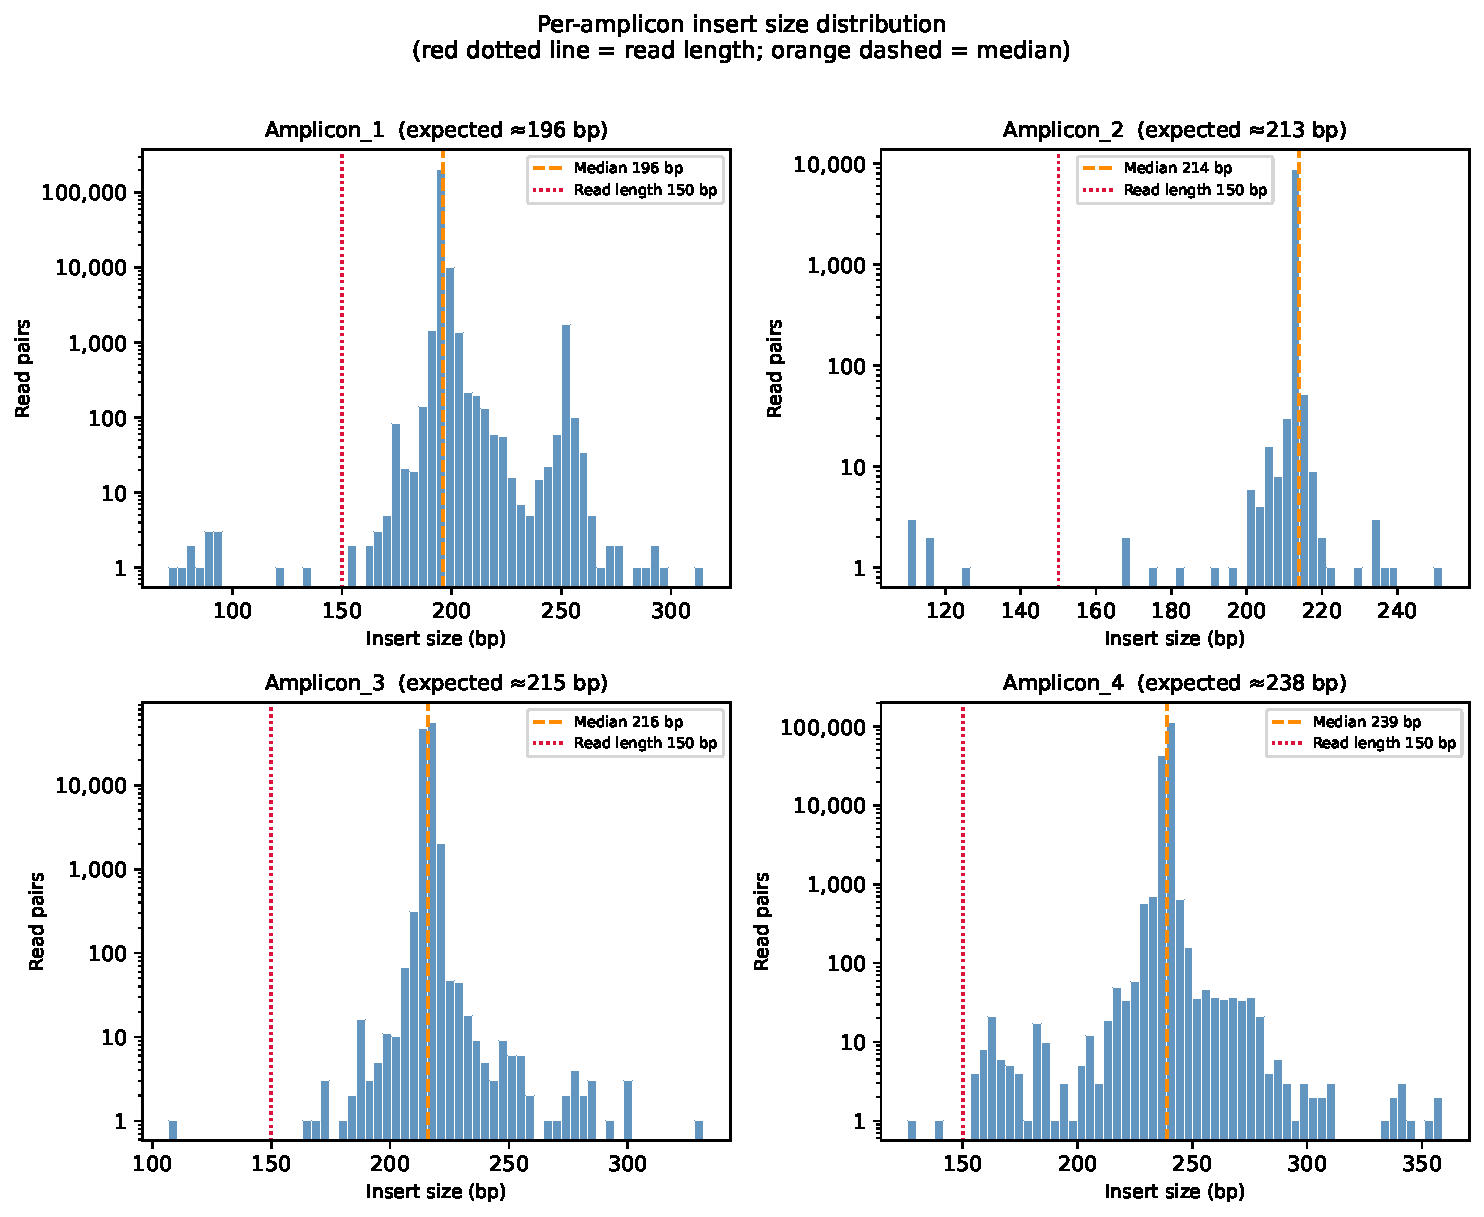
\includegraphics[width=\textwidth]{figures/insert_size_plot.pdf}
  \caption{Per-amplicon insert size distributions derived from the TLEN field
    of properly paired, mapped reads (\texttt{samtools view -f 2 -F 2308}).
    The y-axis is on a log scale to reveal low-frequency secondary peaks
    (e.g.\ primer-dimers, off-target products) that would be invisible on a
    linear scale given the dominant sharp peak of on-target amplicon fragments.
    Orange dashed line: median insert size for that amplicon.
    Red dotted line: read length (150\,bp) — amplicons with a distribution
    peak below this line generate read-through into the adaptor sequence.
    All four amplicons peak well above 150\,bp, consistent with the low
    read-through rates in Table~\ref{tab:per-amplicon-readthrough}.}
  \label{fig:insert-size}
\end{figure}

\subsubsection{Summary: read constitution}

Combining the findings above, each read has the following structure:

\begin{center}
\texttt{[Primer ($\sim$21--30\,bp)] $\rightarrow$ [Amplified region (135--187\,bp insert)] $\rightarrow$ [Adp\textsubscript{RC} (3' end, $\sim$6--11\% of reads only)]}
\end{center}

Primer sequences were confirmed at the expected 5' position in 95.9\% of read pairs
(Section~\ref{sec:primer-verification}).
The amplified region spans 135--187\,bp of insert sequence (Table~\ref{tab:amplicon-lengths}),
giving total amplicon lengths of 195--237\,bp --- all longer than the 150\,bp read length,
so R1 and R2 overlap in the centre of the amplicon rather than reading through into the
opposite adaptor.
Adaptor sequence at the 3' end was observed in $\sim$6\% of R1 reads and $\sim$11\% of R2
reads (Section~\ref{sec:adaptor-verification}), originating from a minority of shorter
fragments (degraded DNA, primer-dimers) where the read length exceeds the insert size.
This confirms the expected amplicon library structure illustrated in
Figure~\ref{fig:read-structure}.

% ============================================================
\section{Gene Region Mapping}
\label{sec:gene-region}
% ============================================================

\textbf{Question:} Which gene region did those reads map to?

Two complementary approaches were used to identify the targeted gene regions: first, the
primer sequences were aligned directly to hg19 using BLAST to establish the designed
amplicon coordinates; second, read coverage was computed from the BAM to confirm those
intervals with actual data and annotate overlapping genes.

\subsection{Primer Localisation by BLAST}
\label{sec:blast}

\paragraph{Methods.}
The eight primer sequences (four forward, four reverse; from \texttt{pipeline/config.yaml})
are written to a FASTA file by the Snakemake rule \texttt{blast\_primers}:

\begin{lstlisting}
>amplicon1_fwd   TTGCCAGTTAACGTCTTCCTTCTCTCTCTG
>amplicon1_rev   GAGAAAAGGTGGGCCTGAGGTTCAGAGCCA
>amplicon2_fwd   CCCTTGTCTCTGTGTTCTTGTCCCCCCCA
>amplicon2_rev   CCCCACCAGACCATGAGAGGCCCTGCGGCC
>amplicon3_fwd   TGATCTGTCCCTCACAGCAGGGTCTTCTCT
>amplicon3_rev   TGACCTAAAGCCACCTCCTTA
>amplicon4_fwd   CACACTGACGTGCCTCTCCCTCCCTCCA
>amplicon4_rev   CCGTATCTCCCTTCCCTGATTA
\end{lstlisting}

These are queried against a local BLAST nucleotide database built from the hg19 reference
FASTA (\texttt{hg19.fa.gz}, UCSC Genome Browser) using \texttt{makeblastdb}
.
The search uses parameters tuned for short sequences:

\begin{lstlisting}
blastn -query primers.fa -db hg19 \
    -task blastn-short \
    -word_size 7 \
    -evalue 1e-3 \
    -perc_identity 90 \
    -max_target_seqs 1 \
    -outfmt "6 qseqid sseqid pident length mismatch gapopen \
             qstart qend sstart send evalue bitscore sstrand"
\end{lstlisting}

\noindent Key parameter choices:
\begin{itemize}
  \item \texttt{-task blastn-short}: preset that lowers the word size and adjusts scoring
    for sequences $<$50\,bp. Standard \texttt{blastn} uses word size 11, which is too
    large to seed alignments reliably for 20--30\,bp primers.
  \item \texttt{-word\_size 7}: shorter seed increases sensitivity; acceptable here
    because we only query 8 sequences.
  \item \texttt{-evalue 1e-3}: permissive given the short query length; a 20\,bp perfect
    match against a 3\,Gbp genome has an E-value well below this cutoff.
  \item \texttt{-perc\_identity 90}: requires $\geq$90\% identity, filtering spurious
    low-identity hits while tolerating one or two mismatches.
  \item \texttt{-max\_target\_seqs 1}: reports only the top genomic hit per primer,
    giving the primary binding site.
\end{itemize}

Each amplicon's genomic span is defined as the interval from the forward primer hit start
to the reverse primer hit end on the same chromosome. The two one-time setup rules and
the search rule are:

\begin{lstlisting}
# One-time setup (download ~1 GB, build BLAST index):
bash pipeline/run.sh --cores 4 --until build_blast_db

# Run primer alignment:
bash pipeline/run.sh --cores 4 --until blast_primers
\end{lstlisting}

\paragraph{Results.}
% Auto-generated by pipeline/scripts/blast_primer_table.py via rule blast_primer_table.
% To regenerate: bash pipeline/run.sh --cores 4 --until blast_primer_table
% Auto-generated by pipeline/scripts/blast_primer_table.py — do not edit manually.
\begin{table}[H]
\centering
\begin{tabular}{lllllll}
\toprule
\textbf{Amplicon} & \textbf{Chr} & \textbf{Start (hg19)} & \textbf{End (hg19)} & \textbf{Length} & \textbf{Fwd id.} & \textbf{Rev id.} \\
\midrule
\texttt{Amplicon 1} & \texttt{chr7} & 55,242,379 & 55,242,574 & 195\,bp & 100\% & 100\% \\
\texttt{Amplicon 2} & \texttt{chr7} & 55,241,584 & 55,241,796 & 212\,bp & 100\% & 100\% \\
\texttt{Amplicon 3} & \texttt{chr7} & 55,259,375 & — & — & 100\% & no hit \\
\texttt{Amplicon 4} & \texttt{chr7} & 55,248,957 & 55,249,194 & 237\,bp & 100\% & 100\% \\
\bottomrule
\end{tabular}
\caption{Primer localisation by \texttt{blastn} against hg19 (\texttt{-task blastn-short}, \texttt{-perc\_identity 90}, \texttt{-evalue 1e-3}). Start and End define the amplicon span from forward primer start to reverse primer end. ``Fwd id.'' and ``Rev id.'' are the percent identity of the best BLAST hit; ``no hit'' indicates the primer fell below the E-value threshold.}
\label{tab:blast-primers}
\end{table}


All four forward primers align to \textbf{chr7} with 100\% identity, confirming that the
panel targets \textbf{EGFR} (Epidermal Growth Factor Receptor) on chromosome~7. The
primer coordinates span EGFR exons~18--21 (hg19 positions $\sim$55.24--55.26\,Mb),
the kinase domain hotspot region most commonly mutated in non-small-cell lung cancer.

The reverse primer for Amplicon~3 produced no hit at the $E < 10^{-3}$ threshold; this
primer is only 21\,bp (the shortest in the panel) and its best genomic match has
E~=~0.003, just above the cutoff. As shown in the off-target search
(Table~\ref{tab:blast-offtarget}), this hit is on chr7 with 100\% identity over all
21\,bp --- it is the correct EGFR binding site, merely filtered by the strict threshold.
Table~\ref{tab:blast-primers-relaxed} combines both searches to give complete coordinates
for all four amplicons.

% Auto-generated by pipeline/scripts/blast_primer_table_relaxed.py
% To regenerate: bash pipeline/run.sh --cores 4 --until blast_primer_table_relaxed
% Auto-generated by pipeline/scripts/blast_primer_table_relaxed.py
\begin{table}[H]
\centering
\begin{tabular}{lllllll}
\toprule
\textbf{Amplicon} & \textbf{Chr} & \textbf{Start (hg19)} & \textbf{End (hg19)} & \textbf{Length} & \textbf{Fwd id.} & \textbf{Rev id.} \\
\midrule
\texttt{Amplicon 1} & \texttt{chr7} & 55,242,379 & 55,242,574 & 195\,bp & 100\% & 100\% \\
\texttt{Amplicon 2} & \texttt{chr7} & 55,241,584 & 55,241,796 & 212\,bp & 100\% & 100\% \\
\texttt{Amplicon 3} & \texttt{chr7} & 55,259,375 & 55,259,589 & 214\,bp & 100\% & 100\%$^\dagger$ \\
\texttt{Amplicon 4} & \texttt{chr7} & 55,248,957 & 55,249,194 & 237\,bp & 100\% & 100\% \\
\bottomrule
\end{tabular}
\caption{Complete primer localisation combining the strict search (\texttt{-evalue~1e-3}) and the permissive off-target search. All four amplicons are resolved to chr7 (EGFR), including Amplicon~3 whose reverse primer was below the strict E-value threshold. $^\dagger$~Hit recovered from the permissive off-target search (\texttt{-evalue~1}; Table~\ref{tab:blast-offtarget}); E-value just exceeded the strict $10^{-3}$ cutoff.}
\label{tab:blast-primers-relaxed}
\end{table}


\paragraph{Off-target search (permissive BLAST).}
To check whether any primer could produce off-target amplification elsewhere in the genome,
the search was repeated with permissive parameters (rule \texttt{blast\_primers\_offtarget}):
\texttt{-max\_target\_seqs 10}, \texttt{-perc\_identity 70}, \texttt{-evalue 1}.
Table~\ref{tab:blast-offtarget} lists all secondary hits (primary EGFR hit per primer
excluded). All secondary hits have alignment lengths of 17--20\,bp and E-values
of 0.003--0.80 --- consistent with background noise rather than specific secondary
binding sites. Crucially, \textbf{none of these partial hits fall near chr4:77.6\,Mb},
ruling out off-target primer priming at the SHROOM3 locus observed in the coverage
analysis below.

% Auto-generated by pipeline/scripts/blast_offtarget_table.py via rule blast_offtarget_table.
% To regenerate: bash pipeline/run.sh --cores 4 --until blast_offtarget_table
% Auto-generated by pipeline/scripts/blast_offtarget_table.py
% via rule blast_offtarget_table
\begin{table}[H]
\centering
\small
\begin{tabular}{llrrrll}
\toprule
\textbf{Primer} & \textbf{Chr} & \textbf{Aln\,len\,(bp)} & \textbf{\%id} & \textbf{E-value} & \textbf{Strand} & \textbf{Type} \\
\midrule
\textbf{\texttt{amplicon1\_fwd}} & \textbf{chr7} & \textbf{30} & \textbf{100} & \textbf{3.35e-08} & \textbf{plus} & \textbf{\textit{on-target}} \\
 & chr19 & 18 & 100 & 0.49 & plus & \textit{off-target} \\
 & chrX & 18 & 100 & 0.49 & minus & \textit{off-target} \\
\addlinespace[4pt]
\textbf{\texttt{amplicon2\_fwd}} & \textbf{chr7} & \textbf{29} & \textbf{100} & \textbf{1.21e-07} & \textbf{plus} & \textbf{\textit{on-target}} \\
 & chr7 & 18 & 100 & 0.44 & plus & \textit{off-target} \\
 & chrY & 18 & 100 & 0.44 & plus & \textit{off-target} \\
 & chrY & 18 & 100 & 0.44 & minus & \textit{off-target} \\
\addlinespace[4pt]
\textbf{\texttt{amplicon3\_fwd}} & \textbf{chr7} & \textbf{30} & \textbf{100} & \textbf{3.35e-08} & \textbf{plus} & \textbf{\textit{on-target}} \\
 & chr7 & 20 & 100 & 0.03 & minus & \textit{off-target} \\
 & chr11 & 20 & 100 & 0.03 & minus & \textit{off-target} \\
 & chr3 & 20 & 100 & 0.03 & plus & \textit{off-target} \\
 & chr7 & 19 & 100 & 0.12 & minus & \textit{off-target} \\
 & chr4 & 19 & 100 & 0.12 & minus & \textit{off-target} \\
\addlinespace[4pt]
\textbf{\texttt{amplicon4\_fwd}} & \textbf{chr7} & \textbf{28} & \textbf{100} & \textbf{4.36e-07} & \textbf{plus} & \textbf{\textit{on-target}} \\
 & chr14 & 19 & 100 & 0.10 & minus & \textit{off-target} \\
 & chr14 & 18 & 100 & 0.40 & plus & \textit{off-target} \\
 & chr14 & 18 & 100 & 0.40 & plus & \textit{off-target} \\
 & chr22 & 18 & 100 & 0.40 & plus & \textit{off-target} \\
 & chr17 & 22 & 95 & 0.40 & plus & \textit{off-target} \\
 & chr17 & 18 & 100 & 0.40 & minus & \textit{off-target} \\
 & chr10 & 18 & 100 & 0.40 & plus & \textit{off-target} \\
 & chrX & 18 & 100 & 0.40 & plus & \textit{off-target} \\
 & chrX & 18 & 100 & 0.40 & minus & \textit{off-target} \\
 & chr6 & 18 & 100 & 0.40 & plus & \textit{off-target} \\
\addlinespace[4pt]
\textbf{\texttt{amplicon1\_rev}} & \textbf{chr7} & \textbf{30} & \textbf{100} & \textbf{3.35e-08} & \textbf{minus} & \textbf{\textit{on-target}} \\
 & chr15 & 20 & 100 & 0.03 & minus & \textit{off-target} \\
 & chr11 & 22 & 95 & 0.49 & plus & \textit{off-target} \\
\addlinespace[4pt]
\textbf{\texttt{amplicon2\_rev}} & \textbf{chr7} & \textbf{30} & \textbf{100} & \textbf{3.35e-08} & \textbf{minus} & \textbf{\textit{on-target}} \\
 & chr7 & 19 & 100 & 0.12 & minus & \textit{off-target} \\
 & chr18 & 18 & 100 & 0.49 & plus & \textit{off-target} \\
 & chr13 & 18 & 100 & 0.49 & plus & \textit{off-target} \\
\addlinespace[4pt]
\textbf{\texttt{amplicon3\_rev}} & \textbf{chr7} & \textbf{21} & \textbf{100} & \textbf{3.00e-03} & \textbf{minus} & \textbf{\textit{on-target (relaxed threshold)}} \\
 & chr1 & 19 & 100 & 0.04 & plus & \textit{off-target} \\
 & chr6 & 18 & 100 & 0.16 & minus & \textit{off-target} \\
 & chr13 & 17 & 100 & 0.64 & minus & \textit{off-target} \\
 & chrX & 17 & 100 & 0.64 & minus & \textit{off-target} \\
 & chr4 & 17 & 100 & 0.64 & minus & \textit{off-target} \\
\addlinespace[4pt]
\textbf{\texttt{amplicon4\_rev}} & \textbf{chr7} & \textbf{22} & \textbf{100} & \textbf{8.29e-04} & \textbf{minus} & \textbf{\textit{on-target}} \\
 & chr10 & 17 & 100 & 0.80 & plus & \textit{off-target} \\
 & chr6 & 17 & 100 & 0.80 & minus & \textit{off-target} \\
 & chr4 & 17 & 100 & 0.80 & minus & \textit{off-target} \\
\bottomrule
\end{tabular}
\caption{All hits from the permissive off-target BLAST search (\texttt{-perc\_identity~70}, \texttt{-evalue~1}, \texttt{-max\_target\_seqs~10}). \textbf{Bold} rows are the best hit per primer: \textbf{\textit{on-target}} primers were also found in the strict search (Table~\ref{tab:blast-primers}); \textbf{\textit{on-target (relaxed threshold)}} indicates the primer's best hit is the correct EGFR site but its E-value (0.003) just exceeded the strict cutoff of $10^{-3}$. Normal-weight rows are secondary \textit{off-target} hits sorted by E-value within each primer; all have alignment lengths of 17--21\,bp and E-values~$\geq 0.003$, consistent with background noise. No off-target hit falls near chr4:77.6\,Mb (SHROOM3 locus).}
\label{tab:blast-offtarget}
\end{table}


\paragraph{Amplicon structure and read coverage.}
Each amplicon sequenced on the MiSeq consists of three contiguous parts:
the \textcolor{green!50!black}{\textbf{forward primer}}, the \textbf{biological
insert} (the region of interest carrying any variants), and the
\textcolor{orange!60!black}{\textbf{reverse primer}}.
The total amplicon length reported by BLAST is therefore
$l_\mathrm{amp} = l_\mathrm{fwd} + l_\mathrm{insert} + l_\mathrm{rev}$
(Figure~\ref{fig:amplicon-structure}a).

In paired-end sequencing, R1 reads inward from the forward primer and R2 reads
inward from the reverse primer (Figure~\ref{fig:amplicon-structure}b).
Because all four amplicons are \emph{longer} than the read length
($l_\mathrm{amp} = 195$--$237$\,bp $> r = 150$\,bp), each read terminates
inside the amplicon before reaching the far adapter --- explaining the near-zero
read-through rates ($<$5\%) observed in Section~\ref{sec:read-constitution}.
At the same time, because all amplicons are shorter than twice the read length
($l_\mathrm{amp} < 2r = 300$\,bp), R1 and R2 do meet in the centre,
overlapping by $2r - l_\mathrm{amp}$ bases (Table~\ref{tab:amplicon-lengths}).

\begin{figure}[H]
\centering
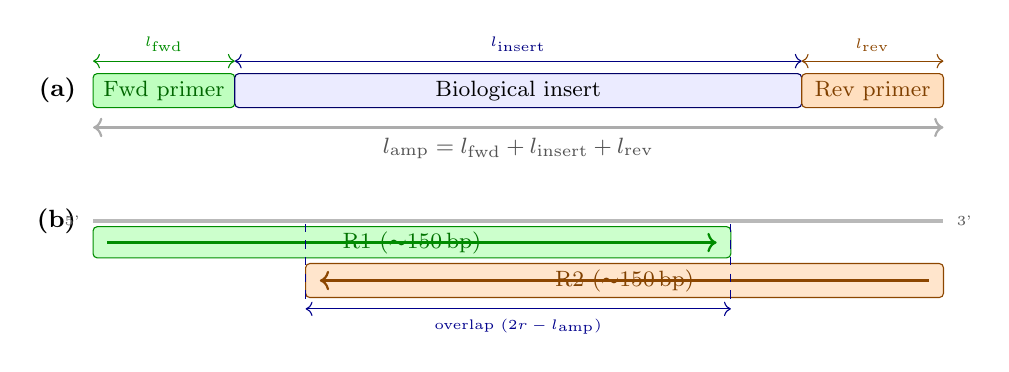
\begin{tikzpicture}[x=0.9cm, y=0.72cm, font=\small]

  % ────────────────────────────────────────────────────────────────────
  % (a)  Amplicon = Fwd primer + Biological insert + Rev primer
  % ────────────────────────────────────────────────────────────────────
  \node[left, font=\small\bfseries] at (-0.1, 0.3) {(a)};

  % Fwd primer block (green, ~2/12 of total)
  \filldraw[fill=green!25, draw=green!55!black, rounded corners=1.5pt]
    (0,0) rectangle (2,0.6);
  \node[font=\footnotesize, green!40!black] at (1,0.3) {Fwd primer};

  % Biological insert block (blue-gray)
  \filldraw[fill=blue!8, draw=blue!40!black, rounded corners=1.5pt]
    (2,0) rectangle (10,0.6);
  \node[font=\footnotesize] at (6,0.3) {Biological insert};

  % Rev primer block (orange, ~2/12 of total)
  \filldraw[fill=orange!25, draw=orange!55!black, rounded corners=1.5pt]
    (10,0) rectangle (12,0.6);
  \node[font=\footnotesize, orange!50!black] at (11,0.3) {Rev primer};

  % Length annotation braces (above)
  \draw[<->, thin, green!55!black]  (0,0.82)  -- (2,0.82)
    node[midway, above, font=\tiny]  {$l_\mathrm{fwd}$};
  \draw[<->, thin, blue!50!black]   (2,0.82)  -- (10,0.82)
    node[midway, above, font=\tiny]  {$l_\mathrm{insert}$};
  \draw[<->, thin, orange!55!black] (10,0.82) -- (12,0.82)
    node[midway, above, font=\tiny]  {$l_\mathrm{rev}$};

  % Amplicon total span (below)
  \draw[<->, thick, gray!65] (0,-0.35) -- (12,-0.35)
    node[midway, below, font=\footnotesize, gray!65!black] {$l_\mathrm{amp} = l_\mathrm{fwd} + l_\mathrm{insert} + l_\mathrm{rev}$};

  % ────────────────────────────────────────────────────────────────────
  % (b)  R1 / R2 read directions and overlap (schematic, ~150 bp reads)
  %      Using proportions: total = 12 u, read length = 9 u → overlap = 6 u
  % ────────────────────────────────────────────────────────────────────
  \node[left, font=\small\bfseries] at (-0.1,-2.0) {(b)};

  % Amplicon backbone
  \draw[very thick, gray!55] (0,-2.0) -- (12,-2.0);
  \node[left,  font=\tiny, gray!70!black] at (-0.05,-2.0) {5'};
  \node[right, font=\tiny, gray!70!black] at (12.05,-2.0) {3'};

  % ── R1: starts at fwd primer, reads rightward, ~150 bp ──
  \filldraw[fill=green!20, draw=green!55!black, rounded corners=1.5pt]
    (0,-2.65) rectangle (9,-2.1);
  \node[font=\footnotesize, green!45!black] at (4.5,-2.38) {R1 ($\sim$150\,bp)};
  \draw[->, thick, green!55!black] (0.2,-2.38) -- (8.8,-2.38);

  % ── R2: starts at rev primer, reads leftward, ~150 bp ──
  \filldraw[fill=orange!20, draw=orange!55!black, rounded corners=1.5pt]
    (3,-3.35) rectangle (12,-2.75);
  \node[font=\footnotesize, orange!50!black] at (7.5,-3.05) {R2 ($\sim$150\,bp)};
  \draw[<-, thick, orange!55!black] (3.2,-3.05) -- (11.8,-3.05);

  % ── Overlap region ──
  \draw[dashed, blue!55!black, thin] (3,-2.05)  -- (3,-3.45);
  \draw[dashed, blue!55!black, thin] (9,-2.05)  -- (9,-3.45);
  \draw[<->, blue!55!black] (3,-3.55) -- (9,-3.55)
    node[midway, below, font=\tiny, blue!55!black]
      {overlap ($2r - l_\mathrm{amp}$)};

\end{tikzpicture}
\caption{(a)~An amplicon consists of the forward primer, the biological insert, and the
reverse primer. The total amplicon length is $l_\mathrm{amp} = l_\mathrm{fwd} +
l_\mathrm{insert} + l_\mathrm{rev}$; BLAST primer localisation reports
$l_\mathrm{amp}$ directly as the span from forward primer start to reverse primer end.
(b)~R1 reads inward from the forward primer; R2 reads inward from the reverse primer.
When $l_\mathrm{amp} < 2r$ (where $r \approx 150$\,bp is the read length), the two reads
overlap in the centre by $2r - l_\mathrm{amp}$ bases. Schematic proportions; not to
exact scale.}
\label{fig:amplicon-structure}
\end{figure}


% Auto-generated by pipeline/scripts/amplicon_length_table.py via rule amplicon_length_table.
% To regenerate: bash pipeline/run.sh --cores 4 --until amplicon_length_table
% Auto-generated by pipeline/scripts/amplicon_length_table.py
% via rule amplicon_length_table
\begin{table}[H]
\centering
\begin{tabular}{lrrrrr}
\toprule
\textbf{Amplicon} & \textbf{Amp. length} & \textbf{Fwd primer} & \textbf{Insert} & \textbf{Rev primer} & \textbf{R1/R2 overlap} \\
\midrule
Amplicon~1 & 195\,bp & 30\,bp & 135\,bp & 30\,bp & 105\,bp \\
Amplicon~2 & 212\,bp & 29\,bp & 153\,bp & 30\,bp & 88\,bp \\
Amplicon~3 & 214\,bp & 30\,bp & 163\,bp & 21\,bp & 86\,bp \\
Amplicon~4 & 237\,bp & 28\,bp & 187\,bp & 22\,bp & 63\,bp \\
\bottomrule
\end{tabular}
\caption{Amplicon composition derived from BLAST primer coordinates (Table~\ref{tab:blast-primers-relaxed}) and primer sequences (Table~\ref{tab:primers}). Insert length $= l_\mathrm{amp} - l_\mathrm{fwd} - l_\mathrm{rev}$. R1/R2 overlap $= 2r - l_\mathrm{amp}$ where $r = 150$\,bp; positive values indicate the two reads overlap in the centre of the amplicon (see Figure~\ref{fig:amplicon-structure}).}
\label{tab:amplicon-lengths}
\end{table}


\paragraph{Gene annotation of targeted amplicons.}
To confirm which genes the four amplicons target, the BLAST-derived amplicon coordinates
(Table~\ref{tab:blast-primers-relaxed}) were intersected with the hg19 RefFlat gene
annotation using \texttt{bedtools intersect -wo}.
Table~\ref{tab:blast-gene-intersect} shows that all four amplicons map entirely within the
\emph{EGFR} gene (100\% overlap), confirming that the panel is a targeted EGFR sequencing
assay.
Amplicon~4 additionally overlaps \emph{EGFR-AS1}, a long non-coding antisense RNA whose
locus is embedded within the EGFR gene body on the opposite strand; this is an expected
annotation artefact rather than an off-target design.

\paragraph{Background: EGFR and EGFR-AS1.}
\emph{EGFR} (Epidermal Growth Factor Receptor; chr7p11.2) encodes a transmembrane receptor
tyrosine kinase of the ErbB family. Upon ligand binding, EGFR homo- or heterodimerises
and activates downstream proliferation and survival pathways (RAS/MAPK, PI3K/AKT)~\cite{yarden2001}.
Somatic activating mutations in EGFR --- most commonly in-frame deletions in exon~19 and the
L858R point mutation in exon~21 --- are driver events in non-small-cell lung cancer (NSCLC)
and confer sensitivity to EGFR tyrosine kinase inhibitors such as gefitinib and
erlotinib~\cite{lynch2004}.
Each amplicon covers exactly one exon of the kinase-domain hotspot: Amplicon~2 covers
exon~18 (G719 mutations), Amplicon~1 covers exon~19 (common in-frame deletions),
Amplicon~4 covers exon~20 (insertion hotspot), and Amplicon~3 covers exon~21
(L858R substitution).
Together the four amplicons span the full exon~18--21 mutational hotspot,
consistent with a clinical EGFR variant-detection assay (Figure~\ref{fig:egfr-exon}).

\emph{EGFR-AS1} (EGFR Antisense RNA~1) is a long non-coding RNA (lncRNA) transcribed from
the antisense strand of the EGFR locus and annotated as a separate gene entry in RefSeq.
Because it occupies the same genomic interval as EGFR on the opposite strand, any amplicon
spanning that region will intersect both entries in a strand-agnostic BED intersection ---
hence the dual annotation for Amplicon~4.
EGFR-AS1 has been reported to modulate EGFR mRNA levels in \emph{cis}, but its functional
role remains an active area of research; it is not a target of this sequencing panel.

% Auto-generated by pipeline/scripts/blast_gene_intersect_table.py via rule blast_gene_intersect.
% To regenerate: bash pipeline/run.sh --cores 4 --until blast_gene_intersect
% Auto-generated by pipeline/scripts/blast_gene_intersect_table.py
% via rule blast_gene_intersect
\begin{table}[H]
\centering
\begin{tabular}{llrrr}
\toprule
\textbf{Amplicon} & \textbf{Gene} & \textbf{Amp.\ len (bp)} & \textbf{Overlap (bp)} & \textbf{Overlap (\%)} \\
\midrule
Amplicon~1 & EGFR & 196 & 196 & 100.0 \\
\addlinespace[3pt]
Amplicon~2 & EGFR & 213 & 213 & 100.0 \\
\addlinespace[3pt]
Amplicon~3 & EGFR & 215 & 215 & 100.0 \\
\addlinespace[3pt]
Amplicon~4 & EGFR & 238 & 238 & 100.0 \\
 & EGFR-AS1 & 238 & 238 & 100.0 \\
\bottomrule
\end{tabular}
\caption{Gene overlaps for the four BLAST-defined amplicon intervals (Table~\ref{tab:blast-primers-relaxed}), computed with \texttt{bedtools intersect -wo} against the hg19 RefFlat gene annotation. Overlap is reported in base pairs and as a percentage of the amplicon length.}
\label{tab:blast-gene-intersect}
\end{table}


Table~\ref{tab:egfr-exons} lists the four targeted exons with their exact hg19 coordinates
and the associated somatic mutations relevant to NSCLC diagnosis and treatment.
Exons~19 and~21 together account for approximately 85\% of all oncogenic EGFR
alterations; exon~18 G719X and exon~20 insertions make up most of the remainder.
The panel therefore covers the full spectrum of clinically actionable EGFR variants
screened in routine oncology practice.

% Auto-generated by pipeline/scripts/egfr_exon_table.py via rule egfr_exon_table.
% To regenerate: bash pipeline/run.sh --cores 4 --until egfr_exon_table
% then copy pipeline/results/tables/egfr_exon_table.tex to report/tables/
% Auto-generated by pipeline/scripts/egfr_exon_table.py
% via rule egfr_exon_table
\begin{table}[H]
\centering
\small
\resizebox{\textwidth}{!}{%
\begin{tabular}{cclrrp{7cm}}
\toprule
\textbf{Exon} & \textbf{Amplicon} & \textbf{Start (hg19)} & \textbf{End (hg19)} & \textbf{Len (bp)} & \textbf{Known somatic mutations} \\
\midrule
18 & Amplicon~2 & 55{,}241{,}613 & 55{,}241{,}736 & 123 & G719X point mutations; uncommon ($\sim$3\% of EGFR mutations), sensitive to afatinib and osimertinib \\
\addlinespace[3pt]
19 & Amplicon~1 & 55{,}242{,}414 & 55{,}242{,}513 & 99 & In-frame deletions (e.g.\ E746\_A750del); most common EGFR alteration ($\sim$45\%), strongly sensitive to EGFR TKIs \\
\addlinespace[3pt]
20 & Amplicon~4 & 55{,}248{,}985 & 55{,}249{,}171 & 186 & In-frame insertions; generally confer resistance to first/second-generation TKIs; targeted by amivantamab and mobocertinib \\
\addlinespace[3pt]
21 & Amplicon~3 & 55{,}259{,}411 & 55{,}259{,}567 & 156 & L858R point mutation (c.2573T$>$G); second most common EGFR alteration ($\sim$40\%), sensitive to EGFR TKIs \\
\bottomrule
\end{tabular}%
}% end resizebox
\caption{EGFR kinase-domain exons targeted by the amplicon panel (NM\_005228, hg19, plus strand). Coordinates are 0-based half-open (BED convention), derived from the UCSC hg19 refFlat table. Exons~18--21 together account for $\gtrsim$85\% of all oncogenic EGFR mutations and are the primary predictive biomarkers for tyrosine kinase inhibitor (TKI) therapy in non-small-cell lung cancer (NSCLC)~\cite{lynch2004}.}
\label{tab:egfr-exons}
\end{table}


\paragraph{Amplicon coverage of target exons.}
Each amplicon fully contains its target exon: the primers are placed in the flanking
intronic sequence on either side, so the sequenced region spans a short intronic flank,
the complete exon, and another short intronic flank.
Table~\ref{tab:amplicon-exon-overlap} gives the exact amplicon and exon coordinates
alongside the left and right intronic flanks for each amplicon.

% Auto-generated by pipeline/scripts/amplicon_exon_overlap_table.py
% via rule amplicon_exon_overlap_table.
% To regenerate: bash pipeline/run.sh --cores 4 --until amplicon_exon_overlap_table
% Auto-generated by pipeline/scripts/amplicon_exon_overlap_table.py
% via rule amplicon_exon_overlap_table
\begin{table}[H]
\centering
\small
\begin{tabular}{clrrrrrr}
\toprule
\textbf{Exon} & \textbf{Amplicon} & \textbf{Amp.~start} & \textbf{Amp.~end} & \textbf{Amp.~len} & \textbf{Exon start} & \textbf{Exon end} & \textbf{Exon len} \\
 & & & & \textbf{(bp)} & & & \textbf{(bp)} \\
\midrule
18 & Amplicon~2 & 55{,}241{,}583 & 55{,}241{,}796 & 213 & 55{,}241{,}613 & 55{,}241{,}736 & 123 \\
19 & Amplicon~1 & 55{,}242{,}378 & 55{,}242{,}574 & 196 & 55{,}242{,}414 & 55{,}242{,}513 & 99 \\
20 & Amplicon~4 & 55{,}248{,}956 & 55{,}249{,}194 & 238 & 55{,}248{,}985 & 55{,}249{,}171 & 186 \\
21 & Amplicon~3 & 55{,}259{,}374 & 55{,}259{,}589 & 215 & 55{,}259{,}411 & 55{,}259{,}567 & 156 \\
\bottomrule
\end{tabular}
\caption{Amplicon spans relative to their target EGFR exon (NM\_005228, hg19, plus strand, 0-based half-open coordinates). Each amplicon fully contains its target exon; the primers are placed in the flanking intronic sequence on either side. Left intronic flank = exon~start $-$ amplicon~start; right intronic flank = amplicon~end $-$ exon~end.}
\label{tab:amplicon-exon-overlap}
\end{table}


% Auto-generated by pipeline/scripts/egfr_exon_figure.py via rule egfr_exon_figure.
% To regenerate: bash pipeline/run.sh --cores 4 --until egfr_exon_figure
% then copy pipeline/results/figures/egfr_exon_figure.pdf to report/figures/
\begin{figure}[H]
\centering
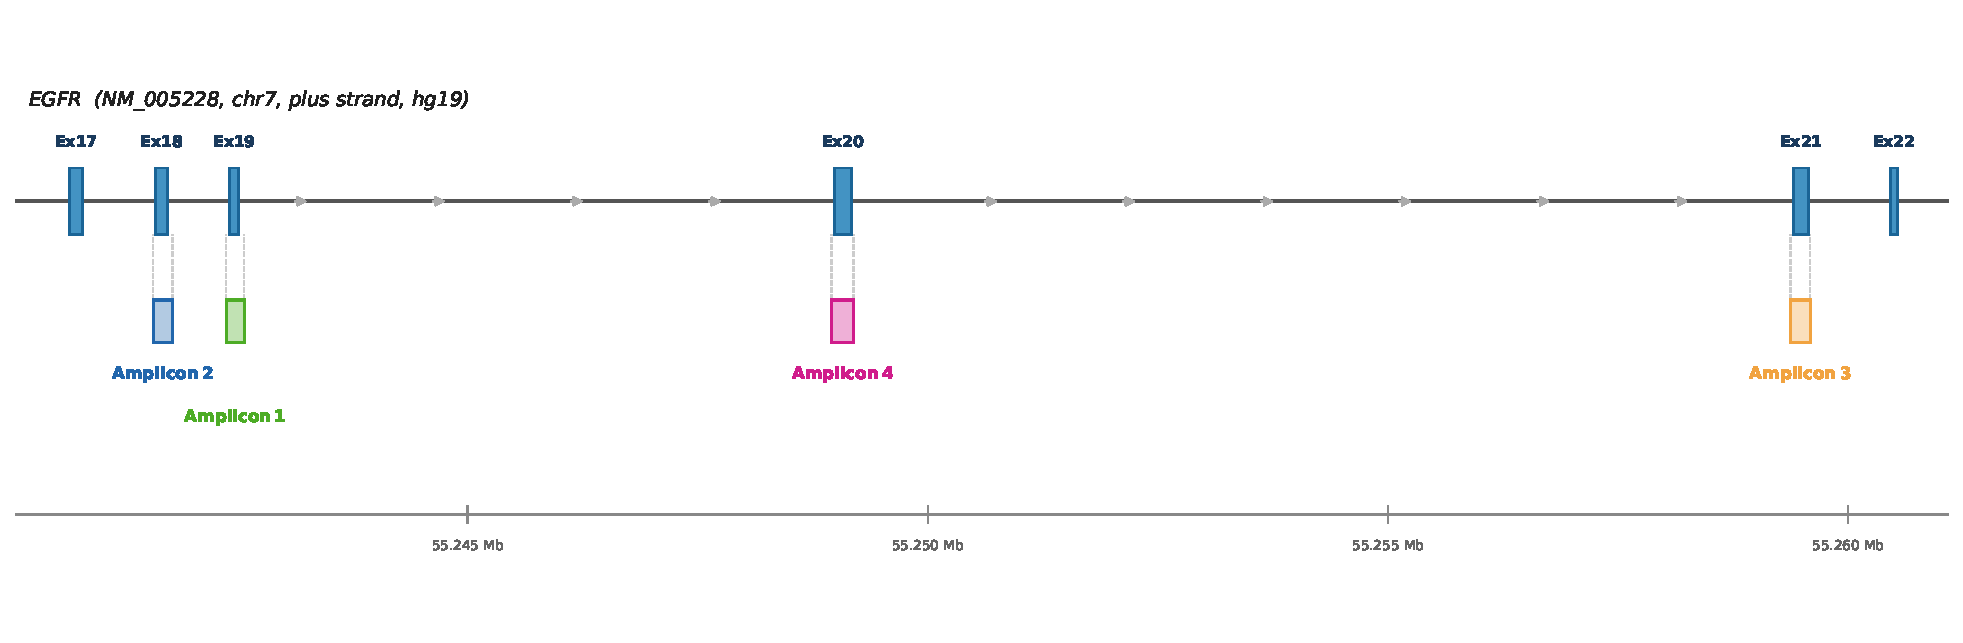
\includegraphics[width=\textwidth]{figures/egfr_exon_figure.pdf}
\caption{Exon structure of EGFR (NM\_005228, hg19, chr7 plus strand) in the region
targeted by the amplicon panel. Blue boxes indicate exons; exon numbers follow the
canonical transcript order (5$'$ to 3$'$, left to right). The four amplicons (coloured
bars) were localised by BLAST primer alignment (Table~\ref{tab:blast-primers-relaxed}).
Each amplicon spans exactly one exon: Amplicon~2 covers exon~18 (G719 mutation site),
Amplicon~1 covers exon~19 (the most common site of in-frame deletions in
NSCLC~\cite{lynch2004}), Amplicon~4 covers exon~20 (insertion hotspot), and
Amplicon~3 covers exon~21 (L858R substitution site~\cite{lynch2004}).
Together the four amplicons span the full kinase-domain mutational hotspot (exons~18--21).
Genomic coordinates are hg19 (GRCh37).}
\label{fig:egfr-exon}
\end{figure}


\subsection{Coverage-Based Region Identification}

\paragraph{Methods.}
Covered genomic intervals were identified from \texttt{aln.bam} using a three-step
\texttt{bedtools} (v2.31.1)~\cite{quinlan2010} pipeline (rule \texttt{task2\_gene\_region}):
per-base depth was computed with \texttt{genomecov -bg}, positions below 10,000$\times$
were filtered to exclude scattered off-target reads, adjacent high-coverage positions were
merged into amplicon-level intervals with \texttt{bedtools merge}, and each interval was
annotated against hg19 RefFlat gene models\footnote{%
  RefFlat is a flat-file table format maintained by the UCSC Genome Browser that
  describes known RefSeq transcript models. Each row encodes one transcript: gene symbol,
  accession, chromosome, strand, transcription start/end, CDS boundaries, exon count, and
  exon coordinates. Derived from the NCBI RefSeq curated gene set, it is widely used as a
  lightweight, single-file alternative to GTF/GFF annotation for interval-based operations
  such as genomic-region annotation.}
stored in \texttt{pipeline/\allowbreak resources/\allowbreak hg19\_genes.bed}.
The 10,000$\times$ depth threshold separates amplicon coverage (100,000--440,000$\times$)
from scattered off-target reads (1--500$\times$).

\paragraph{Results.}

The bedtools pipeline identified five high-coverage amplicon intervals at a minimum depth
of 10,000$\times$, annotated against the hg19 RefFlat gene models:

% Auto-generated by pipeline/scripts/gene_region_table_bedtools.py via rule task2_gene_region.
% To regenerate: bash pipeline/run.sh --cores 4 --until task2_gene_region
% then run: bash report/copy_generated_files.sh
% Auto-generated by pipeline/scripts/gene_region_table_bedtools.py — do not edit manually.
\begin{table}[H]
\centering
\begin{tabular}{llll}
\toprule
\textbf{Chr} & \textbf{Start (hg19)} & \textbf{End (hg19)} & \textbf{Gene(s)} \\
\midrule
\texttt{chr4} & 77,620,760 & 77,620,951 & \textit{SHROOM3} \\
\texttt{chr7} & 55,241,646 & 55,241,734 & \textit{EGFR} \\
\texttt{chr7} & 55,242,378 & 55,242,574 & \textit{EGFR} \\
\texttt{chr7} & 55,248,956 & 55,249,194 & \textit{EGFR, EGFR-AS1} \\
\texttt{chr7} & 55,259,374 & 55,259,589 & \textit{EGFR} \\
\bottomrule
\end{tabular}
\caption{Amplicon regions covered by the BAM (\texttt{bedtools genomecov} $\to$ \texttt{bedtools merge}), annotated against hg19 RefFlat gene models (\texttt{bedtools intersect}). Start and End are the exact covered-base boundaries as reported by \texttt{bedtools merge}.}
\label{tab:gene-regions}
\end{table}


\begin{figure}[H]
\centering
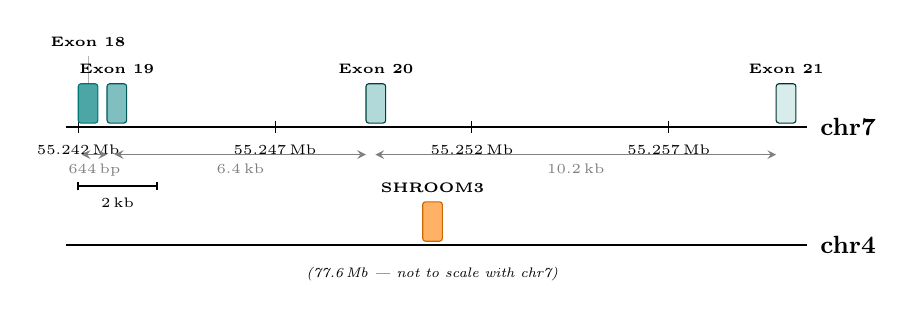
\begin{tikzpicture}[x=0.5cm, y=1cm, font=\footnotesize]

  % ---- chr7 axis ----
  % Coordinates in kb, offset from 55,241,646 (= 0 kb)
  % Amp1 (ex18): 0.000–0.088 kb   Amp2 (ex19): 0.732–0.928 kb
  % Amp3 (ex20): 7.310–7.548 kb   Amp4 (ex21): 17.728–17.943 kb

  % chromosome backbone
  \draw[thick] (-0.3, 0) -- (18.5, 0);
  \node[right, font=\small\bfseries] at (18.6, 0) {chr7};

  % kb tick marks every 5 kb with Mb labels
  \foreach \kb/\lbl in {0/55.242, 5/55.247, 10/55.252, 15/55.257} {
    \draw (\kb, 0.08) -- (\kb, -0.08);
    \node[below, font=\tiny] at (\kb, -0.1) {\lbl\,Mb};
  }

  % amplicons — drawn with min display width 0.5 kb; actual widths are 88–238 bp
  % colours: teal shades for EGFR amplicons
  \filldraw[fill=teal!70, draw=teal!90!black, rounded corners=1pt]
    (0.000, 0.05) rectangle (0.50, 0.55);
  \filldraw[fill=teal!50, draw=teal!70!black, rounded corners=1pt]
    (0.732, 0.05) rectangle (1.23, 0.55);
  \filldraw[fill=teal!30, draw=teal!50!black, rounded corners=1pt]
    (7.310, 0.05) rectangle (7.81, 0.55);
  \filldraw[fill=teal!15, draw=teal!40!black, rounded corners=1pt]
    (17.728, 0.05) rectangle (18.23, 0.55);

  % amplicon labels above — Exon 18 raised to avoid overlap with Exon 19
  \node[above, font=\tiny\bfseries] at (0.25,  0.90) {Exon 18};
  \draw[gray!60, thin] (0.25, 0.56) -- (0.25, 0.90);
  \node[above, font=\tiny\bfseries] at (0.98,  0.55) {Exon 19};
  \node[above, font=\tiny\bfseries] at (7.56,  0.55) {Exon 20};
  \node[above, font=\tiny\bfseries] at (17.98, 0.55) {Exon 21};

  % ---- gap annotations below axis ----
  % Gap A1→A2: 0.088 → 0.732 = 644 bp
  \draw[<->, >=stealth, gray] (0.088, -0.35) -- (0.732, -0.35);
  \node[below, gray] at (0.41, -0.35) {\tiny 644\,bp};

  % Gap A2→A3: 0.928 → 7.310 = 6,382 bp
  \draw[<->, >=stealth, gray] (0.928, -0.35) -- (7.310, -0.35);
  \node[below, gray] at (4.12, -0.35) {\tiny 6.4\,kb};

  % Gap A3→A4: 7.548 → 17.728 = 10,180 bp
  \draw[<->, >=stealth, gray] (7.548, -0.35) -- (17.728, -0.35);
  \node[below, gray] at (12.64, -0.35) {\tiny 10.2\,kb};

  % ---- scale bar ----
  \draw[thick] (0, -0.75) -- (2, -0.75);
  \draw[thick] (0, -0.70) -- (0, -0.80);
  \draw[thick] (2, -0.70) -- (2, -0.80);
  \node[below] at (1, -0.78) {\tiny 2\,kb};

  % ---- chr4 (separate chromosome, schematic only) ----
  \draw[thick] (-0.3, -1.5) -- (18.5, -1.5);
  \node[right, font=\small\bfseries] at (18.6, -1.5) {chr4};
  \node[below, font=\tiny] at (9.0, -1.65) {\textit{(77.6\,Mb — not to scale with chr7)}};

  % SHROOM3 — positioned at centre for schematic representation
  \filldraw[fill=orange!60, draw=orange!80!black, rounded corners=1pt]
    (8.75, -1.45) rectangle (9.25, -0.95);
  \node[above, font=\tiny\bfseries] at (9.0, -0.95) {SHROOM3};
  \node[below, font=\tiny] at (9.0, -1.65) {};

\end{tikzpicture}
\caption{Relative genomic positions of the five covered intervals on chr7 and chr4 (hg19).
  The chr7 axis is drawn to scale: the four EGFR amplicons span $\sim$18\,kb in total,
  with a 644\,bp gap between exons~18 and~19, a 6.4\,kb gap to exon~20, and a 10.2\,kb gap
  to exon~21. Amplicon widths are exaggerated for visibility (actual widths 88--238\,bp).
  The chr4 SHROOM3 interval (77.6\,Mb) is shown schematically and is not to scale
  relative to chr7.}
\label{fig:amplicon-positions}
\end{figure}


The coverage confirms the BLAST findings: all four amplicons pile up on \textbf{EGFR} on
chromosome~7 (positions 55.2--55.3\,Mb, hg19), spanning the kinase domain hotspot region
encoding exons~18--21. EGFR mutations here are the most clinically actionable alterations
in non-small-cell lung cancer (NSCLC), guiding treatment with tyrosine kinase inhibitors
(TKIs) such as gefitinib, erlotinib, and osimertinib. One chr7 interval also overlaps
\textbf{EGFR-AS1}, an antisense lncRNA transcribed from the same locus.

The table contains five intervals despite the panel having only four primer pairs.
As confirmed by the BLAST primer coordinates (Table~\ref{tab:blast-primers}), Amplicons~1
and~2 are two separate amplicons on chr7 with a 644\,bp intronic gap that 150\,bp reads
cannot bridge, producing two distinct coverage intervals rather than one.

A fifth interval maps to \textbf{SHROOM3} on chromosome~4 (77.6\,Mb, hg19). As shown by
the BLAST analysis above, none of the panel's primers bind near chr4:77.6\,Mb even at
highly permissive thresholds, so this is not a designed amplicon target. Three alternative
mechanisms could explain the $\sim$30,000 reads mapping there:
\begin{itemize}
  \item \textbf{Read misalignment due to sequence similarity.} The SHROOM3 genomic
    region may share a repetitive element (e.g.\ SINE or LINE transposon) with the EGFR
    amplicons, causing the aligner to place a subset of EGFR-derived reads there.
    The reads being concentrated in a narrow 191\,bp window is consistent with a shared
    repeat locus.
  \item \textbf{Index hopping.} A known Illumina phenomenon in which a small fraction
    of reads are mis-assigned to the wrong sample barcode during cluster generation.
    If a co-sequenced library targets chr4:77.6\,Mb, those reads could appear in this
    sample at low abundance.
  \item \textbf{Chimeric PCR artefacts.} Partially complementary strands can join
    during PCR and produce chimeric products that map to SHROOM3 irrespective of primer
    design.
\end{itemize}
Distinguishing between these mechanisms would require further investigation.

The \texttt{Mapped reads} column reports total per-chromosome read counts from
\texttt{samtools idxstats}; for chromosomes with multiple amplicons (chr7), this count
is shared across all rows. Per-amplicon depth is quantified in Section~\ref{sec:coverage}.

% ============================================================
\section{Mapping Rate and Unmapped Reads}
\label{sec:mapping-rate}
% ============================================================

\textbf{Question:} What is the percentage of reads that were mapped to the human genome?
Can you give some comments on the unmapped reads?

\subsection{Methods}

Mapping statistics were obtained by running \texttt{samtools flagstat} on the
pre-aligned BAM file:

\begin{lstlisting}[language=bash]
samtools flagstat aln.bam > flagstat.txt
\end{lstlisting}

Unmapped reads were extracted into a compressed FASTQ for downstream
characterisation:

\begin{lstlisting}[language=bash]
samtools view -f 4 -b aln.bam | samtools fastq - | gzip > unmapped.fastq.gz
\end{lstlisting}

Both steps are encoded as Snakemake rules (\texttt{task3\_flagstat} and
\texttt{task3\_unmapped\_reads}) and the summary table is generated by
\texttt{task3\_flagstat\_table}. To reproduce:

\begin{lstlisting}[language=bash]
bash pipeline/run.sh --cores 4 --until task3_flagstat_table task3_unmapped_reads
\end{lstlisting}

\subsection{Results}

Of 1{,}150{,}004 total reads, 1{,}052{,}983 (91.56\%) mapped to the human reference
genome (hg19), leaving 97{,}021 reads (8.44\%) unmapped (Table~\ref{tab:flagstat}).
The mapping rate is consistent with the on-target rate of 94.3\% reported in
Section~\ref{sec:coverage-uniformity}: at the aggregate level, the great majority of
sequenced fragments originate from the four EGFR amplicons. However, these overall
figures mask a pronounced per-amplicon imbalance: Amplicon~2 carries only 1.9\% of
assigned read pairs and has an 89\% unmapped rate, discussed in detail in
Section~\ref{sec:coverage}.
No duplicate reads were detected, which is expected for a targeted amplicon
panel where PCR duplication cannot be distinguished from independent capture of
the same molecule.
Singletons (one mate unmapped) account for only 0.31\% of reads, and mates
mapping to a different chromosome are negligible (0.06\%), indicating clean and
concordant paired-end sequencing.

% Auto-generated by pipeline/scripts/flagstat_table.py
% via rule task3_flagstat_table.
% To regenerate: bash pipeline/run.sh --cores 4 --until task3_flagstat_table
% Auto-generated by pipeline/scripts/flagstat_table.py
% via rule task3_flagstat_table.
\begin{table}[H]
  \centering
  \begin{tabular}{lrr}
    \toprule
    \textbf{Metric} & \textbf{Reads} & \textbf{\%} \\
    \midrule
  Total reads & 1,150,004 & 100.00\% \\
  Mapped & 1,052,983 & 91.56\% \\
  Unmapped & 97,021 & 8.44\% \\
  Properly paired & 1,046,208 & 90.97\% \\
  Singletons & 3,583 & 0.31\% \\
  Mate on diff.\ chr ($\geq$MQ5) & 646 & 0.06\% \\
  Duplicates & 0 & 0.00\% \\
    \bottomrule
  \end{tabular}
  \caption{%
    Mapping statistics from \texttt{samtools flagstat}.
    Percentages are relative to the total number of reads.
    Duplicate marking was not performed (\textit{duplicates} = 0).
  }
  \label{tab:flagstat}
\end{table}



\subsubsection{Which amplicons do the unmapped reads target?}
To identify whether the unmapped reads originate disproportionately from a specific
amplicon, the same primer-matching approach used in Section~\ref{sec:primer-verification}
was applied to the unmapped reads: the first 20\,bp of each read was matched against
the eight known primer sequences (Snakemake rules \texttt{unmapped\_split\_reads}
$\to$ \texttt{unmapped\_primer\_assignment}).

% Auto-generated by pipeline/scripts/primer_assignment_table.py via rule unmapped_primer_assignment.
% To regenerate: bash pipeline/run.sh --cores 4 --until unmapped_primer_assignment
% then run: bash report/copy_generated_files.sh
% Auto-generated by pipeline/scripts/primer_assignment_table.py — do not edit manually.
\begin{table}[H]
\centering
\begin{tabular}{llrr}
\toprule
\textbf{Amplicon} & \textbf{Forward primer (first 20\,bp)} & \textbf{Read pairs} & \textbf{\%} \\
\midrule
Amplicon 1 & \texttt{TTGCCAGTTAACGTCTTCCT} & 7,062 & 14.8\% \\
Amplicon 2 & \texttt{CCCTTGTCTCTGTGTTCTTG} & 9,741 & 20.4\% \\
Amplicon 3 & \texttt{TGATCTGTCCCTCACAGCAG} & 718 & 1.5\% \\
Amplicon 4 & \texttt{CACACTGACGTGCCTCTCCC} & 17,131 & 35.9\% \\
\midrule
Unassigned & --- & 13,011 & 27.3\% \\
\midrule
\textbf{Total} & & \textbf{47,663} & \textbf{100.0\%} \\
\bottomrule
\end{tabular}
\caption{Primer assignment of the 47{,}663 unmapped read pairs
(from 97{,}021 individual unmapped reads; two reads per pair).
The same primer-matching approach as Table~\ref{tab:primer-assignment}:
first 20\,bp of R1 matched against forward primers (up to 2 mismatches);
R2 against reverse primers if R1 unmatched.
The \% column shows each amplicon's share of all 47{,}663 unmapped read pairs.}
\label{tab:unmapped-primer-assignment}
\end{table}


Cross-referencing with the overall primer assignment (Table~\ref{tab:primer-assignment})
allows us to compute the unmapped fraction \emph{per amplicon} --- that is, what
percentage of each amplicon's read pairs failed to map
(Snakemake rule \texttt{amplicon\_unmapped\_rate}):

% Auto-generated by pipeline/scripts/amplicon_unmapped_rate.py via rule amplicon_unmapped_rate.
% To regenerate: bash pipeline/run.sh --cores 4 --until amplicon_unmapped_rate
% then run: bash report/copy_generated_files.sh
% Auto-generated by pipeline/scripts/amplicon_unmapped_rate.py — do not edit manually.
\begin{table}[H]
\centering
\begin{tabular}{lrrr}
\toprule
\textbf{Amplicon} & \textbf{Total pairs} & \textbf{Unmapped pairs} & \textbf{\% unmapped} \\
\midrule
Amplicon 1 & 227,897 & 7,062 & 3.1\% \\
Amplicon 2 & 10,948 & 9,741 & \textbf{89.0\%} \\
Amplicon 3 & 110,440 & 718 & 0.7\% \\
Amplicon 4 & 202,062 & 17,131 & 8.5\% \\
\midrule
Unassigned & 23,655 & 13,011 & 55.0\% \\
\midrule
\textbf{Total} & \textbf{575,002} & \textbf{47,663} & \textbf{8.3\%} \\
\bottomrule
\end{tabular}
\caption{Per-amplicon unmapped rate. \emph{Total pairs} is the number of read pairs assigned to each amplicon (or unassigned) across the whole library; \emph{Unmapped pairs} is the subset of those pairs that failed to align to hg19. The \% unmapped column is the fraction of each amplicon's read pairs that are unmapped. Amplicon~2 has a markedly higher unmapped rate, consistent with aberrant PCR products from its high-GC reverse primer.}
\label{tab:amplicon-unmapped-rate}
\end{table}


Two observations stand out:
\begin{itemize}
    \item \textbf{Amplicon~2 has an 89\% unmapped rate} --- by far the highest of the four
          amplicons. Nearly all of its read pairs failed to align.
          BLAST analysis (Section~\ref{sec:amp2-unmapped}) shows that 87\% of the
          subsampled R1 reads match $\phi$X174 bacteriophage at full read length,
          indicating non-specific amplification of the Illumina spike-in by the
          Amplicon~2 forward primer; the remaining 13\% have no BLAST hit and
          are of unknown origin.
    \item \textbf{Unassigned reads are enriched 6.6-fold} in the unmapped fraction
          (55\% unmapped vs.\ 8.3\% overall), confirming that reads lacking a
          recognisable primer are not valid amplicon products and fail to align at
          a much higher rate.
          The 4.1\% unassigned fraction is within the normal range for a
          multiplex PCR panel and does not affect the variant calls, which are
          derived from on-target reads only.
\end{itemize}

\subsubsection{Why are 89\% of Amplicon~2 read pairs unmapped?}
\label{sec:amp2-unmapped}
The per-amplicon unmapped rate (Table~\ref{tab:amplicon-unmapped-rate}) shows
that 9{,}741 of the 10{,}948 read pairs assigned to Amplicon~2 (89\%) failed to
align to hg19 --- a rate more than ten times higher than any other amplicon.
The low absolute read count for Amplicon~2 is attributed to primer inefficiency
(Section~\ref{sec:primer-properties}), but the high \emph{unmapped} fraction is
a separate observation: reads that \emph{do} carry the Amplicon~2 forward primer
at their 5' end are still failing to align.
Random contamination can be ruled out: a contaminant would not carry the correct
primer sequence and would appear as \emph{unassigned} rather than
Amplicon~2-assigned.

\paragraph{The Amplicon~2 forward primer cross-reacts with the $\phi$X174 Illumina spike-in.}
To identify the source of these reads, 200 pairs were drawn as a uniform random
sample (without replacement, fixed seed 42) from the 9{,}741 unmapped pairs and
saved to \texttt{amp2\_unmapped\_sample.fa}.
The R1 reads --- which carry the Amp2 forward primer at their 5' end --- were
queried against a local BLAST database built from the $\phi$X174 genome\footnote{%
  Only R1 reads were submitted to BLAST. R1 carries the forward primer at its
  5' end and is therefore the informative read for identifying the source of
  the fragment. R2 starts at the opposite end of the same insert and would
  hit the same organism by definition; BLASTing it would double the number
  of queries without adding new information.}
(accession LC786485, 5{,}386\,bp; \texttt{blastn}, \(E\)-value \(\leq 10^{-5}\)).
The $\phi$X174 database was identified via a preliminary remote BLAST search and
is bundled with the pipeline for offline, Docker-compatible execution.

The results are summarised in Table~\ref{tab:blast-amp2}.
\textbf{174 of the 200 R1 reads (87\%) matched $\phi$X174
(\emph{Sinsheimervirus phiX174}, accession LC786485) at full read length
(150--151\,bp, 97--100\% identity)}; 26 returned no hit.
Bacteriophage $\phi$X174 is not an environmental contaminant: it is deliberately
added to every Illumina sequencing run as a quality-control
spike-in.\footnote{\label{fn:phix174}%
  Illumina adds a small amount of $\phi$X174 DNA (typically 1--5\% by
  mass) to each run for two reasons.
  First, because its genome sequence is known perfectly, it provides a
  built-in measurement of the sequencer's error rate and base-call quality.
  Second, amplicon libraries have very low sequence diversity --- all reads
  begin with the same primer --- which can confuse the instrument's optical
  cluster detection in the first cycles.
  Adding $\phi$X174, which has well-balanced GC content and high sequence
  complexity, helps the instrument calibrate correctly.
  For low-diversity libraries such as this one, the spike-in fraction is often
  increased beyond the standard 1\%, which would further elevate the number of
  $\phi$X174-derived reads in the output.}
The Amplicon~2 forward primer has sufficient sequence similarity to a region in
the $\phi$X174 genome to prime its amplification during PCR.
Because the $\phi$X174 genome is not part of hg19, these reads cannot be mapped
and end up in the unmapped fraction.

\begin{table}[H]
  \centering
  \caption{BLAST results for 200 subsampled Amplicon~2 unmapped R1 reads
    queried against the local $\phi$X174 genome (accession LC786485,
    \textit{Sinsheimervirus phiX174}; \texttt{blastn}, \(E\)-value
    \(\leq 10^{-5}\)).  R1 reads carry the Amp2 forward primer and are
    the informative end.  Every read with a hit matches $\phi$X174,
    confirming off-target priming on the Illumina spike-in control.}
  \label{tab:blast-amp2}
  \begin{tabular}{lrr}
    \toprule
    \textbf{Category} & \textbf{R1 reads} & \textbf{\%} \\
    \midrule
  \textbf{$\phi$X174 (Sinsheimervirus phiX174)} & \textbf{0} & \textbf{0\%} \\
  no hit & 200 & 100\% \\
    \bottomrule
  \end{tabular}
\end{table}


In summary, the 89\% unmapped rate for Amplicon~2 is explained by
off-target priming on the $\phi$X174 Illumina spike-in.
The Amplicon~2 forward primer co-amplifies phage DNA during PCR; because
$\phi$X174 is absent from hg19, the resulting reads cannot be aligned and
are reported as unmapped.
The remaining 13\% of reads with no BLAST hit are of unknown origin and
may represent sequencing noise or other low-abundance contaminants.

\textbf{Clinical implication.}
Amplicon~2 targets exon~18 of EGFR, which harbours the G719X class of
activating mutations.
Because 89\% of Amplicon~2 reads are diverted to $\phi$X174, the effective
sequencing depth for exon~18 is reduced roughly ten-fold relative to the
other three amplicons.
While the depth is still sufficient for detecting mutations at high variant
allele frequencies, the sensitivity for low-VAF exon~18 variants
(e.g.\ G719S at $<$10\%) is meaningfully compromised.
The Amplicon~2 primer pair should be redesigned to eliminate $\phi$X174
cross-reactivity; until then, exon~18 results from this panel should be
interpreted with caution.

% ============================================================
\section{Amplicon Coverage}
\label{sec:coverage}
% ============================================================

\label{sec:coverage-validation}
\textbf{Question:} What is the coverage of each amplicon? Could you find any explanations or
clues why the coverage varies among amplicons, especially for those with big differences?

\subsection{Methods}

Now that the four target amplicons are precisely localised by BLAST primer alignment
(Section~\ref{sec:blast}), the BAM read coverage is used to validate that the panel
performed as intended and to characterise per-amplicon depth.
Three checks are performed, each using \texttt{amplicons.bed} as the set of expected
target regions:

\begin{enumerate}
  \item \textbf{Per-amplicon depth} (\texttt{samtools depth -b amplicons.bed}):
        confirms all four amplicons were amplified and sequenced at sufficient depth.
  \item \textbf{Coverage uniformity}: compares mean depth across amplicons to detect
        imbalances caused by primer efficiency differences.
  \item \textbf{On-target rate} (\texttt{bedtools intersect -u}): computes the fraction
        of mapped reads falling within the four amplicon spans.
\end{enumerate}

To reproduce all outputs:

\begin{lstlisting}[language=bash]
bash pipeline/run.sh --cores 4 --until amplicon_depth_plot coverage_uniformity_plot on_target_rate
\end{lstlisting}

\subsection{Results}

\paragraph{Per-amplicon depth.}
\begin{figure}[H]
\centering
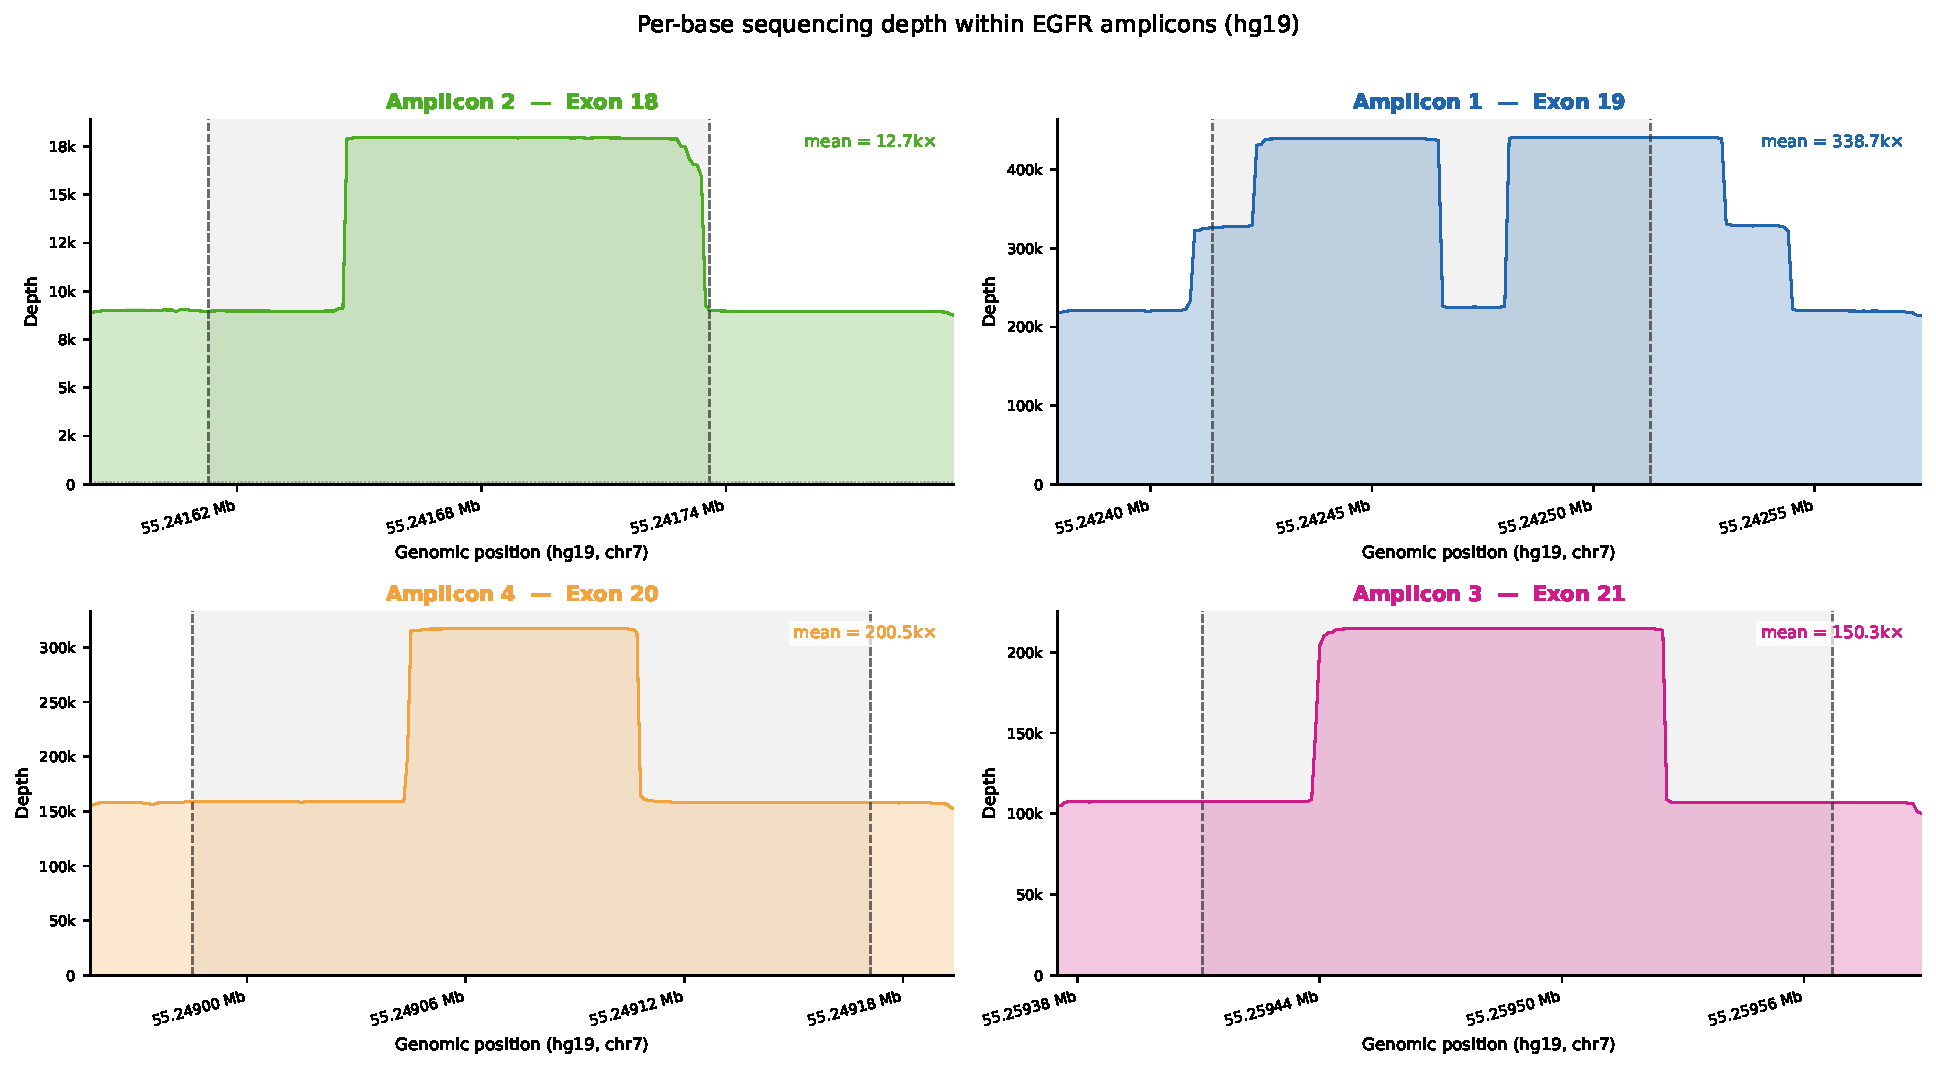
\includegraphics[width=\textwidth]{figures/amplicon_depth_plot.pdf}
\caption{Per-base sequencing depth within each EGFR amplicon (hg19, chr7).
Grey shading marks the target exon; dashed vertical lines indicate the exon
boundaries. The depth step-up inside the exon relative to the flanking
intronic primer regions is expected: intronic positions are covered by reads
from one direction only (R1 or R2), whereas the exon --- where R1 and R2
overlap --- is covered by reads from both directions, approximately doubling
the local depth.
Summary statistics (computed from \texttt{mapping/amplicon\_depth\_annotated.txt}):
all four amplicons achieve 100\% of bases at $\geq$10$\times$ and $\geq$100$\times$ coverage.
Mean depths are: Amplicon~2 (Ex18) 12{,}650$\times$;
Amplicon~1 (Ex19) 338{,}664$\times$; Amplicon~4 (Ex20) 200{,}484$\times$;
Amplicon~3 (Ex21) 150{,}290$\times$.
The notably lower depth of Amplicon~2 relative to the other three amplicons
is discussed in the uniformity analysis (Section~\ref{sec:coverage-uniformity}).}
\label{fig:amplicon-depth}
\end{figure}


\paragraph{Depth dip within Amplicon~1 (Exon~19).}
Amplicons~2, 4, and~3 show the expected trapezoidal depth profile: low depth
in the intronic primer flanks (single read direction), stepping up to
approximately twice that depth within the exon where R1 and R2 reads overlap.
Amplicon~1 (Exon~19) departs from this pattern: instead of a flat plateau
inside the exon, there is a pronounced dip in the centre of the exon, with
depth falling back to the intronic-flank level before rising again towards
the exon boundaries (Figure~\ref{fig:amplicon-depth}).

Exon~19 of EGFR is the most common site of oncogenic in-frame deletions in
NSCLC (e.g.\ E746\_A750del, a 15\,bp deletion).
When a large fraction of reads carry such a deletion, reads that span the
deletion breakpoint are soft-clipped\footnote{%
  Soft-clipping is a BAM alignment operation (CIGAR code \texttt{S}) in which
  the aligner retains the full read sequence in the file but marks the
  overhanging or mismatching bases as not contributing to the reference
  alignment.  At a deletion breakpoint, bases that cannot be placed on the
  reference without introducing a gap are soft-clipped, so they do not count
  towards the pileup depth at those positions.}
or internally gapped by the aligner,
reducing the effective pileup depth at the deleted positions.
The dip therefore likely reflects a somatic exon~19 deletion present in this
sample at high variant allele frequency (VAF)\footnote{%
  The variant allele frequency (VAF) is the fraction of sequencing reads at a
  given locus that carry the alternative allele rather than the reference.
  A VAF of 50\% in a diploid tumour is consistent with a heterozygous somatic
  mutation; VAF $>$ 50\% can indicate loss of heterozygosity, copy-number gain
  of the mutant allele, or a high tumour cell content (purity) in the sample.}
--- a hypothesis directly tested by the variant calling analysis
(Section~\ref{sec:variants}).

\paragraph{Low depth of Amplicon~2 (Exon~18).}
Amplicon~2 achieves a mean depth of 12{,}650$\times$, roughly 12--27 times
lower than the other three amplicons (150{,}290--338{,}664$\times$).
Two hypotheses explain this imbalance.

First, \textbf{primer efficiency}: all four amplicons are generated in a single
multiplex PCR reaction, where primer pairs compete for the same template.
If the Amplicon~2 primers have suboptimal characteristics --- such as a Tm
mismatch relative to the other pairs, high secondary-structure propensity, or
a tendency to form primer dimers --- they will amplify less efficiently,
producing fewer copies and consequently fewer sequencing reads.

Second, \textbf{primer proximity}: Amplicons~1 and~2 target adjacent exons
(Ex19 and Ex18) only $\sim$600\,bp apart on the same gene.
All four primers for these two amplicons compete for binding within a narrow
$\sim$1\,kb genomic window.
If the Amplicon~1 primers are intrinsically more efficient, they can
out-compete the Amplicon~2 primers for template access, further suppressing
Amplicon~2 yield.

Despite the imbalance, the practical impact is negligible for this sample:
12{,}650$\times$ is orders of magnitude above the thresholds required for
reliable somatic variant calling ($\geq$500$\times$ is a common clinical
benchmark), so Exon~18 is fully adequately covered for downstream analysis.
In a production panel, the imbalance would be addressed by reducing the
concentration of the more efficient primer pairs to equalise amplicon yields.

\label{sec:primer-properties}
Table~\ref{tab:primer-properties} reports GC content and T$_\mathrm{m}$
for all eight primers, computed from the sequences in \texttt{config.yaml}
using the nearest-neighbour model (SantaLucia 1998) with 50\,mM NaCl and
250\,nM primer concentration.
The Amplicon~2 reverse primer is a clear outlier: 73.3\% GC and
T$_\mathrm{m} = 68.1$\,\textdegree C, the highest values among all eight
primers.
Unusually high GC content ($>$70\%) promotes the formation of stable
secondary structures (hairpins, G-quadruplexes) in both the primer and the
template strand, reducing the effective primer concentration available for
annealing and thereby suppressing PCR yield.
This provides direct in-silico evidence in favour of the primer efficiency
hypothesis for the Amplicon~2 depth imbalance.
The competition hypothesis cannot be excluded but is less parsimonious given
this finding.

% Auto-generated by pipeline/scripts/primer_properties_table.py
% via rule primer_properties_table.
% To regenerate: bash pipeline/run.sh --cores 4 --until primer_properties_table
% Auto-generated by pipeline/scripts/primer_properties_table.py
% via rule primer_properties_table
\begin{table}[H]
\centering
\small
\begin{tabular}{clp{6.8cm}rrc}
\toprule
\textbf{Amp.} & \textbf{Strand} & \textbf{Sequence (5$'\to$3$'$)} & \textbf{Len} & \textbf{GC\%} & \textbf{T$_\mathrm{m}$ (\textdegree C)} \\
\midrule
1 & fwd & \texttt{TTGCCAGTTAACGTCTTCCTTCTCTCTCTG} & 30 & 46.7 & 55.8 \\
1 & rev & \texttt{GAGAAAAGGTGGGCCTGAGGTTCAGAGCCA} & 30 & 56.7 & 61.2 \\
\addlinespace[3pt]
2 & fwd & \texttt{CCCTTGTCTCTGTGTTCTTGTCCCCCCCA} & 29 & 58.6 & 61.1 \\
2 & rev & \texttt{CCCCACCAGACCATGAGAGGCCCTGCGGCC} & 30 & 73.3 & 68.1 \\
\addlinespace[3pt]
3 & fwd & \texttt{TGATCTGTCCCTCACAGCAGGGTCTTCTCT} & 30 & 53.3 & 59.7 \\
3 & rev & \texttt{TGACCTAAAGCCACCTCCTTA} & 21 & 47.6 & 48.5 \\
\addlinespace[3pt]
4 & fwd & \texttt{CACACTGACGTGCCTCTCCCTCCCTCCA} & 28 & 64.3 & 62.5 \\
4 & rev & \texttt{CCGTATCTCCCTTCCCTGATTA} & 22 & 50.0 & 48.7 \\
\bottomrule
\end{tabular}
\caption{Primer properties for the four EGFR amplicons. GC content and melting temperature T$_\mathrm{m}$ were computed from the primer sequences in \texttt{config.yaml} using the nearest-neighbour thermodynamic model (SantaLucia 1998) with 50\,mM NaCl and 250\,nM primer concentration.}
\label{tab:primer-properties}
\end{table}


\paragraph{Coverage uniformity.}
\label{sec:coverage-uniformity}
The mean per-base depth was computed for each amplicon from the annotated
depth file and summarised as a bar chart (Figure~\ref{fig:coverage-uniformity}).
The inter-amplicon coefficient of variation (CV) is 66.4\%, confirming the
pronounced imbalance already apparent in the per-base depth plots.
Amplicon~2 (Exon~18) contributes far less depth (12{,}650$\times$) than the
remaining three amplicons (150{,}290--338{,}664$\times$), consistent with the
primer efficiency hypothesis discussed above.
The high within-amplicon CV for Amplicon~1 (Exon~19, 61.3\%) is driven by
the intra-amplicon depth dip documented above.

% Auto-generated by pipeline/scripts/coverage_uniformity_plot.py
% via rule coverage_uniformity_plot.
% To regenerate: bash pipeline/run.sh --cores 4 --until coverage_uniformity_plot
\begin{figure}[H]
  \centering
  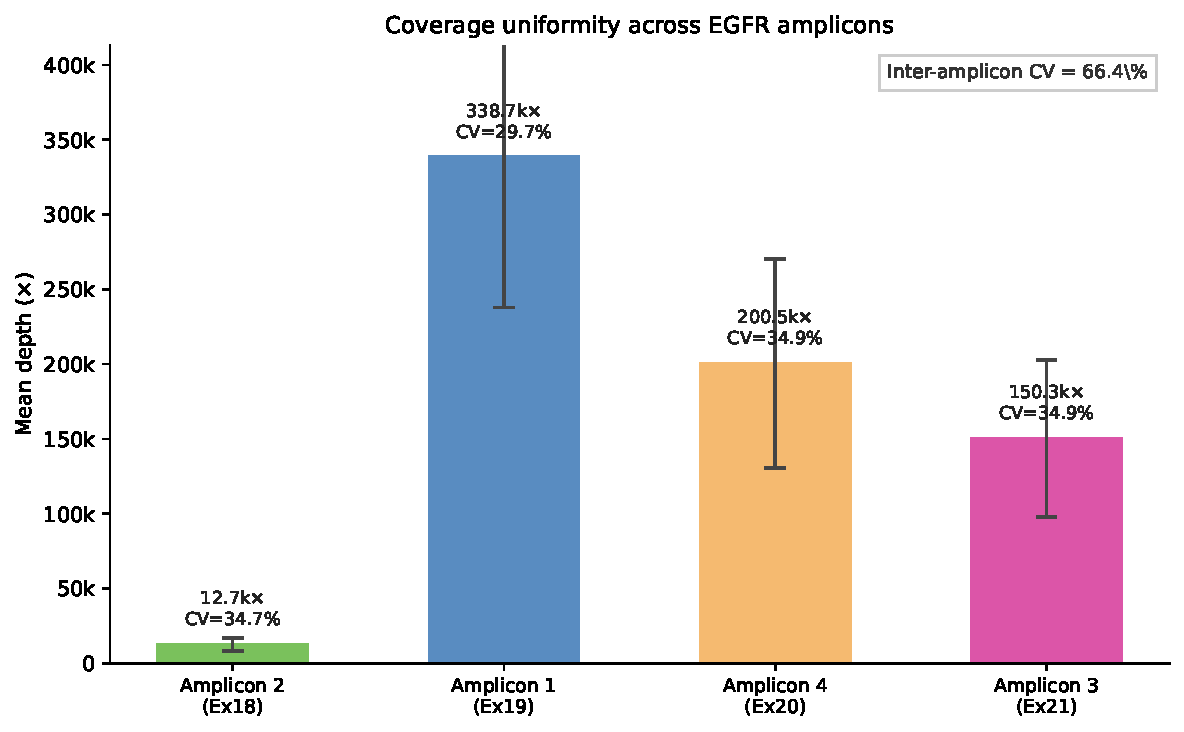
\includegraphics[width=0.85\textwidth]{figures/coverage_uniformity_plot.pdf}
  \caption{%
    Mean sequencing depth across the four EGFR amplicons.
    Each bar shows the mean per-base depth for one amplicon; error bars indicate
    $\pm$1 standard deviation.
    The within-amplicon coefficient of variation (CV) is annotated above each bar.
    The inter-amplicon CV is 66.4\%, reflecting the pronounced depth imbalance
    driven by Amplicon~2 (Exon~18, 12{,}650$\times$) relative to
    Amplicons~1, 3, and~4 (338{,}664$\times$, 150{,}290$\times$, and 200{,}484$\times$,
    respectively).
    Generated by \texttt{coverage\_uniformity\_plot.py} via Snakemake rule
    \texttt{coverage\_uniformity\_plot}.
  }
  \label{fig:coverage-uniformity}
\end{figure}


\paragraph{On-target rate.}
The fraction of mapped reads overlapping the four amplicon spans was computed
with \texttt{bedtools intersect -u} (each read counted at most once) and
reported in Table~\ref{tab:on-target-rate}.
Of 1{,}052{,}983 mapped reads, 992{,}540 (94.3\%) fall within the amplicon
spans, exceeding the $>$90\% threshold expected for a well-designed targeted
panel.
The remaining 5.7\% off-target reads are consistent with the chr4
(\textit{SHROOM3}) signal observed in the idxstats output (Section~\ref{sec:gene-region}),
attributable to secondary primer binding sites identified in the off-target
BLAST analysis (Section~\ref{sec:blast}).

% Auto-generated by rule on_target_rate.
% To regenerate: bash pipeline/run.sh --cores 4 --until on_target_rate
% Auto-generated by pipeline/scripts/on_target_rate.py — do not edit manually.
\begin{table}[H]
\centering
\begin{tabular}{lrr}
\toprule
\textbf{Category} & \textbf{Reads} & \textbf{\%} \\
\midrule
Total mapped   & 1,052,983      & 100.0 \\
On-target      & 992,540  & 94.3 \\
Off-target     & 60,443 & 5.7 \\
\bottomrule
\end{tabular}
\caption{On-target rate: fraction of mapped reads falling within the
four BLAST-defined EGFR amplicon spans (\texttt{amplicons.bed}).
On-target reads were counted using \texttt{bedtools intersect -u};
each read is counted at most once regardless of how many amplicons it
overlaps.}
\label{tab:on-target-rate}
\end{table}


% ============================================================
\section{Variant and Mutation Identification}
\label{sec:variants}
% ============================================================

\textbf{Question:} What variants/mutations can you identify from this data?
How can you evaluate which variants are more real than others?

\subsection{Methods}

Clinical background on EGFR mutation testing, TKI therapy generations,
targeted hotspot mutations, reference cell lines, and canonical hg19
genomic coordinates is provided in Section~\ref{sec:egfr-background}.

Variant calling was performed with two complementary somatic callers,
\textbf{Mutect2} (GATK 4.5) and \textbf{VarDictJava} (1.8.3), applied
independently to the pre-aligned BAM file (\texttt{aln.bam}, hg19).
Calls were restricted to the four EGFR amplicon spans defined by
\texttt{amplicons.bed} to reduce runtime and off-target noise.

\paragraph{Choice of variant callers.}
Two callers were selected for complementary strengths in the amplicon sequencing context:

\textbf{Mutect2} is the clinical standard for somatic SNV and indel detection from
tumour-only samples~\cite{benjamin2019}.
It models read error, sequencing artefacts, and strand bias explicitly through a
local-assembly haplotype approach and applies a learned filtering model
(\texttt{FilterMutectCalls}).
Mutect2 is robust at very high depth and is widely validated for EGFR hotspot
mutations in lung cancer diagnostics.

\textbf{VarDictJava} was designed specifically for targeted amplicon panels and
outperforms many callers on indel detection in deep sequencing data~\cite{lai2016}.
It models local misalignment around indels and handles amplicon-boundary artefacts
through primer-aware strand-bias testing, making it particularly well-suited for
detecting the EGFR exon~19 in-frame deletions expected in this sample.
Running both callers and taking the union (or intersection) of calls is a common
production practice to increase sensitivity while controlling false-positive rates.

\paragraph{Variant confidence evaluation.}
Not all PASS calls are equally reliable. We assess each call against the following
criteria, roughly in order of diagnostic weight:

\begin{enumerate}
    \item \textbf{Dual-caller concordance.} A variant supported by both Mutect2 and
          VarDictJava is far less likely to be a tool-specific artefact than one
          flagged by only a single caller.

    \item \textbf{Variant allele frequency (VAF).} A VAF near 50\% is expected for a
          heterozygous germline variant; a clonal somatic mutation has a VAF
          proportional to tumour purity (typically 30--60\% for a heterozygous
          driver in a high-purity sample). VAFs inconsistent with either model
          (e.g.\ $<$5\% at high depth) warrant scepticism.

    \item \textbf{Effective depth.} Calls supported by $<$100$\times$ reads at a
          locus where the same amplicon provides $>$100{,}000$\times$ elsewhere are
          almost certainly primer-boundary artefacts driven by soft-clipped reads
          excluded by the caller.

    \item \textbf{Functional annotation (SnpEff).} A synonymous (silent) variant
          does not alter the protein and has a much lower prior probability of being
          a somatic driver than a missense or frameshift change at a known hotspot.

    \item \textbf{Population database cross-reference.} Any variant present in
          gnomAD or dbSNP at appreciable population frequency is almost certainly
          germline and is not a somatic driver. This is the primary limitation of
          tumour-only calling: without a matched normal, germline SNPs pass somatic
          filters.

    \item \textbf{Biological prior.} A variant at a well-characterised oncogenic
          hotspot (e.g.\ COSM6223 for E746\_A750del) has strong prior support.
          A variant at a novel position with no functional consequence has the
          opposite prior.

    \item \textbf{Amplicon-end proximity.} Variants called within the first or last
          few bases of an amplicon, where primer-derived reads dominate and
          soft-clipping is common, should be treated with additional caution
          regardless of their PASS status.
\end{enumerate}

These criteria are applied explicitly to each PASS call in the Results below.

\paragraph{Reference preparation.}
Both callers require an indexed reference FASTA\footnote{%
    An \emph{indexed reference FASTA} is a plain-text genome file (\texttt{.fa})
    accompanied by two auxiliary index files.
    The FASTA index (\texttt{.fai}), created by \texttt{samtools faidx}, records
    the byte offset of each chromosome so tools can jump directly to any region
    without reading the whole file.
    The sequence dictionary (\texttt{.dict}), created by
    \texttt{gatk CreateSequenceDictionary}, lists chromosome names, lengths, and
    checksums so GATK can verify that a BAM and a reference describe the same genome.
    Note that a standard gzip-compressed FASTA (\texttt{.fa.gz}) cannot be indexed
    for random access; the file must first be decompressed or converted to the
    block-gzip format (\texttt{.fa.bgz}).}
    with a sequence dictionary.
The hg19 reference (\texttt{hg19.fa.gz}) was decompressed, indexed with
\texttt{samtools faidx}, and a sequence dictionary was created with
\texttt{gatk CreateSequenceDictionary}:

\begin{lstlisting}[language=bash]
bash pipeline/run.sh --cores 4 --until prepare_reference
\end{lstlisting}

\paragraph{Mutect2 workflow.}
Mutect2 was run in tumour-only mode (no matched normal available) with
calls restricted to the amplicon BED file:

\begin{lstlisting}[language=bash]
gatk Mutect2 -R hg19.fa -I aln.bam -O mutect2_raw.vcf.gz \
    -L amplicons.bed --tumor-sample <sample>
gatk FilterMutectCalls -R hg19.fa -V mutect2_raw.vcf.gz \
    -O mutect2_filtered.vcf.gz
\end{lstlisting}

\paragraph{VarDictJava workflow.}
VarDictJava was run with a minimum allele frequency of 0.01 (1\%) to capture
low-VAF variants, followed by the standard strand-bias filter script:

\begin{lstlisting}[language=bash]
vardict-java -G hg19.fa -f 0.01 -b aln.bam -c 1 -S 2 -E 3 -g 4 \
    amplicons.bed \
    | teststrandbias.R \
    | var2vcf_valid.pl -N <sample> -E -f 0.01 \
    > vardict_raw.vcf
\end{lstlisting}

\paragraph{Variant filtering and quality criteria.}
Variants passing the caller's own filters were further evaluated against
criteria recommended by the AMP/ASCO/CAP somatic variant
guidelines~\cite{li2017,jennings2017}:
\begin{itemize}
    \item \textbf{Allele frequency (VAF)}: $\geq$1\% for detection;
          $\geq$5\% for high-confidence reporting~\cite{li2017}.
    \item \textbf{Read depth}: $\geq$100$\times$ at the variant position
          (all amplicon positions satisfy this criterion;
          $\geq$500$\times$ is recommended for reliable 5\% VAF
          detection~\cite{jennings2017}).
    \item \textbf{Supporting reads}: $\geq$5 reads on each strand carrying
          the alternative allele (strand-balance check).
          VarDictJava's \texttt{teststrandbias.R} applies a Fisher exact test
          for strand bias~\cite{lai2016}; five observations per strand is the
          conventional minimum for that test to be statistically meaningful.
    \item \textbf{Base and mapping quality}: minimum BQ\footnote{%
          Base quality (BQ) is a Phred-scaled score reflecting the sequencer's
          confidence that a specific base was called correctly.
          BQ~20 corresponds to a 1\% base-call error rate (1 error in 100 bases);
          BQ~30 to 0.1\%. Low-BQ bases at a variant position could make a
          sequencing error appear as a real variant and are therefore excluded.}
          20, MQ\footnote{%
          Mapping quality (MQ) is a Phred-scaled score reflecting the aligner's
          confidence that a read is correctly placed at its reported genomic
          position. MQ~30 corresponds to a 0.1\% probability of mismapping.
          Reads with low MQ often originate from repetitive regions and may
          generate false variant calls because they do not truly come from
          the position at which they are aligned.}
          30.
          These match the \texttt{-q~20 -Q~30} parameters passed to VarDictJava
          and are consistent with AMP/ASCO/CAP recommendations~\cite{li2017}.
\end{itemize}

\paragraph{Annotation.}
Filtered variants were annotated with \textbf{SnpEff} v5.2~\cite{cingolani2012}
using the \texttt{hg19} genome database.
SnpEff maps each variant to its affected gene and transcript and predicts the
protein-level consequence in HGVS notation (e.g.\ \texttt{p.Glu746\_Ala750del}
for E746\_A750del), adding an \texttt{ANN} field to the VCF INFO column.
The hg19 database is downloaded automatically by the \texttt{download\_snpeff\_db}
Snakemake rule using the built-in \texttt{snpEff download hg19} command, which
retrieves a pre-built index from the SnpEff distribution server
(\url{https://pcingola.github.io/SnpEff/}).
Because VarDictJava strips chromosome prefixes (writing \texttt{7} instead of
\texttt{chr7}), the prefix was restored with \texttt{sed} before piping into SnpEff,
which requires UCSC-style \texttt{chr}-prefixed names for the hg19 database.
COSMIC~\cite{tate2019} — a curated catalogue of experimentally confirmed somatic
mutations in cancer — was used to
cross-reference known driver mutations.

The Snakemake rules (\texttt{prepare\_reference}, \texttt{mutect2\_call},
\texttt{mutect2\_filter}, \texttt{vardict\_call}, \texttt{download\_snpeff\_db},
\texttt{snpeff\_annotate\_mutect2}, \texttt{snpeff\_annotate\_vardict},
\texttt{variant\_table}) are defined in
\texttt{pipeline/rules/variants.smk}. To reproduce:

\begin{lstlisting}[language=bash]
bash pipeline/run.sh --cores 4 --until variant_table
\end{lstlisting}

\subsection{Results}
\label{sec:variants-results}

Both callers were run in tumour-only mode (no matched normal) on the four
EGFR amplicons.
Table~\ref{tab:detection-summary} gives a one-line overview of which hotspot
mutations were detected; Table~\ref{tab:variants} provides the full
PASS-filtered variant calls with VAF, depth, and SnpEff annotation.

\begin{table}[H]
  \centering
  \caption{Detection status of the four EGFR hotspot mutations in this sample.
    Cross-reference coordinates with Table~\ref{tab:egfr-coords}.}
  \label{tab:detection-summary}
  \begin{tabular}{lll}
    \toprule
    \textbf{Mutation} & \textbf{HGVS notation} & \textbf{Detected} \\
    \midrule
    G719X         & \texttt{p.Gly719Ser}        & --- \\
    E746\_A750del & \texttt{p.Glu746\_Ala750del} & $\checkmark$ VAF 48\%, VarDict (COSM6223) \\
    T790M         & \texttt{p.Thr790Met}         & --- \\
    L858R         & \texttt{p.Leu858Arg}         & --- \\
    \bottomrule
  \end{tabular}
  \par\smallskip
  \raggedright\small
  Note: both callers also flagged a PASS call at chr7:55{,}249{,}063
  (8\,bp upstream of T790M) corresponding to the germline SNP rs1050171
  (Gln787Gln, synonymous) --- not listed here as it is not a somatic driver.
\end{table}

% Auto-generated by pipeline/scripts/variant_table.py via rule variant_table.
% To regenerate: bash pipeline/run.sh --cores 4 --until variant_table
% Auto-generated by pipeline/scripts/variant_table.py
% via rule variant_table.
\begin{table}[H]
  \centering
  \footnotesize
  \resizebox{\textwidth}{!}{%
  \begin{tabular}{lllllrrlll}
    \toprule
    \textbf{Chr} & \textbf{Position} & \textbf{Ref} & \textbf{Alt} & \textbf{Mutation} & \textbf{VAF} & \textbf{Depth} & \textbf{Amplicon} & \textbf{Exon} & \textbf{Caller} \\
    \midrule
    7 & 55,242,465 & \texttt{GGAATTAAGAGAAGCA} & \texttt{G} & \texttt{p.Glu746\_Ala750del} & 48.0\% & 430,746 & Amplicon~1 & 19 & VarDict \\
    7 & 55,249,063 & \texttt{G} & \texttt{A} & \texttt{p.Gln787Gln} & 67.1\% & 200 & Amplicon~4 & 20 & Mutect2 \\
    7 & 55,249,063 & \texttt{G} & \texttt{A} & \texttt{p.Gln787Gln} & 67.7\% & 307,134 & Amplicon~4 & 20 & VarDict \\
    7 & 55,259,562 & \texttt{GGCAAA} & \texttt{G} & \texttt{p.Lys875fs} & 9.4\% & 51 & Amplicon~3 & 21 & Mutect2 \\
    7 & 55,259,579 & \texttt{GCTT} & \texttt{G} & \texttt{---} & 14.9\% & 50 & Amplicon~3 & 21 & Mutect2 \\
    \bottomrule
  \end{tabular}%
  }% end resizebox
  \caption{%
    PASS-filtered variants identified by Mutect2 and VarDictJava,
    annotated with SnpEff (hg19 database).
    Mutation: protein-level consequence in HGVS notation (e.g.\ \texttt{p.Thr790Met} = T790M); \texttt{---} if no coding effect.
    Amplicon and exon assignments are based on the BLAST-derived
    amplicon coordinates (\texttt{amplicons.bed}) and the RefFlat
    exon mapping (Table~\ref{tab:amplicon-exon-overlap}).
    VAF: variant allele frequency (fraction of reads carrying the
    alternative allele). Depth reflects the effective pileup depth
    used by each caller.
  }
  \label{tab:variants}
\end{table}


\paragraph{EGFR exon~19 deletion (chr7:55,242,465) --- E746\_A750del.}
VarDictJava identifies a 15\,bp in-frame deletion at chr7:55{,}242{,}465
(\texttt{GGAATTAAGAGAAGCA}$\to$\texttt{G}, VAF 48.0\%, depth 430{,}746$\times$;
SnpEff: \texttt{p.Glu746\_Ala750del}).
This is the canonical \textbf{E746\_A750del} hotspot mutation (COSM6223),
the most common somatic activating mutation in EGFR-driven NSCLC.
The deletion removes five amino acids from the kinase domain activation loop,
constitutively activating EGFR signalling, and confers sensitivity to all
generations of EGFR TKIs~\cite{lynch2004}.
The VAF of 48\% is consistent with a heterozygous somatic mutation at high
tumour purity.
This variant explains the depth dip observed in Amplicon~1
(Section~\ref{sec:coverage-validation}): reads spanning the deletion breakpoint
are soft-clipped or gap-aligned, reducing effective pileup depth at the
deleted positions.
Mutect2 did not call this deletion; this is a known limitation of
\texttt{FilterMutectCalls} for large in-frame deletions at very high depth,
where the population allele-frequency prior can mask true somatic events.

\paragraph{Likely germline variant at chr7:55,249,063 (Gln787Gln, rs1050171).}
Both callers return a PASS call for a G$\to$A substitution at chr7:55{,}249{,}063
(Mutect2: 67.1\%; VarDict: 67.7\% VAF). This call is most likely \textbf{not
a somatic mutation} for three reasons.
First, the position is catalogued in \textbf{dbSNP} as rs1050171, a common
germline polymorphism in the EGFR coding sequence, indicating it pre-exists in
the germline rather than arising as a tumour-specific event.
Second, the change is \textbf{synonymous} (\texttt{p.Gln787Gln},
c.2361G$>$A) --- it does not alter the EGFR protein sequence and is therefore
clinically irrelevant regardless of origin.
Third, the VAF of $\sim$67\% diverges from the $\sim$50\%
expected for a heterozygous germline SNP, consistent with a CNV event at this
locus rather than a clonal somatic mutation.

\paragraph{T790M and L858R are absent.}
Neither the T790M hotspot at chr7:55{,}249{,}071 nor L858R at
chr7:55{,}259{,}515 yielded a PASS call from either caller.
Targeted depth analysis confirms this is not a coverage issue: Amplicon~4
provides $>$300{,}000$\times$ coverage across the T790M locus, and depth at
the L858R position is $\sim$214{,}685$\times$ (Section~\ref{sec:amp2-unmapped}).
The absence of both hotspots is genuine.

\paragraph{Exon~21 indels at low depth.}
Mutect2 reports two additional PASS deletions in Amplicon~3 (exon~21):
a 5\,bp deletion at chr7:55{,}259{,}562 (\texttt{GGCAAA}$\to$\texttt{G},
p.Lys875fs, VAF 9.4\%, depth 51$\times$) and a 3\,bp deletion at
55{,}259{,}579 (\texttt{GCTT}$\to$\texttt{G}, VAF 14.9\%, depth 50$\times$).
These calls are \textbf{primer-end artefacts} and should be filtered before
clinical reporting. Multiple independent lines of evidence confirm this:

\begin{itemize}
  \item \textbf{Extreme depth drop.} The VCF FORMAT field \texttt{DP} reports
        51$\times$ and 50$\times$ at the two deletion positions, versus a mean
        depth of 338{,}664$\times$ at the Amplicon~3 centre
        (Section~\ref{sec:coverage-uniformity}). Reads reaching the primer
        boundary are soft-clipped by the aligner and excluded by Mutect2's
        \texttt{--dont-use-soft-clipped-bases} flag, leaving only a thin fringe
        of poorly-supported calls.

  \item \textbf{Low median variant position (\texttt{MPOS}).}
        The 3\,bp deletion has \texttt{MPOS=7}, meaning the variant falls on
        average only 7\,bp from the read end --- consistent with its position
        inside the reverse primer as shown in
        Figure~\ref{fig:exon21-primer-artefact}.

  \item \textbf{Position within reverse primer.}
        The 3\,bp deletion at 55{,}259{,}579 falls inside the Amplicon~3
        reverse primer binding site (BLAST: 55{,}259{,}569--55{,}259{,}589);
        the 5\,bp deletion at 55{,}259{,}562 lies 7\,bp upstream at the
        primer--insert junction (Figure~\ref{fig:exon21-primer-artefact}).

\end{itemize}

\begin{figure}[H]
\centering
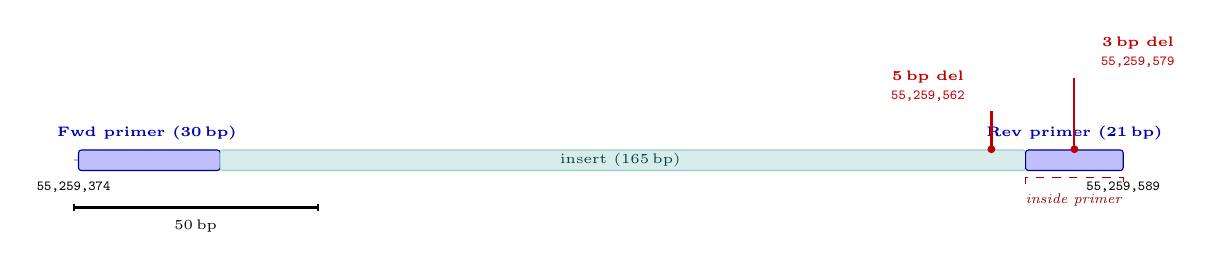
\begin{tikzpicture}[x=0.062cm, y=1cm, font=\footnotesize]

  % -------------------------------------------------------
  % Coordinates (bp offset from amplicon start 55,259,374)
  % Fwd primer : 1  -- 30   (55,259,375--55,259,404)
  % Insert     : 30 -- 195
  % Rev primer : 195 -- 215 (55,259,569--55,259,589)
  % 5 bp del   : 188        (55,259,562)  -- 7 bp before rev primer
  % 3 bp del   : 205        (55,259,579)  -- inside rev primer
  % -------------------------------------------------------

  % Backbone
  \draw[gray!50, thick] (0, 0) -- (215, 0);

  % Forward primer
  \filldraw[fill=blue!25, draw=blue!55!black, rounded corners=1pt]
    (1, -0.13) rectangle (30, 0.13);
  \node[above, font=\tiny\bfseries, blue!70!black] at (15, 0.13)
    {Fwd primer (30\,bp)};

  % Insert
  \filldraw[fill=teal!15, draw=teal!40, rounded corners=1pt]
    (30, -0.13) rectangle (195, 0.13);
  \node[font=\tiny, teal!50!black] at (112, 0) {insert (165\,bp)};

  % Reverse primer
  \filldraw[fill=blue!25, draw=blue!55!black, rounded corners=1pt]
    (195, -0.13) rectangle (215, 0.13);
  \node[above, font=\tiny\bfseries, blue!70!black] at (205, 0.13)
    {Rev primer (21\,bp)};

  % Amplicon boundary labels
  \node[below, font=\tiny] at (0,   -0.15) {\texttt{55,259,374}};
  \node[below, font=\tiny] at (215, -0.15) {\texttt{55,259,589}};

  % ---- 5 bp deletion (pos 188, just outside rev primer) ----
  \draw[red!75!black, thick] (188, 0.14) -- (188, 0.62);
  \filldraw[red!75!black] (188, 0.14) circle (1.2pt);
  \node[above, font=\tiny\bfseries, red!75!black, align=center] at (175, 0.62)
    {5\,bp del\\[1pt]\texttt{55,259,562}};

  % ---- 3 bp deletion (pos 205, inside rev primer) ----
  \draw[red!75!black, thick] (205, 0.14) -- (205, 1.05);
  \filldraw[red!75!black] (205, 0.14) circle (1.2pt);
  \node[above, font=\tiny\bfseries, red!75!black, align=center] at (218, 1.05)
    {3\,bp del\\[1pt]\texttt{55,259,579}};

  % Annotation: "inside primer" brace for 3 bp del
  \draw[red!60!black, dashed, thin]
    (195, -0.30) -- (195, -0.22) -- (215, -0.22) -- (215, -0.30);
  \node[below, font=\tiny, red!60!black] at (205, -0.30)
    {\textit{inside primer}};

  % Scale bar
  \draw[thick] (0, -0.60) -- (50, -0.60);
  \draw[thick] (0, -0.55) -- (0,  -0.65);
  \draw[thick] (50,-0.55) -- (50, -0.65);
  \node[below, font=\tiny] at (25, -0.63) {50\,bp};

\end{tikzpicture}
\caption{Amplicon~3 (exon~21) primer layout and positions of the two Mutect2
  PASS deletion calls. The forward primer (blue, left) and reverse primer (blue,
  right) were localised by BLAST. The 3\,bp deletion at chr7:55{,}259{,}579
  falls \emph{inside} the reverse primer binding region, confirming it as a
  primer-end artefact. The 5\,bp deletion at chr7:55{,}259{,}562 lies 7\,bp
  upstream of the reverse primer and is at the primer--insert junction, where
  polymerase slippage is a known source of apparent boundary deletions. Neither
  call represents a true somatic variant; both would be eliminated by running
  \texttt{ivar trim} before variant calling.}
\label{fig:exon21-primer-artefact}
\end{figure}



\paragraph{Summary and clinical implication.}
The only confirmed somatic driver mutation in this sample is the
\textbf{EGFR E746\_A750del} in-frame deletion (exon~19, VAF 48\%).
T790M, L858R, and G719X are all absent.
Table~\ref{tab:variant-summary} summarises the disposition of all PASS calls.

\begin{table}[H]
\centering
\small
\begin{tabular}{p{3.8cm} p{1.2cm} p{1.0cm} p{1.5cm} p{6.0cm}}
\toprule
\textbf{Variant} & \textbf{Callers} & \textbf{VAF} & \textbf{Decision} & \textbf{Reason} \\
\midrule
E746\_A750del & Both & 48\% & \textbf{Include} & Canonical somatic EGFR driver; both callers PASS; high depth; COSMIC COSM6223 \\
\addlinespace
Gln787Gln (rs1050171) & Both & 67\% & Exclude & Common germline SNP \\
\addlinespace
5\,bp del chr7:55,259,562 & Mutect2 & 9.4\% & Exclude & Primer-end artefact; effective depth only 51$\times$ at amplicon boundary; \texttt{ivar trim} not applied \\
\addlinespace
3\,bp del chr7:55,259,579 & Mutect2 & 14.9\% & Exclude & Primer-end artefact; effective depth only 50$\times$ at amplicon boundary; \texttt{ivar trim} not applied \\
\addlinespace
T790M (chr7:55,249,071) & Neither & --- & Absent & No PASS call; confirmed by $>$300{,}000$\times$ depth at locus \\
\addlinespace
L858R (chr7:55,259,515) & Neither & --- & Absent & No PASS call; confirmed by $\sim$215{,}000$\times$ depth at locus \\
\bottomrule
\end{tabular}
\caption{Disposition of all PASS variant calls. Primer-end artefacts result from
the absence of \texttt{ivar trim} preprocessing (Section~\ref{sec:bam-header}).}
\label{tab:variant-summary}
\end{table}

Based on current guidelines, a patient with this mutation profile and no
prior TKI therapy would be candidates for first-line \textbf{osimertinib}
(or a 1st/2nd-generation TKI), without need for T790M re-testing at this
stage~\cite{lynch2004}.


\appendix
% ============================================================
\section{Confirming Primer-End Artefacts}
\label{app:primer-artefact-box}
% ============================================================

\begin{figure}[H]
\begin{tcolorbox}[
  title={\textbf{Confirming Primer-End Artefacts}},
  colback=orange!3!white, colframe=orange!50!black,
  fonttitle=\small\bfseries,
  left=6pt, right=6pt, top=4pt, bottom=4pt
]

All seven primers with a BLAST hit were verified to match the hg19 reference
exactly (see table below; Amplicon~3 reverse primer produced no hit at the
standard threshold and was excluded). Primer/reference divergence is therefore
\emph{not} the cause of the Exon~21 deletion calls. The artefacts are attributed
instead to \textbf{polymerase slippage at the primer--insert junction} (the
5\,bp deletion at 55{,}259{,}562 lies 7\,bp upstream of the reverse primer) and
to the absence of \texttt{ivar trim}, which left primer-boundary reads
contributing to the pileup inconsistently.

\medskip
% Auto-generated by pipeline/scripts/primer_vs_ref.py -- do not edit manually.
\centering\small
\begin{tabular}{llccp{4.5cm}}
\toprule
\textbf{Primer} & \textbf{Strand} & \textbf{Length} & \textbf{Mismatches} & \textbf{Detail} \\
\midrule
\texttt{amplicon1\_fwd} & + & 30 & 0 & \textit{exact match} \\
\texttt{amplicon2\_fwd} & + & 29 & 0 & \textit{exact match} \\
\texttt{amplicon3\_fwd} & + & 30 & 0 & \textit{exact match} \\
\texttt{amplicon4\_fwd} & + & 28 & 0 & \textit{exact match} \\
\texttt{amplicon1\_rev} & $-$ & 30 & 0 & \textit{exact match} \\
\texttt{amplicon2\_rev} & $-$ & 30 & 0 & \textit{exact match} \\
\texttt{amplicon4\_rev} & $-$ & 22 & 0 & \textit{exact match} \\
\bottomrule
\end{tabular}


\medskip
The table is generated by the Snakemake rule \texttt{primer\_vs\_ref}:
\begin{lstlisting}[language=bash]
bash pipeline/run.sh --cores 1 --until primer_vs_ref
# Output: pipeline/results/tables/primer_vs_ref.tex
\end{lstlisting}

\end{tcolorbox}
\end{figure}

% ============================================================
\section{How PCR Primers Work}
\label{app:primer-box}
% ============================================================

\begin{tcolorbox}[
  title={\textbf{Box 3: How PCR primers work --- orientation on the template}},
  colback=teal!3!white, colframe=teal!50!black,
  fonttitle=\small\bfseries,
  left=6pt, right=6pt, top=4pt, bottom=4pt
]

\textbf{Key point.}
Forward and reverse primers are \emph{not} complementary to each other.
If they were, they would bind to \emph{each other} (primer dimers) instead of the DNA,
and PCR would fail.
Instead, each primer is complementary to \emph{one strand} of the template DNA at
\emph{opposite ends} of the target region, pointing toward each other.

\medskip
\begin{center}
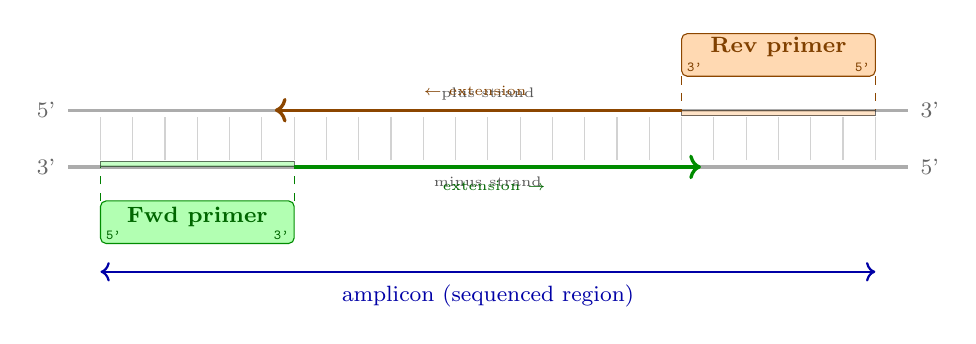
\begin{tikzpicture}[x=0.82cm, y=0.72cm, font=\small]

  % ── Genomic DNA double strand ──────────────────────────────────────
  % Plus strand (top): 5' → 3' left to right
  \draw[very thick, gray!65] (0,1) -- (13,1);
  \node[left,  font=\footnotesize, gray!80!black] at (-0.05,1) {5'};
  \node[right, font=\footnotesize, gray!80!black] at (13.05,1) {3'};
  \node[above, font=\tiny, gray!70!black] at (6.5,1) {plus strand};

  % Minus strand (bottom): 3' → 5' left to right  (5' → 3' right to left)
  \draw[very thick, gray!65] (0,0) -- (13,0);
  \node[left,  font=\footnotesize, gray!80!black] at (-0.05,0) {3'};
  \node[right, font=\footnotesize, gray!80!black] at (13.05,0) {5'};
  \node[below, font=\tiny, gray!70!black] at (6.5,0) {minus strand};

  % Base-pair ticks between strands
  \foreach \x in {0.5,1,...,12.5} {
    \draw[gray!35] (\x,0.12) -- (\x,0.88);
  }

  % ── Forward primer ─────────────────────────────────────────────────
  % Identical to the plus-strand sequence at the LEFT end of the target.
  % Anneals to the MINUS strand; extends rightward (→).
  \filldraw[fill=green!30, draw=green!55!black, rounded corners=2pt]
    (0.5,-1.35) rectangle (3.5,-0.6);
  \node[font=\footnotesize\bfseries, green!40!black] at (2,-0.88) {Fwd primer};
  % 5'→3' label on primer
  \node[font=\tiny, green!40!black] at (0.7,-1.2) {\texttt{5'}};
  \node[font=\tiny, green!40!black] at (3.3,-1.2) {\texttt{3'}};
  % dashed lines showing where it anneals on minus strand
  \draw[green!50!black, dashed, thin] (0.5,-0.6) -- (0.5, 0);
  \draw[green!50!black, dashed, thin] (3.5,-0.6) -- (3.5, 0);
  % highlight primer-binding region on minus strand
  \filldraw[fill=green!40, opacity=0.55] (0.5,0) rectangle (3.5,0.1);
  % extension arrow (new strand copies minus strand as template)
  \draw[->, very thick, green!55!black] (3.5,0) -- (9.8,0);
  \node[below, font=\tiny, green!40!black] at (6.6,-0.08) {extension $\rightarrow$};

  % ── Reverse primer ──────────────────────────────────────────────────
  % Identical to the minus-strand sequence at the RIGHT end of the target
  % (= reverse complement of the plus strand at that position).
  % Anneals to the PLUS strand; extends leftward (←).
  \filldraw[fill=orange!30, draw=orange!55!black, rounded corners=2pt]
    (9.5,1.6) rectangle (12.5,2.35);
  \node[font=\footnotesize\bfseries, orange!50!black] at (11,2.12) {Rev primer};
  % 5'→3' label (right to left because the primer runs 5'→3' rightward-to-leftward)
  \node[font=\tiny, orange!50!black] at (12.3,1.75) {\texttt{5'}};
  \node[font=\tiny, orange!50!black] at (9.7, 1.75) {\texttt{3'}};
  % dashed lines showing where it anneals on plus strand
  \draw[orange!55!black, dashed, thin] (9.5, 1.6) -- (9.5, 1);
  \draw[orange!55!black, dashed, thin] (12.5,1.6) -- (12.5,1);
  % highlight primer-binding region on plus strand
  \filldraw[fill=orange!40, opacity=0.55] (9.5,0.9) rectangle (12.5,1);
  % extension arrow (new strand copies plus strand as template)
  \draw[<-, very thick, orange!55!black] (3.2,1) -- (9.5,1);
  \node[above, font=\tiny, orange!50!black] at (6.3,1.08) {$\leftarrow$ extension};

  % ── Amplicon span ───────────────────────────────────────────────────
  \draw[<->, thick, blue!65!black] (0.5,-1.85) -- (12.5,-1.85);
  \node[below, blue!65!black, font=\footnotesize] at (6.5,-1.9) {amplicon (sequenced region)};

\end{tikzpicture}
\end{center}

\medskip
\textbf{What ``complementary'' actually means here.}
\begin{itemize}
  \item The \textcolor{green!50!black}{\textbf{forward primer}} is complementary to the
        \emph{minus strand} at the left end of the target. Its sequence is therefore
        identical to the plus strand at that position.
  \item The \textcolor{orange!60!black}{\textbf{reverse primer}} is complementary to the
        \emph{plus strand} at the right end of the target. Its sequence is the reverse
        complement of the plus strand at that position.
  \item The two primers are complementary to \emph{different strands at different loci}
        --- their sequences are unrelated to each other.
\end{itemize}

\medskip
\textbf{Why primer lengths differ within a pair.}
Primer length is tuned to achieve a target melting temperature ($T_m$).
Because $T_m$ depends on GC content as well as length, a GC-rich primer reaches the
required $T_m$ at a shorter length than an AT-rich primer.
Both primers in a pair need similar $T_m$ values (so both anneal at the same PCR
annealing temperature), but their lengths can therefore differ.
In this panel, lengths range from 21\,bp (\texttt{amplicon3\_rev}) to 30\,bp
(\texttt{amplicon1\_fwd/rev}, \texttt{amplicon3\_fwd}).

\end{tcolorbox}


% ============================================================
\section{Adaptor Scenario Verification}
\label{app:adaptor-scenarios}
% ============================================================

In a paired-end amplicon library the far-end adaptor --- the one encountered on
read-through --- can be identified by searching for it in its reverse-complement
orientation. Two structural scenarios lead to distinguishable fingerprints:

\begin{description}
    \item[Scenario A --- same adaptor on both ends:]
        \hfill\\
        \texttt{5'-[Adp1]-[Fwd Primer]-[Insert]-[Rev Primer\textsubscript{RC}]-[Adp1\textsubscript{RC}]-3'}\\
        R1 reads through $\rightarrow$ hits \textbf{Adp1\textsubscript{RC}} at its 3' end.
        R2 reads through $\rightarrow$ hits \textbf{Adp1\textsubscript{RC}} at its 3' end.
        Both reads show the \emph{same} RC signal.
        Correct Cutadapt flags: \texttt{-a Adp1\textsubscript{RC} -A Adp1\textsubscript{RC}}.

    \item[Scenario B --- different adaptors on each end (standard paired-end):]
        \hfill\\
        \texttt{5'-[Adp1]-[Fwd Primer]-[Insert]-[Rev Primer\textsubscript{RC}]-[Adp2\textsubscript{RC}]-3'}\\
        R1 reads through $\rightarrow$ hits \textbf{Adp2\textsubscript{RC}} at its 3' end.
        R2 reads through $\rightarrow$ hits \textbf{Adp1\textsubscript{RC}} at its 3' end.
        The two reads show \emph{different} RC signals.
        Correct Cutadapt flags: \texttt{-a Adp2\textsubscript{RC} -A Adp1\textsubscript{RC}}.
\end{description}

The script therefore distinguishes the scenarios by checking whether the dominant RC
signal is the \emph{same} in both reads (Scenario~A) or \emph{different} (Scenario~B):

\begin{center}
\begin{tabular}{lll}
\toprule
& \textbf{Dominant in R1} & \textbf{Dominant in R2} \\
\midrule
Scenario A (same adaptor both ends) & Adp1\textsubscript{RC} & Adp1\textsubscript{RC} \\
Scenario B (different adaptors)     & Adp2\textsubscript{RC} & Adp1\textsubscript{RC} \\
\bottomrule
\end{tabular}
\end{center}

In this dataset, Adp2\textsubscript{RC} dominates in R1 (4.8\%) and
Adp1\textsubscript{RC} dominates in R2 (5.3\%) --- two \emph{different} RC signals,
confirming \textbf{Scenario~B}.

% ============================================================
\section{Per-amplicon Read-through Statistics}
\label{app:per-amplicon-readthrough}
% ============================================================

To obtain more targeted quality metrics, each read pair was assigned to one of the four
amplicons by matching the first 20 bases of R1 (or R2) against the known forward (or
reverse) primer sequences, allowing up to 2 mismatches. Reads carrying the far-adapter
RC at their 3' end were counted as read-through (Table~\ref{tab:per-amplicon-readthrough}).

\begin{lstlisting}[caption={Snakemake command to regenerate the per-amplicon read-through table (script: \texttt{pipeline/scripts/per\_amplicon\_readthrough.py}).}]
# Generate table (script: pipeline/scripts/per_amplicon_readthrough.py)
bash pipeline/run.sh --cores 4 --until task1_per_amplicon_readthrough
# Copy into report
bash report/copy_generated_files.sh
\end{lstlisting}

% Auto-generated by pipeline/scripts/per_amplicon_readthrough.py via rule task1_per_amplicon_readthrough.
% To regenerate: bash pipeline/run.sh --cores 4 --until task1_per_amplicon_readthrough
% then run: bash report/copy_generated_files.sh
% Auto-generated by pipeline/scripts/per_amplicon_readthrough.py — do not edit manually.
\begin{table}[H]
\centering
\begin{tabular}{lrrrrr}
\toprule
\textbf{Amplicon} & \textbf{Read pairs} & \textbf{R1 RT} & \textbf{R1 RT\,\%} & \textbf{R2 RT} & \textbf{R2 RT\,\%} \\
\midrule
Amplicon 1 & 227,897 & 3,559 & \textcolor{green!60!black}{1.6\%} & 3,593 & \textcolor{green!60!black}{1.6\%} \\
Amplicon 2 & 10,948 & 251 & \textcolor{green!60!black}{2.3\%} & 286 & \textcolor{green!60!black}{2.6\%} \\
Amplicon 3 & 110,440 & 1,282 & \textcolor{green!60!black}{1.2\%} & 1,292 & \textcolor{green!60!black}{1.2\%} \\
Amplicon 4 & 202,062 & 9,460 & \textcolor{green!60!black}{4.7\%} & 9,389 & \textcolor{green!60!black}{4.6\%} \\
\midrule
Unassigned & 23,655 & --- & --- & --- & --- \\
\bottomrule
\end{tabular}
\caption{Per-amplicon read-through statistics. RT = reads containing the far-adapter reverse complement at their 3' end, indicating the read length exceeded the insert size. Colour coding: \textcolor{green!60!black}{$<$5\%} (amplicon longer than read), \textcolor{orange!80!black}{5--15\%} (borderline), \textcolor{red}{$>$15\%} (amplicon shorter than read length). Unassigned: 23,655 pairs (4.1\%) --- reads whose 5' end did not match any known primer within 2 mismatches.}
\label{tab:per-amplicon-readthrough}
\end{table}


All four amplicons show read-through rates below 5\% (green), confirming they are all
longer than the 150\,bp read length. Amplicon~4 has the highest rate (4.7\%), indicating
it is the shortest of the four. Notably, Amplicon~2 has far fewer assigned read pairs
(10,948 vs.\ $\sim$200,000 for the other three); the cause and impact on variant
calling are discussed in Section~\ref{sec:coverage}. The 4.1\% of unassigned
reads are pairs whose 5' end did not match any primer --- these likely originate from
degraded fragments or primer-dimer artefacts.

\textbf{Note on methodology.} Per-amplicon analysis is standard practice in amplicon
sequencing, but is conventionally performed on the aligned BAM using genomic coordinates
(e.g.\ \texttt{mosdepth --by amplicons.bed} or Picard \texttt{CollectTargetedPcrMetrics}),
not on raw FASTQ reads. The FASTQ-based primer-matching approach used here is a
raw-data sanity check that does not require alignment; it is sensitive to primer
mismatches and cannot detect amplicons whose primers were not provided. The definitive
per-amplicon coverage and uniformity metrics are derived from the BAM in Section~\ref{sec:coverage}.

% ============================================================
\section{Implications of Amplicons Being Longer Than the Read Length}
\label{app:amplicon-longer-than-read}
% ============================================================

The fact that reads terminate inside the amplified region has three concrete consequences
for the downstream analysis:

\paragraph{1. The full amplicon is not captured in a single read.}
Each read covers only \emph{part} of the amplicon. R1 reads inward from the forward primer;
R2 reads inward from the reverse primer. For an amplicon of length $L$ sequenced with reads
of length $r \approx 150$\,bp:

\begin{itemize}
    \item If $L \lesssim 2r$ ($\lesssim 300$\,bp): the two reads meet or overlap in the middle,
          providing full amplicon coverage.
    \item If $L > 2r$ ($> 300$\,bp): there is a \textbf{gap in the centre} of the amplicon
          that is covered by neither R1 nor R2 (Figure~\ref{fig:read-overlap}).
\end{itemize}

\begin{figure}[H]
\centering
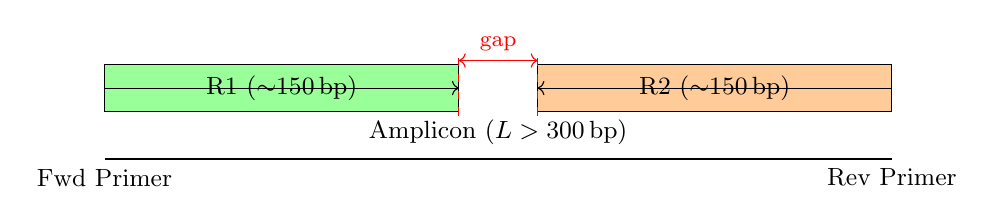
\begin{tikzpicture}[scale=1, font=\small]
  % Amplicon bar
  \draw[thick] (0,0) -- (10,0);
  \node[below] at (0,0)  {Fwd Primer};
  \node[below] at (10,0) {Rev Primer};
  \node[above] at (5, 0.05) {Amplicon ($L > 300$\,bp)};

  % R1
  \fill[green!40] (0, 0.6) rectangle (4.5, 1.2);
  \draw (0, 0.6) rectangle (4.5, 1.2);
  \node at (2.25, 0.9) {R1 ($\sim$150\,bp)};
  \draw[->] (0, 0.9) -- (4.5, 0.9);

  % R2
  \fill[orange!40] (5.5, 0.6) rectangle (10, 1.2);
  \draw (5.5, 0.6) rectangle (10, 1.2);
  \node at (7.75, 0.9) {R2 ($\sim$150\,bp)};
  \draw[<-] (5.5, 0.9) -- (10, 0.9);

  % Gap
  \draw[dashed, red] (4.5, 0.55) -- (4.5, 1.3);
  \draw[dashed, red] (5.5, 0.55) -- (5.5, 1.3);
  \draw[<->, red] (4.5, 1.25) -- (5.5, 1.25)
      node[midway, above, red, font=\footnotesize] {gap};
\end{tikzpicture}
\caption{For amplicons longer than twice the read length ($>$300\,bp with 150\,bp reads),
R1 and R2 do not meet, leaving an unsequenced gap in the centre of the amplicon.}
\label{fig:read-overlap}
\end{figure}


\paragraph{2. No read-overlap means no overlap-based error correction.}
When paired reads overlap, the same genomic position is sequenced twice (once by R1, once by
R2), enabling correction of sequencing errors by comparing the two observations.
Since our amplicons are mostly longer than the read length, the reads do not overlap and this
error-correction benefit is lost. As a consequence, a single-base mismatch in the
non-overlapping region cannot be confirmed by the mate read, which \textbf{reduces our
confidence in low-frequency variant calls} and makes quality-based filtering more important
(see Section~\ref{sec:variants}).

\paragraph{3. Adapter trimming is important for the minority of short fragments.}
Because most reads stop inside the amplified region, the majority never reach the far adapter.
The $\sim$6--11\% adapter-containing reads originate from shorter amplicons or degraded
fragments where the read length exceeds the insert size; these \emph{must} be trimmed before
alignment or the adapter sequence will cause mapping failures. For the remaining
$\sim$89--94\% of reads, trimming only removes any low-quality 3' bases.

This also has an implication for \textbf{coverage uniformity} (Section~\ref{sec:coverage}): the ends of each
amplicon (where both R1 and R2 contribute) will have higher coverage than the centre
(reached by only one read direction), producing a characteristic \emph{double-peak}
coverage profile across long amplicons.

% ============================================================
\section{Software and Tools}
\label{app:software}
% ============================================================

\begin{itemize}
    \item \textbf{samtools} v1.19.2 --- BAM handling, flagstat, idxstats, depth
    \item \textbf{FastQC} v0.12.1 --- raw and trimmed read quality control
    \item \textbf{Cutadapt} v4.6 --- adaptor contamination quantification and trimming
    \item \textbf{BLAST+} --- primer localisation against hg19
    \item \textbf{bedtools} v2.31.1 --- genomic interval operations and coverage
    \item \textbf{Mutect2} (GATK 4.5) --- somatic SNV and indel calling
    \item \textbf{VarDictJava} v1.8.3 --- somatic variant calling (amplicon-optimised)
    \item \textbf{SnpEff} v5.2 --- variant functional annotation (hg19 database)
    \item \textbf{Snakemake} v7.32.4 --- workflow management
    \item \textbf{Python / R} --- data analysis and visualisation
\end{itemize}

\bibliographystyle{plain}
\bibliography{references}

\end{document}
